\documentclass[10pt,a4paper]{article}

\usepackage{amsmath}

\usepackage{inputenc}
\usepackage{fvextra}

\usepackage{algpseudocode}
\usepackage{algorithmicx}
\usepackage{amsfonts}
\usepackage{amssymb}
\usepackage{amsthm}
\usepackage[spanish]{babel}
\usepackage{bm}
\usepackage{booktabs} % To thicken table lines
\usepackage{bussproofs}
\usepackage{caption}
\usepackage{csquotes}
\usepackage{colortbl}
\usepackage{dsfont}
\usepackage{environ}
\usepackage[shortlabels]{enumitem}
\usepackage{fancyhdr}
\usepackage{forest}
\usepackage{geometry}
\usepackage{graphicx}
\usepackage[hidelinks]{hyperref}
\usepackage{ifthen}
\usepackage{multicol}
\usepackage{multirow}
\usepackage{sidecap}
\usepackage{stmaryrd}
\usepackage{tabularx}
\usepackage{titling}
\usepackage{tikz}
\usepackage{xcolor}
\usepackage{wrapfig}
\usepackage{minted}

\usetikzlibrary{arrows}
\usetikzlibrary{arrows.meta}
\usetikzlibrary{automata}
\usetikzlibrary{calc}
\usetikzlibrary{fit}
\usetikzlibrary{matrix}
\usetikzlibrary{positioning}
\usetikzlibrary{shapes.geometric}
\usetikzlibrary{shapes.multipart}

\newcommand{\red}[1]{{\color{red}#1}}
\newcommand{\green}[1]{{\color{green}#1}}
\newcommand{\blue}[1]{{\color{blue}#1}}
\newcommand{\violet}[1]{{\color{violet}#1}}
\newcommand{\orange}[1]{{\color{orange}#1}}

\newcommand{\nat}{\mathbb{N}}
\newcommand{\reales}{\mathbb{R}}

\newtheorem{theorem}{Teorema}
\newtheorem{coro}{Corolario}
\newtheorem{proposicion}{Proposición}
\newtheorem{lema}{Lema}


\usetikzlibrary{shapes.multipart}

\tikzstyle{demoBox} = [
draw=blue!20, very thick,
rectangle split, rectangle split parts=2, rounded corners, inner xsep=0.5cm,
rectangle split part fill = {blue!20, blue!5}
]

\tikzstyle{demoPart} = [
draw=blue!20, very thick,
rounded corners, inner xsep=0.5cm,
fill = blue!5
]
%\newcommand{\qed}{\begin{flushright}
%		$\blacksquare$
%\end{flushright}}

\NewEnviron{demo}[1][]{%
	\begin{center}
		\begin{tikzpicture}
			\node [demoBox](box){%
				\textbf{\scriptsize
					DEMOSTRACIÓN #1}
				\nodepart{two}
				\begin{minipage}{0.75\textwidth}
					\vspace*{0.1cm}
					\BODY
				\end{minipage}
			};
		\end{tikzpicture}
	\end{center}
}

\NewEnviron{demoPart}[1][]{%
	\begin{center}
		\begin{tikzpicture}
			\node [demoPart](box){%
				\begin{minipage}{0.75\textwidth}
					\vspace*{0.1cm}
					\BODY
				\end{minipage}
			};
		\end{tikzpicture}
	\end{center}
}


\title{Sistemas Operativos - Apuntes para final}
\author{Gianfranco Zamboni}

\usemintedstyle[cpp]{bordeland, tabsize=2}
%%%% CONFIGURACIONES %%%%

%% La coma de los reales es un punto
\decimalpoint{}

%%% Tamaño de pagina
%\geometry{
%	includeheadfoot,
%	left=2.54cm,
%	bottom=1cm,
%	top=1cm,
%	right=2.54cm
%}

%\stul{0.1cm}{0.2ex}

%% HEADER Y FOOTER
\pagestyle{fancy}

\fancyhf{}

\fancyhead[LO]{\rightmark} % \thesection\ 
\fancyhead[RO]{\small{\thetitle}}
\fancyfoot[CO]{\thepage}
\renewcommand{\headrulewidth}{0.5pt}
\renewcommand{\footrulewidth}{0.5pt}
\setlength{\headsep}{1cm}
\setlength{\headheight}{13.07225pt}

\renewcommand{\baselinestretch}{1.2}  % line spacing

%% Links en indice 
\hypersetup{
	linktoc=all,     %set to all if you want both sections and subsections linked
	linkcolor=blue,  %choose some color if you want links to stand out
}
\setcounter{tocdepth}{2}
\begin{document}

	\maketitle
	\tableofcontents

\newpage
\section{Introducción}
\subsection{La semilla del internet}  
El telégrafo fue el antecesor del teléfono, un primer acercamiento a la comunicación de
mensajes vía una codificación. Desde fines de siglo XIX hasta segunda mitad del siglo XX,
aparecen las centrales de \textbf{conmutación de circuitos} (centrales telefónicas). A estas centrales
llegaban señales (cables) correspondientes a todas las casas que participacen en el sistema de
teléfonos. Las operadoras conectaban dos circuitos en sus tableros para cerrar el circuito y
permitir la comunicación entre las dos partes involucradas. Sin embargo, este tipo de comunicación tenía una gran falla: Si una central de conmutación de circuitos
dejaba de estar disponible por algún motivo de fuerza, todas las personas pertenecientes a esa
zona se verían incomunicadas.


A fines de los 50 se empieza a desarrollar la \textbf{conmutación de paquetes} buscando resolver este tema, es decir se busca una \textbf{red más tolerante a fallas}, \textbf{más flexible} a la hora de conectar dos puntos distantes y que \textbf{escale más facilmente} ante un incremento en el acceso a la comunicación.

La nueva red propuesta es una red descentralizada con mútiples caminos entre dos puntos que divide los paquetes en fragmentos que pueden llegar a destino a través de distintos caminos.

\subsection*{El modelo OSI}
En 1983 aparece una publicación de ISO para establecer un estándar que especifique la estructura de una arquitectura de red, que uniformice la forma de construir las redes de cominucación: el modelo OSI-ISO (Open Systems Interconnection).

\begin{figure}[h]
	\centering
	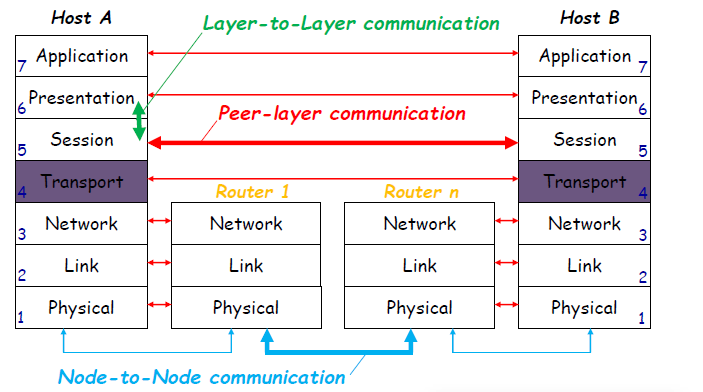
\includegraphics[width=0.65\textwidth
]{images/osi.png}
	\caption[Modelo OSI de Referencia]{Modelo OSI}
	\label{fig:osi}
\end{figure}

Este modelo está dividido en 7 capas, cada una de las cuales tiene una función definida que permitirán la comunicación coherente entre dos sistemas remotos.  

\begin{enumerate}
  \item La capa \textbf{física (Physical)} se encarga de enviar raw bits a través de los medios físicos disponibles en la red. 
  \item La capa de \textbf{enlace (Link)} se encarga de detectar errores en la transmisión y corregirlos, si es posible.
  \item La capa de \textbf{red (Network)} se encarga de resolver problemas de congestión dentro de la red, que paquetes se aceptan y la ruta que deben tomar los paquetes que se envían por la misma.
  \item La capa de \textbf{transporte (Transport)} se encarga de tomar la información provista por la capa de arriba, pasarla a la capa de red separada en pedazos más chicos (\textbf{chunks}) y se asegura que todas las partes lleguen a destino correctamente. 
  
  Esta es la primer capa \textbf{end-to-end}, es decir que entabla una ``conversación'' entre la máquina emisora (\textbf{Source}) y la destinataria (\textbf{Destination}). Las capas anteriores, usan protocolos de comunicación nodo a nodo, es decir, entre una máquina y su vecino inmediato y no entre el source y el destination que podrían estar separados entre sí por varios nodos.
  
  \item La capa de \textbf{sesión  (Session)} permite establecer sesiones entre dos máquinas distintas. Estas sesiones permiten sincronizar el pasaje de información entre ambas máquinas, deciden de quien es el turno para enviar información y evitar que ambas máquinas realizen operaciones críticas de manera simultanea.
  \item La capa de \textbf{presentación (Presentation)} procesa la información recibida, la estructura y la codifica de la manera necesaria para que pueda ser usada por la máquina.
  \item La capa de \textbf{aplicaciones (Application)} contiene los protocolos necesarios para que los usuarios puedan ver y leer la información.
\end{enumerate}

Además de estas funcionalidades, cada capa ofrece una interfaz que le permite comunicarse con las capas vecinas para hacer el pasaje de los datos entre ellas y asumen que el host en el otro extremo de la comunicación tendrá una arquitectura similar y podrá interpretar los mensajes de cada una de ellas.

\subsection{Modelo TCP/IP}
\begin{figure}[H]
	\centering
	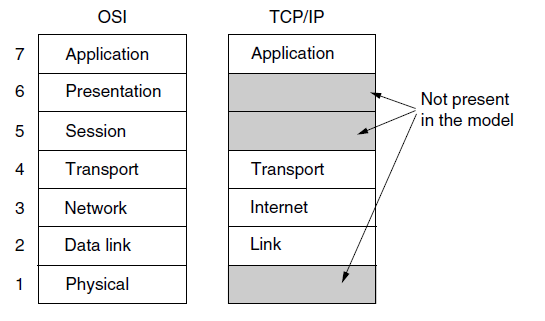
\includegraphics[width=0.65\textwidth
]{images/tcpip.png}
	\caption[Modelo TCP/IP de Referencia]{Modelo TCP/IP}
	\label{fig:tcp}
\end{figure}

Fue diseñado con el objetivo de mantener las conexiones intactas mientras ambos puntos finales de conexión estén funcionando, incluso si laguno de las máquinas o líneas entre ellos fuese dado de baja.

\begin{enumerate}
  \item La capa de \textbf{enlace (Link)} maneja la infraestructura física de la red y permite que dos nodos se puedan comunicar entre si. Se encarga de convertir los bits enviados por la capa superior a señales analógicas y transmitirlas a través de los medios físicos disponibles.
  \item La capa de \textbf{intrared (internet)} permite al host injectar paquetes en cualquier red y se encarga de hacerlos llegar a destino. Esto se hace de manera independiente para cada paquete, es decir pueden no seguir el mismo camino e incluso podrían llegar en distinto orden. En el último caso corresponde a la capas superiores reodenarlos para que puedan ser procesados, si es necesario.
  \item La capa de \textbf{transporte (Transport)} debe ser diseñada para permitir que dos entidades de la red puedan mantener una conversación. Aquí se definieron dos protocolos:
  \begin{itemize}
    \item El \textbf{Transmission Control Protocol (TCP)} que permite enviar sin errores un stream de bytes desde una máquina a otra en la red.
    \item El \textbf{User Datagram Protocol (UDP)} que permite evitar todo el flujo de conexión TCP y crear el suyo propio. En general, se usa en aplicaciones que requieren una respuesta más rápida que precisa. 
  \end{itemize}
  \item La capa de \textbf{Aplicación (Application)} es en la que se incluyen la sesiones y funciones necesarias para codificar y procesar los paquetes enviados y recibidos. Entre los protocolos usados en esta capa se encuentran: TELNET, FTP y SMTP.
\end{enumerate}


\newpage
\part{Nível Físico}
\section{Teoría de la información}
\subsection{Información}
Sea \(E\) un suceso que puede presentarse con probabilidad \(P(E)\). Cuando \(E\) tiene lugar, decimos que hemos recibido \[I(E)=\log\frac
{1}{P(E)}\] unidades de información.

Si introducimos el logaritmo de base 2, la unidad se denomina \textit{bit}. Notemos, también, que si \(P(E) = \frac{1}{2}\), \(I(E) = 1\) bit. Es decir, un bit es la cantidad de información obtenida al especificar una de dos posbiles alternativas igualmente probables.

\subsubsection{Fuentes de Memoria Nula}
Son fuentes de información que emiten una secuencia de símbolos pertenecientes a un alfabeto finito y fijo \(S=\{s_1,\dots,s_n\}\) de manera estadísticamente independientes. Estas fuentes pueden describirse mediante el alfabeto \(S\) y las probabilidades con que los simbolos se presentan: \(P(s_1), \dots, P(s_n)\).

La información que aporta cada símbolo de la fuente \[I(s_i) = \log_2\frac{1}{P(s_i)}\text{ bits}\]
\subsubsection{Entropía}
Dada una fuente de memoria nula \(S\) con alfabeto \({s_1,\dots,s_n}\), la entropía \(H(S)\) es la cantidad media de información por símbolo de la fuente, es decir:
\[H(S) = \sum_{i=1}^n P(s_i)I(s_i) = \sum_{i=1}^n P(s_i)\log_2\frac{1}{P(s_i)} = -\sum_{i=1}^n P(s_i)\log_2 P(s_i)\text{ bits} \]

Podemos interpretar la entropía como el \textbf{valor medio ponderado de la cantidad de información} del conjunto de mensajes posibles, como una medida de la \textbf{incertidumbre probmedio (grado de incerteza)}acerca de una variable aleatoria o la \textbf{cantidad de información} obtenida al observar la aparición de cada nuevo símbolo.

\paragraph{Propiedades:}
\begin{itemize}
  \item La entropía es no negativa y se anula si y solo si la probabilidad de uno de sus símbolos es 1 y la del resto es 0.
  \item La entropía máxima (\textbf{mayor incertidubme del mensaje}) se logra cuando todos los símbolos que puede ser emitidos por la fuente son equiprobables.
    \item Si hay \(n\) símbolos equiprobables \(P(s)=\frac{1}{n}\) se cumple:
    \[
      H(S) = -\sum_s P(S)\log_2 P(S) = -n(\frac{1}{n}\log_2\frac{1}{n}) = -(\log_2 1 - log_2 n) = \log_2 n
    \]
\end{itemize}

\subsubsection{Extensión de memoria nula}
Si tenemos una fuente de memoria nula \(S\), con un alfabeto \(\{s_1,\dots,s_q\}\), podemos agrupar las salidas en paquetes de \(n\) símbolos. Tendremos, pues, \(qn\) secuencias de salidas distintas. 

Formalmente, sea \(S\) una fuente de información de memoria nula con un alfabeto \(\{s_1,\dots,s_q\}\). Sea \(P_i\) la probabilidad correspondiente a \(s_i\). Entonces, la extensión de orden \(n\) de \(S\) \((S^n)\) es una fuente de memoria nula de \(qn\) símbolos \(\{\sigma_1,\dots,\sigma_{qn}\}\) donde cada \(\sigma_i\) corresponde a una secuencia de simbolos de \(S\) de longitud \(n\). La probabilidad de \(\sigma_i\), \(P_{\sigma_i}\) es la probabilidad de la secuencia correspondiente. Es decir, si \(\sigma = s_{i_1}\dots s_{i_k}\) entonces \(P(\sigma) = P_{i_1}\dots P_{i_k}\).

Puesto que un símbolo de \(S^n\) corresponde a \(n\) símbolos de \(S\), es de suponer que la entropía por símbolo de \(S^n\) sea \(n\) veces mayor que la de \(S\), osea:
\[H(S^n) = nH(S)\]

\subsection{Codificación}
Sea \(S = \{ s_1,\dots, s_q\} \) el conjunto de símbolos de un alfabeto dado. Se define un \textbf{código} como la correspondencia de todas las secuencias posibles de símbolos de \(S\) a secuencias de símbolos de algún otro alfabeto \(X =\{x_1,\dots x_r\}\). \(S\) recibe el nombre de \textbf{alfabeto fuente} y \(X\) el de \textbf{alfabeto código}.

Cuando codificamos un alfabeto fuente, buscamos lograr una representación eficiente de la información mediante la eliminación de la redundancia.q

\paragraph{Código bloque:} Es aquel que asigna cada uno de los símbolos del alfabeto fuente \(S\) a una secuencia fija de símbolos del alfabeto código \(X\). Esas secuencias fijas (secuencias de \(x_i\)) reciben el nombre de palabras
código. Denominaremos \(X_i\), a la palabra código que corresponde al símbolo \(s_i\).

\paragraph{Código no singular:} Es un código en el que todas sus palabras son distintas.

\paragraph{Extensión de orden n:} La extensión \(C^n\) de orden \(n\) de un código bloque \(C:S\to X^*\), es el código bloque que hace corresponder las secuencias de símbolos de \(S\) con las secuencias de las palabras código formadas por \(C(s_i)\). Es decir: Si \(s_i\dots s_k\in S^*\), entonces \(C^n(s_i\dots s_k) = C(s_i)\dots C(s_k)\).

\paragraph{Código univócamente decodificable:} Es aquel en el cual ninguna tira de símbolos del alfabeto código admite más de una única decodificación. Dicho de otra forma, un código bloque se dice univocamente decodificable si, y solamente si, su extensión de orden \(n\) es no singular para, cualquier valor finito de \(n\).

\paragraph{Código instantaneo:} Un código unívocamente decodificable se denomina instantáneo cuando es posible decodificar las palabras de una secuencia sin precisar el conocimiento de los símbolos que las suceden.

\paragraph{Préfijo de una palabra:} Sea \(X=x_1\dots x_m\) una palabra de un código. Se denomina prefijo de esta palabra a la secuencia de símbolos \(x_1\dots x_j\), donde \(j \leq m\).

La condición necesaria y suficiente para que un código sea instantáneo es que ninguna palabra del código coincida con el prefijo de otra.

\paragraph{Inecuación de Kraft:} Dado un alfabeto \(S = \{s_1,\dots,s_n\}\) y un alfabeto de código \(X=\{x_1,\dots,x_m\}\), es condición necesaria y suficiente, para exista un código instantáneo con palabras de longitud \(l_1,\dots,l_{n}\), que se cumpla la siguiente inecuación:
\[\sum_{i=1}^n |X|^{-l_1}\leq 1\]

\subsubsection{Codificación óptima}
Buscamos codificar un alfabeto \(S\) de tal forma que máximizar la relación entre la entropía \(H(S)\) y la longitud media del código \(L\).  Sea \(l_i\) la longitud de la palabra que codifica al símbolo \(s_i\) de la fuente, \(p_i\) la probabilidad de aparicion de \(s_i\) y \(r\) la cantidad de símbolos diferentes en el alfabeto del código entonces:

\begin{itemize}
  \item \(L = \sum p_iL_i \) es la longitud medía del código.
  \item \(\log r\) es la cantidad promedio máxima de información de un símbolo del código.
  \item \(h = \frac{H(S)}{L\log r}\) es la eficencia del código.
\end{itemize}

La máxima eficencia se logra cuando \(h = 1\). En general, esto sucede cuando se asigna las palabras de código más cortas a los símbolos de fuente más probables. También se puede deducir: \[1 \geq h \geq \frac{H(S)}{L\log r}\Rightarrow L\log r \geq H(S)\]

\paragraph{Primer teorema de Shannon (Teorema de la codificación sin ruido):} Sea \(S\) una fuente de memoria no nula, y \(S^n\) la extensión de orden \(n\) de \(S\).  Sea \(C:S^n\to X^n\) un código y \(L_n\) la longitud media de los códigos correspondientes a los símbolos de \(S^n\):
\[
    L_n = \sum_{\sigma\in S^n} C(\sigma)P(\sigma)
\]
Entones vale:
\[
    H(S) \leq \frac{L_n}{n} \leq H(S) + \frac{1}{n}
\]

Esto nos dice que el número medio de símbolos de \(C\) correspendientes a un símbolo de la fuente puede hacerse tan pequeño (pero no inferior) como la entropía de la fuente. El precio que se paga por la disminución de \(L_n\) es un aumento en la complejidad de la codificación debido al gran número de símbolos de la fuente que hay que manejar.

En particular:
\[
  H(S) = \sum_{\sigma\in S^n} C(\sigma)P(\sigma)  
\]

\paragraph{Codificador óptimo:} Es un codificador que usa la menor cantidad posible de bits para codificar un mensaje, es decir: Un codificador se dice óptimo si no existe ningún código para la misma fuente con menor longitud media.

Sea \(s_i\in S\), entonces la cantidad de bits necestarios para representarlo en un codificador óptimo es \(\lceil\frac{1}{P(s)}\rceil\) y la entropía de \[H(X) = \sum_{s\in S} P(s)\log_2\left(\frac{1}{P(s)}\right)\]

\paragraph{Codificación de Huffman:} Es una forma de definir códigos óptimos asumiendo que se conoce la probabilidad de ocurrencia de los símbolos, que la codificación es símbolo por símbolo y la probabilidad de ocurrencia de cada símbolo es independiente.

Dado un mensaje \(M\):
\begin{enumerate}
  \item Se extrae del mismo la frecuencia de cada símbolo.
  \item Se ordenan los símbolos en arbol dependiendo de la frecuencia de cada uno. Mientras más cerca de la raíz, más frecuente es el símbolo.
  \item El código de un símbolo será entonces el camino de la raíz al nodo donde está ubicado (utilizando
  ceros cuando se toma la rama izquierda y 1 cuando se toma la rama derecha).
\end{enumerate} 

Así, los símbolos más frecuentes tendrán los códigos más cortos.





\newpage
\section{Señales}
\subsection{Fundamentos de las señales}
Las señales que se envían por el canal físico para comunicar dos extremos de un canal son \textbf{ondas electromagnéticas} que se propagan a través del canal a una cierta velocidad determinada por el tipo de canal que estemos usando.


Podemos definir todas las señales con una función períodica \(f(t)\) llamada \textbf{frecuencia}. Esto significa que \(f(t) = f(t + T)\) para alguna constante \(T\). Al minimo valor positivo mayo que cero de \(T\) que cumple esto, lo llamamos \textbf{período fundamental}. \(f\) se mide en Hertz o ciclos por segundo y \(T\) en segundos. 

En base a a la frecuncia y el período de una onda definimos:

\begin{itemize}
  \item \textbf{Amplitud:} Indica la cantidad de cambios en la presión del aire. Se mide en decibeles (db o volts). Por decirlo de otra forma, la amplitud es la distancia entre el eje horizontal y el punto más alto del pico de la onda, o el punto más bajo de la depresión de la onda.
  \item \textbf{Frecuencia angular:} \(\omega = 2\pi f\) radianes por segundos.
  \item \textbf{Fase:} \(\phi\): Compara el tiempo entre dos ondas y se mide en grados, de 0 a 360. Cuando dos ondas comienzan al mismo tiempo, se dice que están en fase o alineadas en fase. Cuando una onda se encuentra ligeramente retrasada en comparación con otra onda, se dice que las ondas están desfasadas.
  \item \textbf{Longitud de onda:} Es la distancia entre los ciclos repetitivos de una onda a una frecuencia dada. Cuanto más elevada sea la frecuencia, más corta será la longitud de onda: \[\lambda = \frac{c}{f}\]
  donde \(c=3*10^8\frac{m}{s}\) es la velocidad de la luz.
\end{itemize}
\begin{figure}[H]
	\centering
	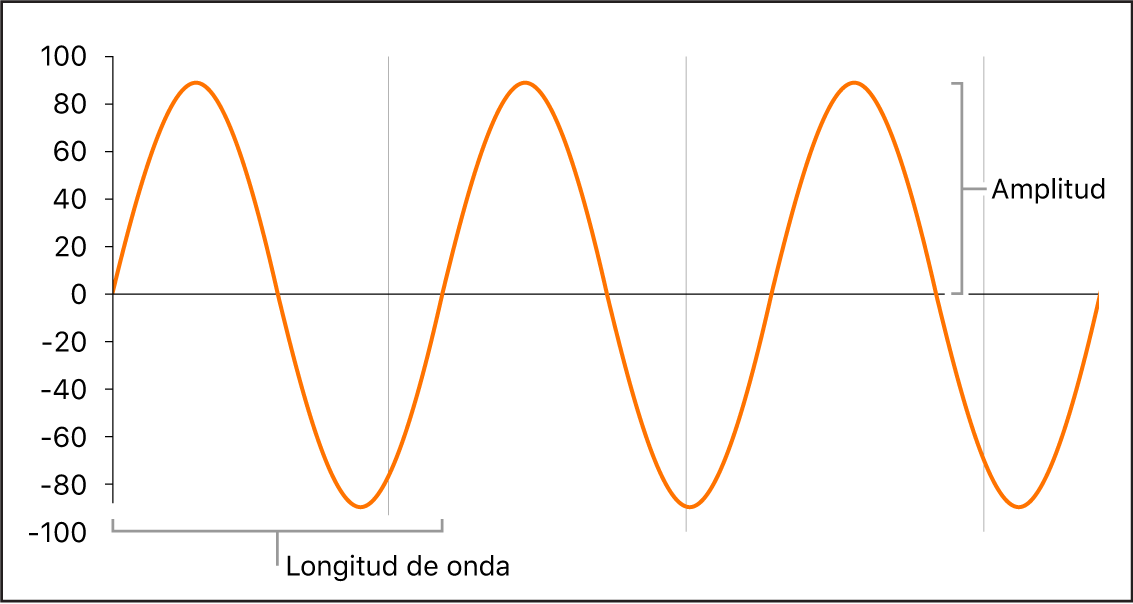
\includegraphics[width=0.65\textwidth
]{images/amplitud.png}
	\caption[Onda de señal]{Onda de señal}
	\label{fig:sistema-comunicacion-real}
\end{figure}

Esta onda puede chocar con imperfecciones del material (del canal), producir reflexiones y refracciones que se traducen en \textbf{perdidas} (menos energía para la señal original en la que está codificado el mensaje)

Dado que las ondas electromagnéticas son continuas y que son modificadas a medida que se propagan por el canal, debemos encontrar una manera de mapear estas frecuencias a los 0 y 1 que componen nuestros mensajes.

Para esto, tanto el transmisor como el recibidor definen un \textbf{ancho de banda} que es el rango de frecuencias que va a ocupar las señales que van a ser transmitidas por el canal y dentro de ese rango, cuales deben ser mapeadas a un 1 y cuales a un 0.

\subsection{Transformación de fourier}
Todas las funciones períodicas pueden expresarse como una suma infinita de senos y cosenos:

\[f(t) = \frac{1}{2}c + \sum_{i=0}^\infty \left(a_i\sen(n\omega t) + b_i\cos(n\omega t)\right)\]

done \(\omega\) es la frecuencia angular y \(a_i\) es la amplitdud de la onda.

Ninguna instalación transmisora puede transmitir señales sin perder cierta potencia en el proceso. Si todos los componentes de Fourier disminuyeran en la misma proporción, la señal resultante se reduciría en amplitud, pero no se distorsionaría. Desgraciadamente, todas las instalaciones de transmisión disminuyen los distintos componentes de Fourier en diferente grado, lo que provoca distorsión. Por lo general, las amplitudes se transmiten sin ninguna disminución desde 0 hasta cierta frecuencia \(f_c\) y todas las frecuencias que se encuentren por arriba de esta frecuencia de corte serán atenuadas. El rango de frecuencias que se transmiten sin atenuarse con fuerza se conoce como \textbf{ancho de banda}. En la práctica, el corte en realidad no es abrupto, por lo que con frecuencia el ancho de banda ofrecido va desde 0 hasta la frecuencia en la que el valor de la amplitud es atenuado a la mitad de su valor original.

El ancho de banda es una propiedad física del medio de transmisión y por lo general depende
de la construcción, grosor y longitud de dicho medio. En algunos casos, se introduce un filtro en el
circuito para limitar la cantidad de ancho de banda disponible para cada cliente.

\subsection{Problemas de los medios de transmición reales}
Cuando enviamos un mensaje a una máquina en una red, debemos pasar ese mensajes por un \textbf{transmisor} que convertirá el mensaje en una serie de \textbf{señales} que pueden ser enviadas a través del \textbf{canal} que nos comunica con la máquina de \textbf{destino}. La máquina de destino debe tener un \textbf{recibidor} que le permita captar las señales del canal y transformarlas nuevamente en el mensaje original.

Sin embargo, los canales de transmisión físicos no son perfectos y aportan \textbf{ruido} a las señales emitidas por nuestro transmisor pudiendo llegar a destino con errores.

\begin{figure}[H]
	\centering
	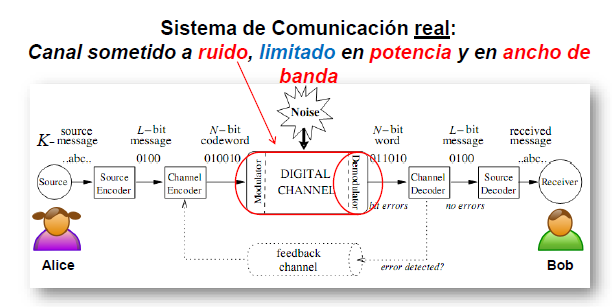
\includegraphics[width=0.65\textwidth
]{images/sistema-comunicacion-real.png}
	\caption[Esquema general de un sistema de comunicación]{Esquema general de un sistema de comunicación}
	\label{fig:sistema-comunicacion-correccion}
\end{figure}

Una forma de tratar de resolver esto es agregar al modelo nuevas capas de actores que trabajan para reducir los efectos nocivos del ruido. Por ejemplo, podemos agregar al modelo observadores externos que sean capaces de ver lo que se transmite de un lado y se recibe del otro, deducir información a partir de las diferencias, y tener chance de enviarle
correcciones al Elemento Corrector. También es posible tener dos niveles de observadores:
uno que se maneja a nivel mensaje y otro que se maneja a nivel característica del canal
propio.

\subsubsection{Tipos de errores de los canales físicos}
\begin{itemize}
  \item \textbf{Atenuación:}  En medios análogicos, la señales se degradan con la distancia recorrida lo que puede llevar a provocar errores en algunos bits recibidos. Por lo que la intensidad de la señal recibida deber ser suficiente para ser detectada y, además, debe ser suficientemente mayor al ruido del canal para que se reciba sin error. En general, las frecuencias más afectadas son las más altas por lo que se puede ecualizar estas frecuencias, es decir, amplificarlas.
  \item \textbf{Distorsión de retardo:} En medios guiados, la velocidad de propagación en el medio varía con la frecuencia por lo que los componentes del mensaje llegan en distintos instantes de tiempo, originando desplazamiento de fases entre las distintas frecuencias. Esto se puede deber a varios motivos.
\item \textbf{Ruido:} Los canales físicos poseen ruido natural. Es decir, transmiten señales adicionales debido a agentes externos:
\begin{itemize}
  \item \textbf{Ruido Término ó Ruido Blanco:} Se produce debido a la agitación térmica de electrones y aumenta linealmente con la temperatura absoluta del canal. En general, está distribuido de manera uniforme a lo largo de todo el canal y para un ancho de banda \(B\), la potencia del ruido blanco \(N_b = kTB\). 
  \item\textbf{Ruido por intermodulación:} Son señales que son la suma o la diferencia de sus frecuencias originales producidas por una falta de linealidad en el canal. \(N_I = m f_1 \pm n f_2\)
  \item\textbf{Ruido por Diafonía:} Se produce cuando una señal de una línea interfiere en otra.
  \item\textbf{Ruido impulsivo:} Son impulsos irregulares o picos que se pueden producir por interferencias externas (como pueden ser interferencia electromagnéticas, tormentas, etc). Este tipo de ruido es de corta duración, tienen gran amplitud y es disruptivo.
\end{itemize}
\end{itemize}

\subsubsection{Capacidad de un canal}
Las perturbaciones mencionadas afectan la velocidad de transmición del canal por lo que debemos asegurarnos de no enviar más bits que la capacidad límite del mismo para no perder información durante la transmición. Para esto vamos a definir los siguientes conceptos:

\begin{itemize}
  \item \(C\) es la capacidad del canal o tasa de datos, es decir a la cantidad de bits por segundo que podemos transmitir a través del mismo.
  \item \(B\) es el ancho de banda por el cual vamos a transmitir nuestros datos, va estar medido en ciclos por segundo (Hertz) y va estar limitado por el transmiso y el medio.
  \item \(N\) es el nivel medio o potencia del ruido del canal
  \item \(BER\) es la tasa de errores de bits por segundo (Bit Error Rate).
  \item \(S\) es la potencia o amplitud de la señal.
  \item \(SNR = S / N\) es la cantidad de ruido térmico presente se mide por la relación entre la potencia de la señal y la potencia del ruido, llamada relación señal a ruido. Por lo general, la relación misma no se expresa; en su lugar, se da la cantidad \(10 \log_{10} S/N\).
  Estas unidades se conocen como decibeles (dB).
\end{itemize}

En un canal sin ruido, \(C = 2B\log_2 M\) donde \(M\) es la cantidad de niveles que usamos para representar los símbolos.

En un canal con ruido, Shannon propuso
\[C_{max} = B\log_2(1 + SNR)\]

En principio, si se aumentan el ancho de banda \(B\) y la potencia de señal \(S\), aumenta la velocidad binaria. Sin embargo, un aumento de \(B\) aumenta el ruido y un aumento de \(S\) aumenta las no linealidades y el ruido de intermodulación.

\begin{figure}[H]
	\centering
	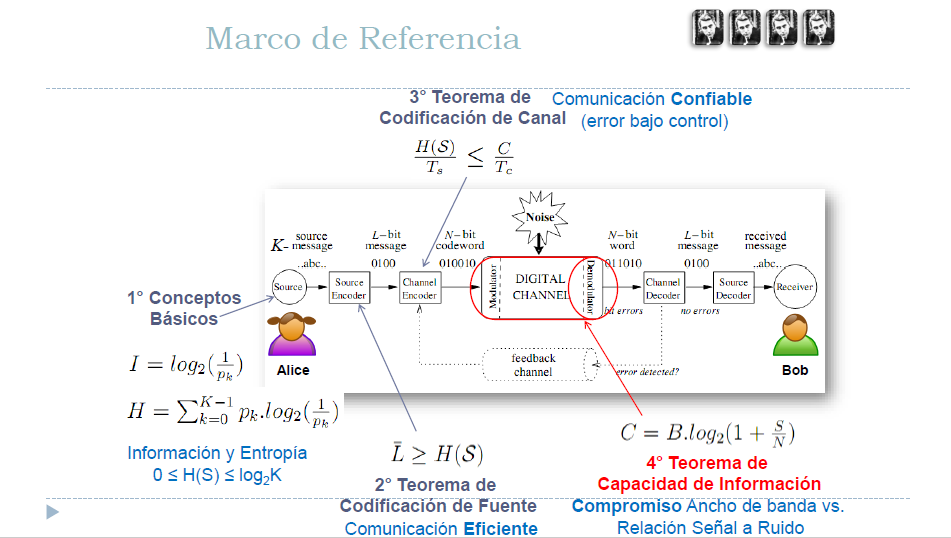
\includegraphics[width=\textwidth
]{images/marco-referencia.png}
	\caption[Esquema de un sistema de comunicación y sus conceptos asociados]{Esquema de un sistema de comunicación y sus conceptos asociados}
	\label{fig:marco-referencai}
\end{figure}


\paragraph{Límite de eficencia:} La eficiencia de ancho de banda es la máxima cantidad de bits por segundo que podemos inyectar por cada Hz sin perder información. Mientra más eficiente sea el canal, se pueden transmitir más bits por segundo. 

\paragraph{Límie de confiabilidad:} \red{Es la cantidad máxima de bits por segundos que podemos utilizar para transportar una señal de manera confiable a través de un canal ruidoso}

\subsubsection{Delay}
Por último, debemos analizar el tiempo que tarda en llegar un paquete completo desde una punta a otra de la conexión. Este tiempo se ve afectado por varias cosas:
  \begin{itemize}
    \item \textbf{Retardo de procesamiento:} Tiempo requerido en analizar el encabezado y decidir a dónde enviar el paquete. En un enrutador, dependerá del número de entradas en la tabla de rutas, la implementación (estructuras de datos), el hardware, etc. Puede incluir la verificación de errores.
    \item \textbf{Retardo de encolamiento:} Tiempo en que el paquete espera en un buffer hasta ser transmitido. El número de paquetes esperando en cola dependerá de la intensidad y la naturaleza del tráfico. Los algoritmos de colas en los enrutadores intentan adaptar estos retardos a ciertas preferencias, o imponer un uso equitativo.
    \item \textbf{Retardo de transmición:} El tiempo requerido para “empujar” todos los bits de un paquete a través del medio de transmisión. Si \(R\) es la capidad del canal, \(L\) la longitud del paquete y \(D_T\) el delay o retardo de transmición:
    \[D_T = \frac{L}{R}\]
    \item \textbf{Retardo de propagación:} Una vez que el bit es 'empujado' en el medio, el tiempo transcurrido en su propagación hasta
    el final del trayecto físico. La velocidad de propagación del enlace depende más que nada de la distancia medio físico. Si \(d\) es la distancia a recorrer y \(s\) la velocidad de propagación:
    \[D_p = \frac{d}{s}\]
  \end{itemize}

 \subsection{Medios de transmición}
 \subsubsection{Medios guiados}
 \subsubsection*{Par trenzado de cobre} Uno de los medios de transmisión más viejos, y todavía el más común. Éste consiste en dos alambres de cobre aislados, por lo regular de 1 mm de grueso. Los alambres se trenzan en forma helicoidal, igual que una molécula de DNA. Esto se hace porque dos alambres paralelos constituyen una antena simple. Cuando se trenzan los alambres, las ondas de diferentes vueltas se cancelan, por lo que la radiación del cable es menos efectiva.

La aplicación más común del cable de par trenzado es en el sistema telefónico. Casi todos los teléfonos están conectados a la compañía telefónica mediante un cable de par trenzado. La distancia que se puede recorrer con estos cables es de varios kilómetros sin necesidad de amplificar las señales, pero para distancias mayores se requieren repetidores.
    
Se pueden utilizar para transmisión tanto analógica como digital. 

El ancho de banda depende del grosor del cable y de la distancia que recorre; en muchos casos pueden obtenerse transmisiones de varios megabits/seg, en distancias de pocos kilómetros.

\subsubsection*{Coaxial}
Consiste en un alambre de cobre rígido como núcleo, rodeado por un material aislante. El aislante está forrado con un conductor cilíndrico, que con frecuencia es una malla de tejido fuertemente trenzado. El conductor externo se cubre con una envoltura protectora de plástico.

La construcción y el blindaje del cable coaxial le confieren una buena combinación de ancho de banda alto y excelente inmunidad al ruido. El ancho de banda posible depende de la calidad y longitud del cable, y de la relación señal a ruido de la señal de datos. Los cables modernos tienen un ancho de banda de cerca de 1 GHz. Los cables coaxiales solían ser ampliamente usados en el sistema telefónico para las líneas de larga distancia, pero en la actualidad han sido reemplazados
por la fibra óptica en rutas de distancias considerables. Sin embargo, el cable coaxial aún se utiliza ampliamente en la televisión por cable y en las redes de área metropolitana.

\subsubsection*{Fibra óptica:}
Un sistema de transmisión óptico tiene tres componentes: la fuente de luz, el medio de trans-
misión y el detector. Convencionalmente, un pulso de luz indica un bit 1 y la ausencia de luz in-
dica un bit 0. El medio de transmisión es una fibra de vidrio ultradelgada. El detector genera un
pulso eléctrico cuando la luz incide en él. Al agregar una fuente de luz en un extremo de una fi-
bra óptica y un detector en el otro, se tiene un sistema de transmisión de datos unidireccional que
acepta una señal eléctrica, la convierte y transmite mediante pulsos de luz y, luego, reconvierte la
salida a una señal eléctrica en el extremo receptor.

Cuando un rayo de luz pasa por un medio a otro —por ejemplo, de sílice fundida al aire—, el rayo se refracta (se dobla) en la frontera de la sílice y el aire. Un rayo de luz que incide en la frontera con un ángulo \(\alpha_1\) y que emerge con un ángulo \(\beta_1\). El grado de refracción depende de las propiedades de los dos medios (en particular sus índices de refracción). Para ángulos con incidencias mayores de ciertos valores críticos, la luz se refracta nuevamente a la sílice; ninguna parte de él escapa al aire. Por lo tanto, un rayo de luz que incide en un ángulo mayor o igual que el crítico queda atrapado den-
tro de la fibra.

Puesto que cualquier rayo de luz que incida en la frontera con un ángulo mayor que el crítico se reflejará internamente, muchos rayos estarán rebotando con ángulos diferentes. Se dice que cada rayo tiene un
modo diferente, por lo que una fibra que tiene esta propiedad se denomina \textbf{fibra multimodo}. Por otro lado, si el diámetro de la fibra se reduce a unas cuantas longitudes de onda de luz, la fibra actúa como una guía de ondas y la luz se puede propagar sólo en línea recta, sin rebotar, lo cual da como resultado una \textbf{fibra monomodo}. 

Las fibras monomodo son más caras, pero se pueden utilizar en distancias más grandes. Las fibras monomodo disponibles en la actualidad pueden transmitir datos a 50 Gbps a una distancia de 100 km sin amplificación.

\subsubsection{Medios inalámbricos}
\subsubsection*{El espectro electromagnético}
\begin{figure}[H]
	\centering
	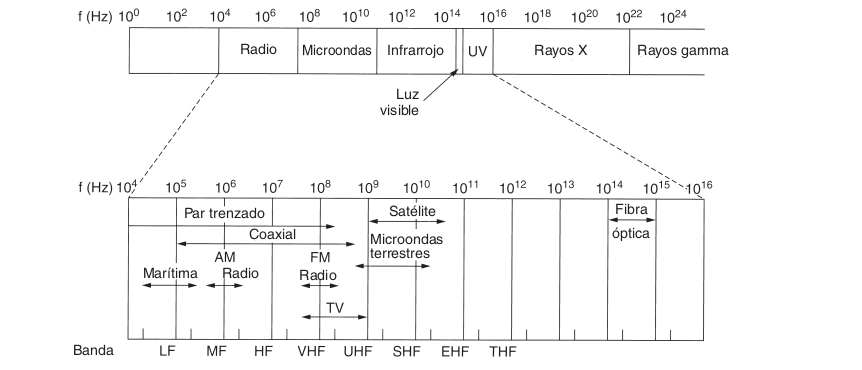
\includegraphics[width=\textwidth
]{images/espectro-magnetico.png}
	\caption[Espector magnetico]{Espector magnetico}
	\label{fig:espectro-magnetico}
\end{figure}

Las porciones de radio, microondas, infrarrojo y luz visible del espectro pueden servir para transmitir información modulando la amplitud, frecuencia o fase de las ondas. La luz ultravioleta, los rayos X y los rayos gamma serían todavía mejores, debido a sus frecuencias más altas, pero son difíciles de producir y modular, no se propagan bien entre edificios y son peligrosos para los seres vivos. 

La cantidad de información que puede transportar una onda electromagnética se relaciona con su ancho de banda. Con la tecnología actual, es posible codificar unos cuantos bits por hertz a frecuencias bajas, pero a frecuencias altas el número puede llegar hasta 8, de modo que un cable coaxial con un ancho de banda de 750 MHz puede transportar varios gigabits/seg.

A las bandas más altas se les nombró como bandas VHF (frecuencia muy alta), UHF (frecuencia ultraalta), EHF (frecuencia extremadamente alta) y THF (frecuencia tremendamente alta).

\subsubsection*{Radio}
Las ondas de radio son fáciles de generar, pueden viajar distancias largas y penetrar edificios sin problemas, y por ello su uso está muy generalizado en la comunicación, tanto en interiores como en exteriores. Las ondas de radio también son  omnidireccionales, lo que significa que viajan en todas direcciones a partir de la fuente, por lo que no es necesario que el transmisor y el receptor se encuentren alineados físicamente.

Las propiedades de las ondas de radio dependen de la frecuencia. A bajas frecuencias, esas ondas cruzan bien casi cualquier obstáculo, pero la potencia se reduce de manera drástica a medida que se aleja de la fuente.

En las bandas VLF, LF y MF las ondas de radio siguen la curvatura de la Tierra. Estas ondas se pueden detectar quizá a 1000 km en las frecuencias más bajas, y a menos en frecuencias más altas.

n las bandas HF y VHF, las ondas a nivel del suelo tienden a ser absorbidas por la tierra. Sin
embargo, las ondas que alcanzan la ionosfera, una capa de partículas cargadas que rodea a la Tie-
rra a una altura de 100 a 500 km, se refractan y se envían de regreso a nuestro planeta. En ciertas condiciones atmosféricas, las señales pueden rebotar va-
rias veces. Los operadores de radio aficionados usan estas bandas para conversar a larga distancia.
El ejército se comunica también en las bandas HF y VHF.

\subsubsection*{Láser}
La señalización óptica coherente con láseres es inherentemente unidireccional, de modo que cada edificio necesita su propio láser y su propio fotodetector. Este esquema ofrece un ancho de banda muy alto y un costo muy bajo. También es relativamente fácil de instalar.

Una desventaja es que los rayos láser no pueden penetrar la lluvia ni la niebla densa, pero nor-
malmente funcionan bien en días soleados. Sin embargo, el calor del sol causa corrientes de convección que se elevabn desde el techo de los edificio. Este aire turbulento desviaba el rayo y lo hacía danzar alrededor del detector.

\subsubsection*{Satélites}
Los satélites de comunicaciones tienen algunas propiedades interesantes que los hacen atrac-
tivos para muchas aplicaciones. En su forma más simple, un satélite de comunicaciones se puede
considerar como un enorme repetidor de microondas en el cielo. Contiene numerosos transpon-
dedores, cada uno de los cuales se encarga de una parte del espectro, amplifica la señal entrante
y a continuación la retransmite en otra frecuencia para evitar interferencia con la señal entrante.
Los haces pueden ser amplios y cubrir una fracción sustancial de la superficie de la Tierra, o es-
trechos, y abarcar sólo algunos cientos de kilómetros de diámetro. Este modo de operación se
conoce como de tubo doblado.

\subsection{Red télefonica}
La \textbf{Red Telefónica Pública Conmuta-
da} (PSTN), fue diseñadas hace muchos años, con el propósito de transmitir la voz humana en una forma más o menos reconocible.

\begin{figure}[H]
	\centering
	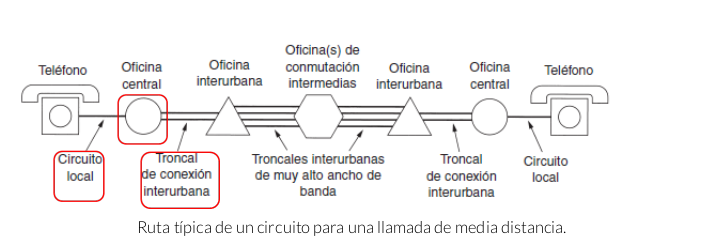
\includegraphics[width=0.9\textwidth
]{images/redes-telefonicas.png}
	\caption[Sistema  telefónico]{Sistema  telefónico}
	\label{fig:sistema-telefonico}
\end{figure}

El sistema telefónico consiste en tres componentes principales:
\begin{enumerate}
  \item Circuitos locales: Cables de par trenzado que van hacia las casas y las empresas. Dan acceso a todo mundo al sistema completo, debido a lo cual son cruciales. Por desgracia, también son la parte más débil del sistema. Cada oficina central tiene varias líneas salientes a uno o más centros de conmutación cercanos, llamados \textbf{oficinas interurbanas}.
  \item Troncales (fibra óptica digital que conecta a las oficinas de conmutación).
  \item Oficinas de conmutación (donde las llamadas pasan de una troncal a otra).
\end{enumerate}

Para las troncales de largo alcance, la principal consideración es cómo reunir múltiples llamadas y
enviarlas juntas por la misma fibra. Este tema se llama \textbf{multiplexión}.

\subsubsection{Tipos de multiplexión}
Las compañías telefónicas han desarrollado esquemas complejos para multiplexar muchas conversaciones en una sola troncal física. Estos esquemas de multiplexión se pueden dividir en dos categorías principales: FDM (Multiplexión por División de Frecuencia) y TDM (Multiplexión por División de Tiempo). En FDM el espectro de frecuencia se divide en bandas de frecuencia, y cada usuario posee exclusivamente alguna banda. En TDM los usuarios esperan su turno (en round-robin), y cada uno obtiene en forma periódica toda la banda durante un breve lapso de tiempo.

\paragraph{Multiplexión por División de Frecuencia:} Los filtros limitan el ancho de banda utilizable a cerca de 3000 Hz por canal de calidad de voz. Cuando se multiplexan muchos canales juntos, se asignan 4000 Hz a cada canal para mantenerlos bien separados. Primero se eleva la frecuencia de los canales de voz, cada uno en una cantidad diferente, después de lo cual se pueden combinar, porque en ese momento no hay dos canales que ocupen la misma porción del espectro. Hay cierta superposición entre canales adyacentes porque los filtros no tienen bordes bien definidos. Esta superposición significa que un pico fuerte en el borde de un canal se detectará en el adyacente como ruido no térmico. Para los canales de fibra óptica se utiliza una variante de la multiplexión por división de fre-
cuencia llamada \textbf{Multiplexión por División de Longitud de Onda} (WDM).

\paragraph{Multiplexión por División de Tiempo:} Aunque FDM aún se utiliza sobre cables de cobre o canales de microondas, requiere circuitos analógicos y no es fácil hacerla con una computadora. En contraste, TDM puede manejarse por completo mediante dispositivos digitales y a ello se debe su popularidad en los últimos años. Desgraciadamente, sólo se puede utilizar para datos digitales. Puesto que los circuitos locales producen señales analógicas, se necesita una conversión de analógico a digital en la oficina central, en donde todos los circuitos locales individuales se juntan para combinarse en troncales.

\subsubsection{Conversión analógico digital}
\begin{figure}[H]
	\centering
	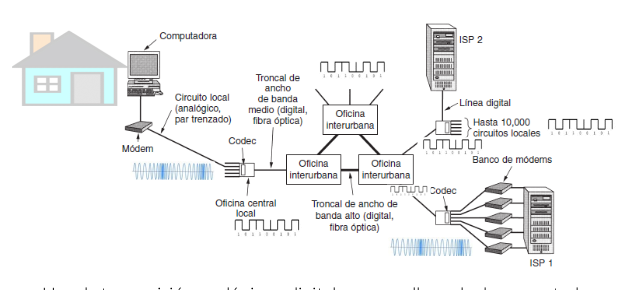
\includegraphics[width=0.9\textwidth
]{images/conversion-analogico-digital.png}
	\caption[Conversión analogico digital]{Conversión analogico digital}
	\label{fig:conversion-analogico-digital}
\end{figure}
\subsection{Modulación}
La transmición analógica se basa en una señal continua de frecuencia constante  denomidada \textbf{portadora}. La frecuencia de la portadora se elige de tal forma que sea compatible con las características del medio que se vaya a utilizar. Los datos se pueden transmitir modulando la señal portadora para asegurarnos de que llegue al próximo extremo sin perder información. Todas las técnicas de modulación implican la modificación de uno o más de los tres parámetros fundamentales de la frecuencia portadora: amplitud, frecuencia y fase.

La señal de entrada \(m(t)\) se denomina señal \textbf{moduladora} a la señal resultante de la modulación de la señal portadora.

Hay distintos tipos de modulaciones:

\begin{itemize}
  \item \textbf{Desplazamiento de amplitud (ASK):} Los dos valores binarios se represnetan mediante dos amplitudes diferences de la portadora. Es usual que una de las amplitudes sea cero.
  \[
    S(t) = \begin{cases}
      A\cos(2\pi f_c t) & \text{1 binario} \\
      0 & \text{0 binario}
    \end{cases}
  \]

  ASK es sensible a cmabios repentinos de la ganancia, además es una técnica de modulación bastante ineficaz. Se usa para la transmición de datos digitales en fibras ópticas
  \item  \textbf{Desplazamiento de frecuencia (FSK):} Los dos valores binarios se representan mediante dos frecuencias diferentes próximas a la frecuencia portadora. La señal resultante es
  \[
    S(t) = \begin{cases}
      A\cos(2\pi f_1 t) & \text{1 binario} \\
      A\cos(2\pi f_2 t) & \text{0 binario}
    \end{cases}
  \]
  
  donde \(f_1\) y \(f_2\) corresponden a desplazamientos de la frecuencia portadora \(f_c\), de igual magnitud pero en sentidos opuestos.

  FSK es menos sensible a errores que ASK.
  \item  \textbf{Desplazamiento de fase (PSK):} La fase de la señal portadora se despaza para representar con ello a los datos digitales: En este sistema, un cero binario se representa mediante la transmición de una señal con la misma fase que la fase de la señal anteriormente enviada. Mientras que un uno se representa mediante la transmición de una señal cuya fase esté en opociión de fase respecto de la señal precente. Esta técnica se conoce como PSK diferencial, ya que el desplazamiento en fase es relativo a la fase correspondiente al último símbolo transmitido.
  
  \[
    S(t) = \begin{cases}
      A\cos(2\pi f_c t + \pi) & \text{1 binario} \\
      A\cos(2\pi f_c t) & \text{0 binario}
    \end{cases}
  \]
\end{itemize}

\paragraph{Velocidad de modulación:} El número de cambios de señal por unidad de tiempo. Se expresa en \textbf{baudios} (símbolos por segundo).

\paragraph{Velocidad de transmición:} Equivale a la velocidad de modulación multiplicado por el número de bits \(N\) represenntados por cada símbolo. Se expresa en bits por segundo: \(V_t = V_m\cdot m\)

Se puede conseguir una utilización más eficaz del ancho de banda si cada elemento de señalización representa más de un bit.  En el métood PSKQ  considera desplazamientos de fase correspondientes a \(\pi/2\) (\(90°\)) por lo que cada señal representa dos bits en lugar de uno:
\[
  S(t) = \begin{cases}
    A\cos(2\pi f_c t + \frac{\pi}{4}) & \text{11} \\
    A\cos(2\pi f_c t + \frac{3\pi}{4}) & \text{10} \\
    A\cos(2\pi f_c t + \frac{5\pi}{4}) & \text{00} \\
    A\cos(2\pi f_c t + \frac{7\pi}{4}) & \text{01} \\
  \end{cases}
\]

\subsubsection{Codificación}
Una vez modulada, la señal analógica viaja hasta un \textbf{codec}  en la oficina central  que se encarga de digitalizarla. El codec toma 8000 muestras por segundo porque el teorema de Nyquist dice que esto es suficiente para capturar toda la información del ancho de banda de 4 kHz del canal telefónico. A una velocidad de muestreo menor, la información se perdería; a una mayor, no se ganaría información extra. Esta técnica se llama \textbf{Modulación por Codificación de Impulsos} (PCM).   

A veces, se usa un técnica conocida como \textbf{Modulación Delta}, en el que la entrada analógica se aproima mediante una función escalera que en cada intervalo de muestreo (\(T_S\)) sube o bajaa un nivel de cuantización \(\delta\). La característica principal de la función escalera es qeu su comportamiento es binario: En cada instante de muestreo, la función sube o baja una cantidad constante. Por tanto, la salida del modulador delta se puede representar mediante un único bit para cada muestra. Resumiendo: se obiente una cadena de bits que aproxima a la derivada de la señal analógica de entrada en cualquier lugar de la amplitud.

\subsubsection*{No retorno a cero (NRZ)}
La forma más frecuente y fácil de transmitir señales digitales es mediante la utilización de un nivel diferente de tensión para cada uno de los dos dígitos binatios. Los códigos que siguen esta estrategia comparten la propiedad de que el nivel de tensión se mantiene constante durante la duración del bit. Es habitual usar un nivel negativo para representar un valor binario y un tensión positiva para representar el otro.

Una variante de este código de nomina \textbf{No retono a Cero con Inversion de unos} (NZRI) en la que un 1 se codifica mediante la transición al principio del intervalo de señalización, mientras que un 0 se rpresenta por la ausencia de transición. Esta codificación es un ejemplo de codificación diferencial, en lugar de determinar el valor absoluto, la señal se codifica comparando la polaridad de los elementos de señal adyacentes.

\subsubsection*{Codificación Manchester (Bifase)}
El valor de un bit se códifica en una transición a la mitad del intervalo de duración del bit. Esta transición en la mitad del bit sirve como un procedimiento de sincronización a la vez que sirve para transmitir los datos: Una transción de bajo a alto representa un 1 y una transición de alto a bajo representa un cero.

En Mancheste diferencial, la transición a mitad del intervalo se utiliza tan solo para proporcionar sincronización. La codificación de un cero se representa por la presencia de una trancisión al principio del intervalo. 

Toda técnica bifase fuerzan al menos una transición por cada bit pudiendo tener hasta dos en ese mismo período. Por tanto, la velocidad de modulación máxia es el doble que en los NRZ y el ancho de banda necesario es mayor.

\subsection{Redes de conmutación}
En la actualidad se utilizan dos técnicas de conmutación diferentes: conmutación de circuitos y conmutación de paquetes. A continuación presentaremos una breve introducción a cada una de ellas.

\subsubsection*{Conmutación de circuitos}
Cuando se realiza una llamada telefónica, el equipo de conmutación del sistema telefónico busca una trayectoria física que vaya desde su teléfono al del receptor. Esta técnica se llama \textbf{conmutación de circuitos}.

Una propiedad importante de la conmutación de circuitos es la necesidad de establecer una trayectoria de un extremo a otro antes de que se pueda enviar cualquier dato. El tiempo que transcurre entre que se termina de marcar y que el timbre comienza a sonar puede ser fácilmente de 10 seg, y más en las llamadas de larga distancia o internacionales. Durante este intervalo de tiempo, el sistema telefónico busca una trayectoria de cobre. La señal de petición de llamada se debe propagar hasta el destino y se debe confirmar su recepción. En muchas aplicaciones de computadora, los tiempos de establecimiento largos son indeseables.

Por otro lado, al existir una trayectoria de cobre entre las partes en comunicación, una vez que se termina de establecer, el único retardo de los datos es el tiempo de propagación de la señal electromagnética y no
hay peligro de congestión; es decir, una vez que la llamada entra, no hay posibilidad de obtener una señal de ocupado, aunque podría obtener una antes de establecer la conexión debido a la falta de capacidad de conmutación o de troncal.

\subsubsection*{Conmutación de paquetes}
La alternativa a la conmutación de circuitos es la \textbf{conmutación de paquetes}. Con esta tecnología, los paquetes individuales se envían conforme se necesite, y no se les asigna por adelantado ninguna trayectoria dedicada.

En este caso, al no ser necesaria una conexión previa, el primer paquete se puede enviar apenas esté listo. 

Con la conmutación de paquetes no
hay trayectoria, por lo que diferentes paquetes pueden seguir trayectorias distintas, dependiendo
de las condiciones de la red en el momento en el que se enviaron. Pueden llegar en desorden.

La conmutación de paquetes es más tolerante a las fallas que la conmutación de circuitos. De  hecho, ésa es la razón por la cual se inventó. Si falla la conmutación, todos los circuitos que la están utilizando se cancelan y no se puede enviar nada más a través de ellos. Con la conmutación de pa-
quetes, los paquetes pueden enrutarse evitando a los conmutadores averiados.

La conmutación de paquetes utiliza transmisión de almacenamiento y reenvío. Un paquete se
almacena en la memoria del enrutador y luego se reenvía al siguiente enrutador. Con la conmuta-
ción de paquetes los bits simplemente fluyen de manera continua a través del cable. La técnica de
almacenamiento y reenvío agrega retardo.

\newpage
\section{Nivel de enlace}
La capa de enlace de datos tiene que desempeñar varias funciones específicas, entre las que
se incluyen:
\begin{itemize}
  \item Proporcionar una interfaz de servicio bien definida con la capa de red.
  \item Manejar los errores de transmición.
  \item Regular el flujo de datos para que receptores lentos no sean saturados por emisores rápidos.
\end{itemize}
Para cumplir con estas metas, la capa de enlace de datos toma de la capa de red los paquetes y los encapsula en \textbf{tramas} para transmitirlos. Cada trama contiene un \textbf{encabezado}, un campo de carga útil (\textbf{payload}) para almacenar el paquete y un \textbf{terminador} o final. El manejo de las tramas es la tarea primordial de la capa de enlace de datos.

\subsection{Servicios proporcionados}
La capa de enlace de datos puede diseñarse para ofrecer varios servicios. Los servicios reales
ofrecidos pueden variar de sistema a sistema. Tres posibilidades razonables que normalmente se
proporcionan son:
\begin{enumerate}
  \item \textbf{Servicio no orientado a la conexión sin confirmación de recepción:} Consiste en hacer que la máquina de origen envíe tramas independientes a la máquina de destino sin pedir que ésta confirme la recepción. No se establece conexión de antemano ni se libera después. Si se pierde una trama debido a ruido en la línea, en la capa de enlace de datos no se realiza ningún intento por detectar la pérdida ni por recuperarse de ella.
  \item \textbf{Servicio no orientado a la conexión con confirmación de recepción:} Cuando se ofrece este servicio tampoco se utilizan conexiones lógicas, pero se confirma de manera individual la recepción de cada trama enviada. De esta manera, el emisor sabe si la trama ha llegado bien o no. Si no ha llegado en un tiempo especificado, puede enviarse nuevamente.
  \item \textbf{Servicio orientado a la conexión con confirmación de recepción:} Con este servicio, las máquinas de origen y de destino establecen una conexión antes de transferir datos. Cada trama enviada a través de la conexión está numerada, y la capa de enlace de datos garantiza que cada trama enviada llegará a su destino. Es más, garantiza que cada trama será recibida exactamente una vez y que todas las tramas se recibirán en el orden adecuado.
\end{enumerate}

\subsection{Separación de frames:}
Puesto que es demasiado riesgoso depender de la temporización para marcar el inicio y el final de cada trama, se han diseñado otros métodos:

\begin{enumerate}
  \item \textbf{Largo fijo:} Todos los paquetes tienen la misma longitud.
  \item \textbf{Conteo de caracteres}: Se vale de un campo en el encabezado para especificar el número de caracteres en la trama. Cuando la capa de enlace de datos del destino ve la cuenta de caracteres, sabe cuántos caracteres siguen y, por lo tanto, dónde está el fin de la trama. El problema con este algoritmo es que la cuenta puede alterarse por un error de transmisión. Si esto pasa, el destino perderá la sincronía y será incapaz de localizar el inicio de la siguiente trama. Incluso si el destino sabe que la trama está mal porque la suma de verificación es incorrecta, no tiene
  forma de saber dónde comienza la siguiente trama. Regresar una trama a la fuente solicitando una retransmisión tampoco ayuda, ya que el destino no sabe cuántos caracteres tiene que saltar para llegar al inicio de la retransmisión.
  \item \textbf{Flags con bit-stuffing}: El segundo método de entramado evita el problema de tener que sincronizar nuevamente después de un error, haciendo que cada trama inicie y termine con bytes especiales llamado \textbf{flags}. De esta manera, si el receptor pierde la sincronía simplemente puede buscar la bandera para encontrar el final e inicio de la trama actual. Dos banderas consecutivas señalan el final de una trama y el inicio de la siguiente. 
  
  Cuando se utiliza este método para transmitir datos binarios, como programas objeto o números de punto flotante, surge un problema serio. Se puede dar el caso con mucha facilidad de que el patrón de bits de la bandera aparezca en los datos (payload), lo que interferiría en el entramado. Una forma de resolver este problema es hacer que la capa de enlace de datos del emisor inserte un byte de \textbf{escape especial} (ESC) justo antes de cada bandera “accidental” en los datos. La capa de enlace de datos del lado receptor quita el byte de escape antes de entregar los datos a la capa de red. Esta técnica se llama \textbf{relleno de caracteres} o bit-stuffing. Por lo tanto, una bandera de entramado se puede distinguir de uno en los datos por la ausencia o presencia de un byte de escape que la antecede.
\end{enumerate}

\subsection{Detección y corrección de errores}

Los diseñadores de redes han desarrollado dos estrategias principales para manejar los errores. Una es incluir suficiente \textbf{información redundante} en cada bloque de datos transmitido para que el receptor pueda deducir lo que debió ser el carácter transmitido. La otra estrategia es incluir sólo suficiente redundancia para permitir que el receptor sepa que ha ocurrido un error (pero no qué error) y entonces solicite una retransmisión. La primera estrategia utiliza \textbf{códigos de corrección de errores}; la segunda usa \textbf{códigos de detección de errores}. 

\subsubsection{Detección de errores}
\paragraph{Bit de paridad:} La forma más sencilla. Consiste en añadir un bit de paridad al final del bloque de datos. El valor de ese bit se determina de tal forma que el código resultante tenga un número impar de unos. El receptor examina el código recibido y, si el número total es impar, supondrá que no ha habido errores. 

La utilización de bits de paridad no es infalibre, ya que los impulsos de ruido son a veces lo suficientemente largos como para destruir más de un bit.

\paragraph{Comprobación de redundancia cíclica (CRC):} Dado un bloque o mensaje de \(k\)-bits, el trasmisor genera una secuencia de \(n\)-bits denominada \textbf{secuencia de comprobación de la trama} de tal manera que la trama resultante con \(n+k\) bits, se divisible por algún número determinado. El receptor entonces divirá la trama recibida por ese número y, si no hay resto en la división, se supone que no ha habido errores.

\subsubsection{Códigos de corrección de errores}
Por lo general, una trama consiste en \(m\) bits de datos (es decir, de mensaje) y \(r\) bits redundantes o de verificación. Sea la longitud total \(n\) (es decir, \(n = m + r\)). A una unidad de \(n\) bits que contiene datos y bits de verificación se le conoce como palabra codificada de \(n\) bits.

Dadas dos palabras codificadas cualesquiera es posible determinar cuántos bits correspondientes difieren aplicando un OR exclusivo a las dos palabras codificadas y contar la cantidad de bits 1 en el resultado. La cantidad de posiciones de bits en la que difieren dos palabras codificadas se llama \textbf{distancia de Hamming}. Si dos palabras codificadas están separadas una distancia de Hamming \(d\), se requerirán \(d\) errores de un bit para convertir una en la otra.  

Para detectar \(e\) errores se necesita un código con distancia \(e + 1\), pues con tal código no hay manera de que \(e\) errores de un bit puedan cambiar una palabra codificada válida a otra. Cuando el receptor ve una palabra codificada no válida, sabe que ha ocurrido un error de transmisión. De manera similar, para corregir \(e\) errores se necesita un código de distancia \(2e + 1\), pues así las palabras codificadas legales están tan separadas que, aun con \(e\) cambios, la palabra codificada original sigue estando más cercana que cualquier otra palabra codificada, por lo que puede determinarse de manera única. 

\subsection{Protocolos de Transmición confiable}
\subsubsection{Stop \& Wait}
\begin{figure}[H]
	\centering
	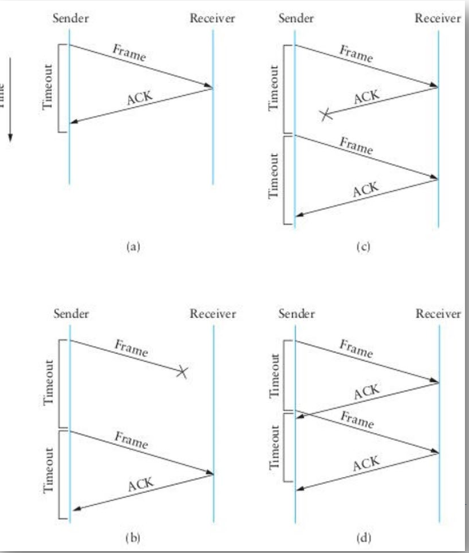
\includegraphics[width=0.65\textwidth
]{images/stop-wait.png}
	\caption[Protocolo Stop And Wait]{Protocolo Stop And Wait}
	\label{fig:stop-wait}
\end{figure}
La máquina de origen emite un único frame y espera la recepción de una confirmación (ACKnowledgment) durante un período determinado de tiempo \(t\). Mientras tanto no podrá enviar ningún otro frame.


Pueden surgir dos problemas durante la comunicación:
  
El receptor detecta algún error, entonces descartará el frame y no manda el ACK. El temporizador expira antes de la recepción del ACK y re-envía el último frame.

Por otro lado, si el frame llega correctamente y el receptor envía una ACK pero el ACK se pierde en el camino, tambien expira el temporizado y el origen vuelve a enviar el mismo frame. 
  
El destino recibe por segunda vez el frame como si fuese un frame distinto.

Para evitar este problema, los frames se etiquentan alternadamente con 0  1, y las confirmaciones positivas serán de la forma ACK0 y ACK1. Un ACK0 confirma la recepción de un frame numerada con 0 e indica que el receptor está esperando para aceptar un frame numerado con 0.

Ahora, cuando el receptor reciba dos frames con la misma numeración, podrá interpretar que está recibiendo un frame duplicado porque su ACK se perdió en el camino. En este caso, el receptor descartará el frame y volverá a mandar el ACK correspondiente.

\paragraph{Eficiencia de un protocolo:} 
Vamos a definir:
\begin{itemize}
  \item \(T_{tx}\) el tiempo de transmición de un frame (lo que tarda en ir desde el origen hasta el destino).
  \item \(RTT(F)\) el tiempo de retorno del ACK, osea el tiempo que tarda en llegar el frame al receptar sumado al tiempo que tarda en llegar el ACK al emisor original. En genaral va a pasar que \(RTT(F) = Delay\times 2\) 
\end{itemize}

El rendimiento de un protocolo \(\eta\) se define como:

\[\eta_{proto} = \frac{T_{tx}(F)}{RTT(F)}\]

\subsection{Ventana deslizante}
Aumentar la eficiencia \(eta\), implica disminuir al minimo la cantidad de tiempo que el origen se bloquea durante la espera de un ACK.

Una estrategia posible para esto es enviar varios frames seguidos, sin esperar ACKs para cada uno.
Aparece el concepto de \textbf{ventana de frames}: en una ventana se envía una cierta cantidad de frames. Esto resulta en una definición diferente para la eficiencia:

\[\eta_{proto} = \frac{T_{tx}(V)}{RTT(F)}\]

donde \(T_{tx}(V)\) es el tiempo de transmición de una ventana.

Sea \(V_{tx}\) la velocidad de transmición, definimos la capacidad de volumen de un canal \(C_{vol} = V_{tx}\times Delay\) como la cantidad de bits que entran en un canal de manera simultáneas sin saturarlo. Con esto, podemos calcular el \textbf{Sliding Window Size (SWS)} de la siguiente manera:

\[SWS = \frac{V_{tx}\times RTT(F)}{|Frames|} \text{ frames}\]

Al comenzar la comunicación, la máquina origen manda \(SWS\) frames al máquina destino. Y espera a recibir el ACK del primer frame enviado. Cuando esto sucede, el origen manda el siguiente frame de la secuencia.

Por cada ACK recibido, el origen va mandando de a uno los frames restantes siempre y cuando el último frame enviado pertezca a una ventana que contenga al frame del último ACK recibido.

\begin{itemize}
  \item \textbf{ACKs Acumulativos:} Si un ACK se pierde, el receptor descarta todos los paquetes hasta que reciba el paquete que está esperando. Esto va a provocar que se produzca un timeout en el emisor del primer paquete perdido y de todos los siguientes, por lo que volverá a enviar todos los frames de nuevo desde el último ACK recibido.
  \item \textbf{ACKs Selectivos:} El receptor recibe y se guarda todos los frames que van llegando. Supongamos que recibe el frame \(i\) con errores. Cuando llega el frame \(i + 1\) responde al receptor con un NAK\(i\). Esto le indica al emisor que si bien recibió el último paquete enviado, hubo un error en el frame anterior y tiene que reenviarlo.
  
  El receptor sigue aceptando frames y respondiendo con ACK\(i-1\) hasta que consigue correctamente el frame perdido. En este momento, responde con un ACK\(j\) donde \(j\) corresponde con el último frame que recibió sin error.
\end{itemize}

Los frames están enumerados de manera cíclica desde 1 hasta \(SWS + RWC\) donde \(RWC\) es el tamaño de la ventana de recepción y se define de la siguiente manera:

\[
  RWC = \begin{cases}
    SWS & \text{si hay ACKs Selectivos} \\
    1 & \text{si hay ACKs Acumulativos}
  \end{cases}
\]

\begin{figure}[H]
	\centering
	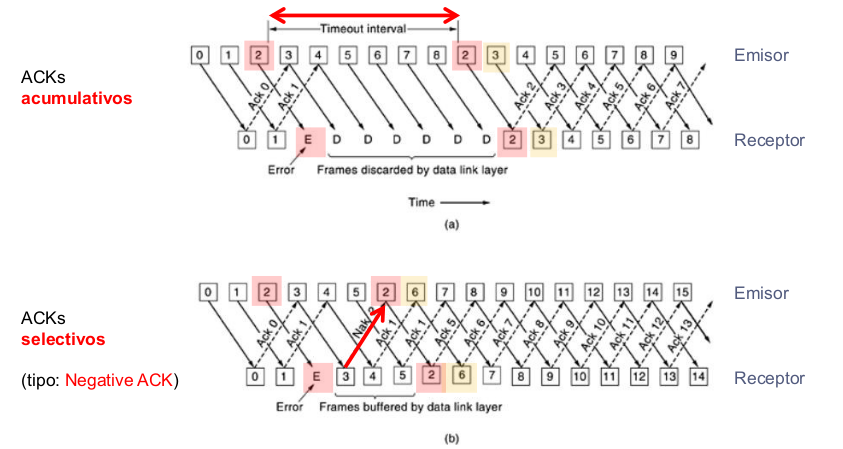
\includegraphics[width=\textwidth
]{images/sliding-window.png}
	\caption[Protocolo Sliding Window]{Protocolo Sliding Window}
	\label{fig:sliding-window}
\end{figure}

\newpage
\section{Medios Compartidos}
La idea es controlar el acceso a los medios compartidos de manera tal que haya la menor cantidad de intervención humana posible en el proceso. Es decir, se busca no tener la figura de un administrador que tenga que solucionar manualmente las cosas.

Tanto TDM, FDM, WDM y CDMA (Code Division Multiple Access) comparten una característica: debe estar decidido a priori qué usuario está usando qué parte del tiempo, frecuencia, etc. en cada momento. Para eso es necesario saber de antemano cuántos usuarios tendrá el sistema. Esto requiere un administrador dedicado a una red con características estáticas, rígidas.

Esto no escala de manera automática, por lo que no cumple la idea mencionada arriba. Esto no significa que estas técnicas no se usen: se utilizan frecuentemente en las redes
troncales (backbones), que no tienen una cantidad constantemente cambiante de nodos como sí puede tener algo como una red LAN, o Wi-Fi. Una alternativa a esto, para redes donde la cantidad de nodos es desconocida y cambiante, es la \textbf{contención estadística}. Esto se refiere a sistemas en los cuales varios usuarios comparten un canal común, de modo tal que puede dar lugar a conflictos conocidos como sistemas de
contención. Estos conflictos son aceptados y/o manejados.

\paragraph{Problemas de acceso:} Si hay varios nodos que usan un medio físico compartido, la simultaneidad de transmisión no es posible (no pueden transmitir todos a la vez). Para esto aparecen los \textbf{MAC Protocols (Medium Access Control)}, protocolos que buscan maximizar, en promedio, el número de éxitos en los intentos de comunicación, y asegurar la igualdad de oportunidades (en promedio) entre todos los nodos competidores.

En estos casos, el control es descentralizado, y surge la necesidad de un esquema de direccionamiento y de controlar el acceso.

Ejemplos: Aloha, Ethernet, Wi-Fi, Token Ring.

\subsection{Ethernet (IIEEE 802.3)}
Las computadoras de un edificio se conectan entre sí por medio de cables. Cada versión de Ethernet tiene un máximo de distancia física entre segmentos. Para permitir conexiones de mayor distancia se pueden utilizar \textbf{repetidores}, que son dispositivos que amplifican y retransmiten señales en ambas direcciones.
El formato utilizado para enviar mensajes en la red es el siguiente:

\begin{figure}[H]
	\centering
	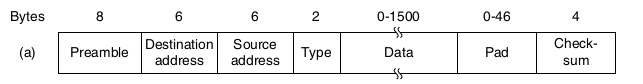
\includegraphics[width=\textwidth
]{images/ethernet-mac-frame.png}
	\caption[Frame del protocolo Ethernet]{Frame del protocolo Ethernet}
	\label{fig:ethernet-mac-frame}
\end{figure}

\begin{itemize}
  \item Los primeros 8 bytes son un preambulo que permiten a los receptors sincronizarse con la señal.
  \item Luego, vienen dos direcciones, cada uno de 6 bytes. 
  
  Cuando el primer bit de la dirección de destino es un 0, significa que el paquete está dirigido a una máquina específica.  Si es un 1, entonces es un dirección grupal: Estas direcciones permiten que varias máquinas escuchen una única dirección y que todas las máquinas pertenecientes al grupo reciban los paquetes dirigidas a esa dirección. Este tipo de envío se llama \textbf{multicasting}. Además, la dirección especial que consiste en todos bits de valor 1 está reservada para hacer \textbf{Broadcasting} (enviar un mensaje a todos los dispositivos de la red).
  \item Los próximos 2 bytes identifican el tipo de protocolo que debe usarse para procesar el contenido del paquete.
  \item Después viene la información per se que puede ocupar hasta 1500 bytes (un valor decidido de manera arbitraria).
  \item Si la data enviada es menor a 46 bytes, se usa padding hasta completar los 46 bytes necesarios para cumplir con los requirimientos de longitud mínima del mensaje. Esta longitud mínima permite que la máquina de origen detecte colisiones durante la transmición, en el caso de haberlas (más adelante explicado).
  \item Los últimos 4 bytes del paquete son un checksum (CRC de 32 bits) que permite detectar si hubo algún error en el frame, si lo hubo, el frame se descarta.
\end{itemize}

\subsubsection{Colisiones}
Una de las razones para tener una longitud mínima de un frame es para evitar que una máquina termine de transmitir el frame antes de que el primer bit haya alcanzado el otro extremo del cable, donde podría colisionar con otro frame.

\begin{figure}[H]
	\centering
	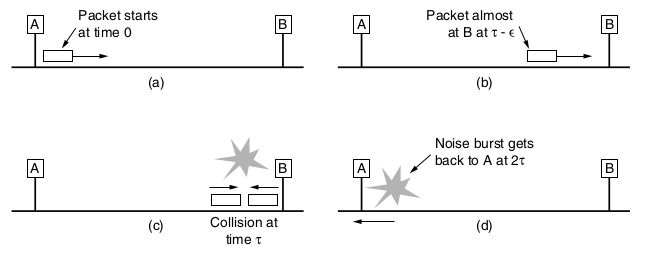
\includegraphics[width=\textwidth
]{images/deteccion-colisiones.png}
	\caption[Detección de Colisiones]{Detección de Colisiones}
	\label{fig:deteccion-colisiones}
\end{figure}

Supongamos que en un timpo 0, el host \(A\) comienza a transmitir el paquete. Sea   \(\tau\) el tiempo de propagación necesario para que el frame llegue al host \(B\). Supongamos que justo antes de que el frame llegue a destino, en el tiempo \(\tau-\epsilon\), \(B\) comienza a transmitir. Cuando \(B\) detecta que está recibiendo más energía que la que está emitiendo, se da cuenta que ocurre una colisión, aborta su propia transmisión y genera una rafaga de sonido ee 48 bits para alertar a las demás estaciones. 

En otras palabras, genera interferencia para asegurarse que el emisor (\(A\)) se de cuenta de que ocurrió la colisión. En el momento \(2\tau\), \(A\) ve el sonido y aborta su propia transmición. Luego espera un intervalo de tiempo random antes de intentar de nuevo.

Si \(A\) trata de enviar un frame muy corto, puede llegar a pasar que termine de trasmitir antes de que  perciba el ruido generado por \(B\) (en el momento \(2\tau\)). Entonces \(A\) concluiria que el frame se envió correctamente. Por esta razón, se utiliza el pading en el frame de Ethernet para completar la longitud mínima de 64 bytes.

Este valor se deduce de las especificacioens de IIEEE 802.3: Para una red de 10Mbps con una longitud de 2500 metros y a lo sumo 4 repetidores, se determinó que el round-trip time es de 50 \(\mu\)segundos, asi que 500 bits es el frame más corto posible para detectar colisiones. Este valor se redondeó a 512 bits (64 bytes).

\subsubsection{CSMA/CD con Exponential BackOff}\label{section::csma}
CSMA/CD (Carrier Sense Multiple Access with Collision Detection), es decir, acceso múltiple con sensado de portadora y detección de colisiones, es un algoritmo de control de acceso a un medio compartido.

Utiliza el sensado de portadora para determinar si hay nodos transmitiendo. Cuando un host tiene datos para enviar, sensa el medio compartido:
\begin{itemize}
  \item Si el medio está libre, el host transmite.
  \item Si el medio está ocupado, no puede enviar porque habría una colisión. Entonces debe esperar a que el medio se libere:
  \begin{itemize}
    \item Si el algoritmo es \textbf{1-persistente}, el host comienza a transmitir apenas se libere el medio.
    \item Si es \textbf{p-persistente}, el host espera a que se libere el medio y transmite con probabilidad \(p\). El uso de un componente azaroso (en la p-persistencia) tiene sentido porque si hay varios
    hosts esperando a que se libere el medio, y todos intentan transmitir ni bien éste se libera, va
    a ocurrir una colisión. Imponer una probabilidad para transmitir reduce las probabilidades de
    colisiones.
  \end{itemize}
\end{itemize}

Este algoritmo es de categoría half-duplex: La lógica de recepción está establecida en el sensado para detectar colisiones. Es decir, no se puede enviar y recibir a la vez (eso sería full-duplex).

Supongamos ahora que ocurre una colisión, entonces el tiempo se divide en slots de tamaño \(2\tau\). Después de la primera colisión, cada estación espera 0 o 1 slots de tiempo al azar. Si dos estaciones colisionan y eligen el mismo número, cada una elige entre 0, 1, 2 ó 3 tiempos al azar y espera el número de slots de tiempos elegidos antes de volver a intentar transmitir.

En general, después de la \(i\)-ésima colisión, cada host debe elegir un número entre 0 y \(2^i-1\) que será la cantidad de slots de tiempo que debe dejar pasar antes de volver a intentar la transmición.

Este algoritmo se llama \textbf{Exponential Backoff Binario}, sirve para adaptar de manera dinámica el número de estaciones que están tratando de emitir simultaneamente. Si el intervalo de elección para todas las elecciones fuese 1023, las chances de colisión son despreciables.


\begin{figure}[H]
	\centering
	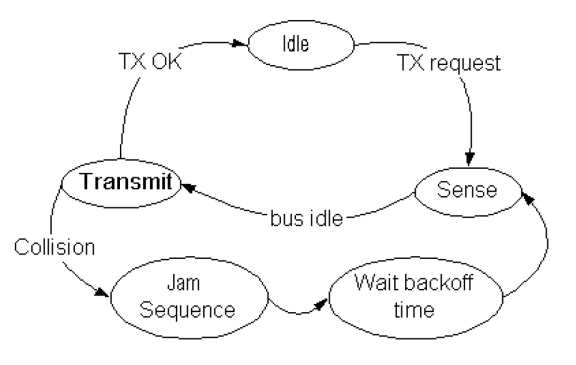
\includegraphics[width=\textwidth
]{images/csma-cd.png}
	\caption[Topologías de Red]{Topologías de Red}
	\label{fig:csma-cd}
\end{figure}

\subsubsection{Logical Link Control}
Es la subcapa de la capa de enlace que se encarga de procesar el paquete recibido en la capa MAC y enviarlo al proceso correspondiente en la capa de Red.

\subsection{Redes inalámbricas: Wi-Fi: IEEE 802.11b/g/n}
En las redes inalámbricas, los frames se mandan a través de ondas en una determinada frecuencia, que depende de la tecnología usada para transmitirlas. En este tipo de red, la intensidad de la señal disminuye con la distancia y tiene fuentes de ruidos más impredecibles que en medios guiados. Esto se traduce en una tasa de errores elevadas.

\subsubsection*{Spread Spectrum}
Esto sumado a que cualquier dispositivo cercarno puede conectarse a ellas, impulsaron el diseño de técnicas para aprovechar al máximo el ancho de banda de tal forma de proteger a la red de intrusos. Est técnica es llamada \textbf{Spread Spectrum}.

Esta técnica modula la señal usando una moduladora semi random compuesta de 1s y -1s conocida por los dispositivos de la red qur aplican a la señal que quieren enviar. Cuando la señal llega el receptor, este realiza el proceso inverso para conseguir la señal original.

Otra forma de realizar esto, es enviar la información transmitida en un rango de frecuencias que es cambiado varías veces durante el proceso de transmición. En este método, la información original se divide en partes más pequeñas usando un patron conocido solamente por el transmisor y el receptor.

\subsubsection{Carrier Sense Multiple Access / Collision Avoidance (CSMA/CA)}

Dado que las redes inalámbricas son un medio de broadcasting, los equipos de la red debe estar atentos a multiples transmiciones realizadas simultaneamente. 
A diferencia de los medios guiados, implementar una comunicación full-duplex sobre radio frecuencias es costoso por lo que se intenta evitar las colisiones en vez de resolverlas.

Para manejar esto, se utiliza el sistema CSMA descripto en la sección \ref{section::csma} pero adaptado a los problemas introducidosra minimizar la probabilidad de colisiones. Si durante este período, el medio se libera, el host puede transmitir una nueva trama. Si no, se vuelve a esperar un nuevo período de contentción. por el nuevo medio que es mucho más lento:

\subsubsection*{Colission Avoidance}
Antes de transmitir, una estación debe determinar el estado del medio. Si el canal no está ocupado, se realiza una espera adicional llamada \textbf{espaciado entre tramas} para asegurarnos de que no colisione.  Si durante esta espera, el medio no permanece libre, entonces se suspende la transmición hasta que se cumpla dicha condición.

Cuando la trama se transmitió, se espera recibir un ACK. Si esto no sucede, se asume que se perdió en una colisión y se retransmitirá la misma. 

Una vez que un host transmite una trama exitosamente, espera un \textbf{período de contención} (cuantificado por un back-off) para minimizar la probabilidad de colisiones. Si durante este período, el medio se libera, el host puede transmitir una nueva trama. Si no, se vuelve a esperar un nuevo período de contención.

Este método recién descripto es llamado \textbf{Distributed Coordination Function (DCF)} y es el método de acceso al medio más básico de 802.11.


\begin{figure}[H]
	\centering
	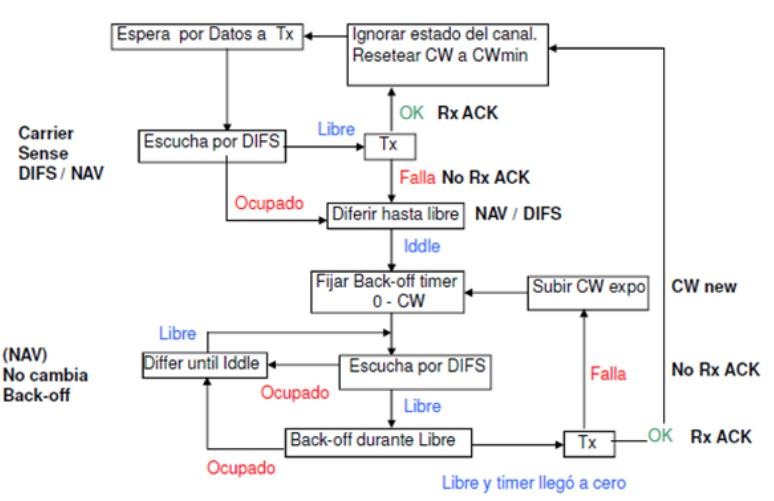
\includegraphics[width=\textwidth
]{images/wifi-estados.jpg}
	\caption[Máquina de estados de un host en una red Wifi]{Máquina de estados de un host en una red Wifi}
	\label{fig:wifi-estados}
\end{figure}

\subsubsection*{Problema de la estación oculta}
Supongamos que la computadora \(A\) comienza a transmitir a \(B\). 

Si \(C\) detecta el medio no escuchará a \(A\) porque está fuera de su alcance, y por lo tanto deducirá erroneamente que puede transmitir. Si lo hace, interferirá en \(B\) eliminando la trama de \(A\).

\begin{figure}[H]
	\centering
	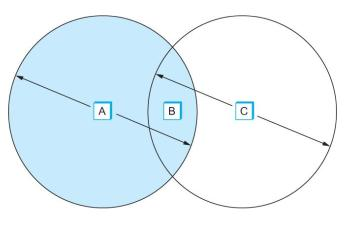
\includegraphics[width=0.5\textwidth
]{images/estacion-oculta.jpg}
	\caption[Problema de la estación oculta]{Problema de la estación oculta}
	\label{fig:estacion-oculta}
\end{figure}

\subsubsection*{Problema de la estación expuesta}
\begin{figure}[H]
	\centering
	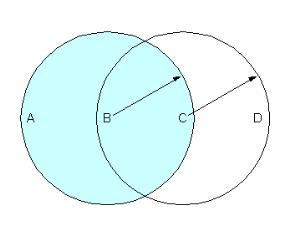
\includegraphics[width=0.5\textwidth
]{images/estacion-descubierta.jpg}
	\caption[Problema de la estación expuesta]{Problema de la estación expuesta}
	\label{fig:estacion-expuesta}
\end{figure}

Supongamos ahora que \(A\) está transmitiendo una tramba a \(B\). Supongamos ahora que \(C\) quiere transmitir a \(D\), cuando detecta al medio, escuhará una transmición y concluirá que no puede realizar su envio. Sin embargo, esa transmición causaría una mala recepción solo en la zona entre \(B\) y \(C\), en la que no está localizado ninguno de los receptores pretendidos.


\newpage
\part{Nivel de Red}
\begin{figure}[H]
	\centering
	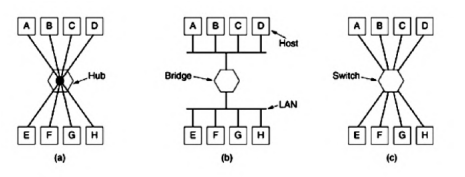
\includegraphics[width=\textwidth
]{images/topologias-red.png}
	\caption[Topologías de Red]{Topologías de Red}
	\label{fig:topologias-red}
\end{figure}
En la figura \ref{fig:topologias-red} se pueden ver tres tipos de LAN:
\begin{enumerate}[a)]
  \item En la primera vemos un conjunto de hosts conectados por un \textbf{hub}, esto es: Todos los hosts están conectado
  s entre sí como si los uniese un único cable. El \textbf{hub}, como los \textbf{repetidores} (amplificadores de señal), funcionan a nivel físico permitiendo agregar equipos a una red.
  \item En el segundo, un puente o \textbf{bridge}, separa en dos grupos los hosts de la red creando dos zonas independientes para la detección de colisiones. En este caso los hosts de un grupo podrán emitir sin tener que preocuparse por interferir con los hosts del otro grupo. Un paquete enviado la dirección de \textbf{broadcast}, alcanza a todos los hosts de la LAN.
  
  Puede interconectar, dos tipos de tecnología distintas (por ejemplo, ethernet y wifi). Por esta razón en la capa MAC, se agrega al header del paquete un campo que permite identificar el tipo de red del que viene. Cuando el bridge capta el paquete y se da cuenta que el host está en una red de distinto tipo, cambia el header para que matcheen y lo reenvía a través de la tecnología correspondiente
  \item Por último tenemos un conjunto de host conectados por un \textbf{switch}: Cada host se conecta con una conexión full-duplex al dispositivo, que se encarga de recibir todos los mensajes de un host y redireccionarlo al host correspondiente. En este tipo de redes se elimina la necesidad detectar colisiones y se pasa a necesitar un algoritmo que permita al switch realizar el dispatch de los mensajes de manera correcta.
  
  Tanto el switch como el bridge funciona a nivel capa de enlace. Se encargan de redireccionar los frames enviados a través de una LAN para que lleguen al dispositivo correspondiente.
\end{enumerate}

Agregamos un último dispositivo: El \textbf{router}, para conectar distintas redes a nivel red. Se encargán de buscar el camino que debe seguir para llegar a destino. Cuando una host envía decide enviar un paquete, lo encapsula en un frame que contiene el tipo de protocolo usado. Cuando el paquete llega el router, este se encarga de tomar el frame que le llego, desencapsular el paquete y guardarlo en un frame adecuado para que pueda ser interpretado por los dispositivos de la nueva ren en la que ingresa el frame.

\section{Switches}
En términos simples, un switch es un mecanismo que nos permite interconectar enlaces para formar una red más grande. Un switch es un dispositivo de múltiples entradas y salidas que transfiere paquetes desde una entrada a una o más salidas. El trabajo principal de un switch es recibir paquetes entrantes en uno de sus enlaces y transmitirlos en otro enlace. Esta función se denomina a veces conmutación (\textbf{switching}) o reenvío (\textbf{forwarding}).

Por lo tanto, un switch agrega la topología de estrella a la topología de enlace punto a punto. Una topología de estrella tiene varias propiedades atractivas:

\begin{itemize}
  \item Aunque un switch tiene un número fijo de entradas y salidas, lo que limita la cantidad de hosts que se pueden conectar a un solo switch, se pueden construir redes grandes interconectando varios switches.
  \item Podemos conectar switches entre sí y a hosts usando enlaces punto a punto, lo que típicamente significa que podemos construir redes de gran alcance geográfico.
  \item Agregar un nuevo host a la red conectándolo a un switch no necesariamente reduce el rendimiento de la red para otros hosts ya conectados.
\end{itemize}

Cada host en una red conmutada (Switched network) tiene su propio enlace al switch, por lo que puede ser completamente
posible que muchos hosts transmitan a la velocidad de enlace completa (ancho de banda),
siempre que el switch esté diseñado con suficiente capacidad agregada.

En general, las redes conmutadas son consideradas más escalables. 

Cuando un router recibe un paquete, busca, en el header del paquete, un identificador que usa para decidir a que puerto. Los detalles de como usa este identificador varían, pero hay dos enfoques comunes. El primero es el enfoque \textbf{datagrama} o \textbf{sin conexión}. El segundo es el enfoque de \textbf{circuito virtual} o \textbf{orientado a conexión}. Un tercer enfoque, el \textbf{enrutamiento de origen} (\textbf{source routing}), es menos común que estos otros dos, pero tiene algunas aplicaciones útiles.

Una cosa que es común a todas las redes es que necesitamos tener una forma de identificar los nodos con los que podremos comunicardos. En general, el identificador que se les asigna se llaman \textbf{direcciones}.

Otra cosa que debemos definir es como el router va a tomar la decisión de a que puerto enviar el paquete. Para esto, se define una \textbf{tabla de enrutamiento} que asocia una dirección de destino con un puerto de salida. En general, la tabla de enrutamiento se construye a partir de un algoritmo de enrutamiento.

\subsection{Redes de datagramas}
La idea detrás de los datagramas es increíblemente simple: Incluir en cada paquete suficiente información para permitir que cualquier switch decida cómo llevarlo a su destino. Es decir, cada paquete contiene la dirección de destino completa. Para decidir cómo reenviar un paquete, un switch consulta una tabla de forwarding (a veces llamada tabla de enrutamiento).

Las redes de datagramas tienen las siguientes características:
\begin{itemize}
  \item Un host puede enviar un paquete a cualquier destino en cualquier momento, ya que cualquier paquete que llegue a un switch puede ser reenviado inmediatamente (suponiendo una tabla de forwarding correctamente poblada). Por esta razón, las redes de datagramas a menudo se llaman sin conexión; esto contrasta con las redes orientadas a conexión en las que se debe establecer algún estado de conexión antes de que se envíe el primer paquete de datos.
  \item Cuando un host envía un paquete, no tiene forma de saber si la red es capaz de entregarlo o si el host de destino incluso está activo.
  \item Cada paquete se reenvía independientemente de los paquetes anteriores que podrían haberse enviado al mismo destino. Por lo tanto, dos paquetes sucesivos de host A a host B pueden seguir rutas completamente diferentes (quizás debido a un cambio en la tabla de forwarding en algún switch de la red).
  \item Una falla de switch o enlace puede no tener ningún efecto serio en la comunicación si es posible encontrar una ruta alternativa alrededor de la falla y actualizar la tabla de forwarding en consecuencia.
 \end{itemize}

\subsection{Circuitos virtuales}
Una segunda técnica para el conmutación de paquetes, que difiere significativamente del modelo de datagrama, usa el concepto de un \textbf{circuito virtual (VC)}.

Este enfoque, que también se conoce como \textbf{modelo orientado a conexión}, requiere configurar una conexión virtual desde el host de origen hasta el host de destino antes de que se envíe cualquier dato. Podemos pensar en esto como un proceso de dos etapas. La primera etapa es la "configuración de la conexión". El segundo es la transferencia de datos.

Durante el setup de la conexión, se establece un estado de conexión en cada uno de los switches entre los hosts de origen y destino. Una sola conexión consiste en una entrada en la "tabla VC" de cada switch que describe la conexión y que interfaces dentro de ese switch están involucradas en la misma. Entonces cada entrada de la tabla VC está formada por cuatro campos:

\begin{itemize}
  \item Un \textbf{identificador de circuito virtual (VCI)} que identifica de forma única la conexión en este switch y que se llevará dentro de la cabecera de los paquetes que pertenecen a esta conexión
  \item Una \textbf{interfaz de entrada} en la que el switch va a recibir los paquetes para este VC.
  \item Una \textbf{interfaz de salida} que se usará para reenviar los paquetes asociados al VC.
  \item El \textbf{VCI de salida} que se utilizará en el nuevo header de los paquetes que se forwardean.
 \end{itemize}
 
 La semántica de estas entradas es la siguiente: Si un paquete llega a la interfaz de entrada designada y ese paquete contiene el valor VCI designado en su encabezado, entonces ese paquete debe enviarse a la interfaz de salida especificada con el valor VCI de salida especificado (se remplaza el VCI de entrada en el header del paquete recibido por el nuevo antes de forwardearlo).

 La combinación del VCI de los paquetes a medida que se reciben en el switch y la interfaz de entrada identifican de forma única la conexión virtual. Puede haber muchas conexiones virtuales establecidas en un mismo switch al mismo tiempo. Además, los valores de VCI de entrada y salida generalmente no son los mismos. Por lo que el VCI no es un identificador de importancia global para la conexión; más bien, tiene importancia solo en un enlace dado.

 Cada vez que se crea una nueva conexión, debemos asignar un nuevo VCI para esa conexión en cada enlace que la conexión atravesará. También debemos asegurarnos de que el VCI elegido en un enlace determinado no esté actualmente en uso en ese enlace por alguna conexión existente.

\subsubsection{Creación de la conexión}
 Hay dos enfoques generales para establecer el estado de conexión: Uno es que un administrador de red configure el estado, en cuyo caso el circuito virtual es "permanente" (\textbf{Permanent Virtual Cirtcuit}). Este circuito también puede ser eliminado por el administrador. Alternativamente, un host puede enviar mensajes a la red para hacer que se establezca el estado. Esto se conoce como \textbf{señalización (signaling)}, y los circuitos virtuales resultantes se denominan conmutados (switched). La característica más importante de un \textbf{circuito virtual conmutado (SVC)} es que un host puede configurarlo y eliminarlo dinámicamente sin la participación de un administrador de red.

 Suponiendo que todos los nodos de la red saben la topología y la ubicación de cada nodo (esto se hace corriendo algoritmos de routing que vamos a ver más adelante), el algoritmo para crear una conexión es el siguiente: Si el host \(A\) quiere conectarse con el host \(B\) entonces:

 \begin{enumerate}
  \item \(A\) envía un paquete con un pedido de conexión a la red que contiene la dirección completa de \(B\).
  \item El paquete llega a un switch \(S_1\) que crea una entrada en su tabla de VC para la conexión registrando la interfaz desde la que le llegó el paquete y asignando el VCI de entrada. Luego busca en su tabla de forwarding cual es el próximo nodo que debe recibir el paquete.
  \item Cada switch al que le llega el paquete realiza la misma operación hasta que el mismo llega a \(B\).
  \item Finalmente, el pedido de conexión llega a \(B\) que decide si aceptar o no la conexion. Si lo hace, también asigna un valor VCI de entrada en su tabla de VC.
  \item Para completar, la conexión \(B\) envría un mensaje de aceptación que debe recorrer el camino establecido hasta \(A\) indicando a cada uno de los nodos cual es el VCI de salida que deben usar en cada paso.
  \item Cuando el último paquete llega a \(A\), cada switch tiene una entrada completa en su tabla de VC para la conexión.
  \end{enumerate}

Cuando el \(A\) ya no quiere enviar datos a \(B\), destruye la conexión enviando un mensaje de destrucción a \(S_1\). El switch elimina la entrada relevante de su tabla y reenvía el mensaje a los otros switches en el camino, que eliminan de manera similar las entradas apropiadas de sus tablas.

Hay varias cosas a tener en cuenta sobre el conmutación de circuitos virtuales:
\begin{itemize}
  \item \(A\) tiene que esperar a que la solicitud de conexión llegue al otro lado de la red y regrese antes de que pueda enviar su primer paquete de datos, hay al menos un tiempo de ida y vuelta (RTT) de retraso antes de que esto pueda suceder.
  \item Si bien la solicitud de conexión contiene la dirección completa del \(B\) (que puede ser bastante grande, ya que es un identificador global en la red), cada paquete de datos contiene solo un identificador pequeño, que es único solo en un enlace. Por lo tanto, la sobrecarga por paquete causada por el encabezado se reduce en relación con el modelo de datagrama.
  \item Si un switch o un enlace en una conexión falla, la conexión se rompe y se deberá establecer una nueva. Además, el circuito virtual roto debe ser desmantelado para liberar espacio de almacenamiento de tablas de los switches.
\end{itemize}

\subsubsection{Comparación con el modelo de datagrama}

Una de las ventajas de los circuitos virtuales es que para cuando el host recibe la señal de que puede enviar datos, sabe bastante sobre la red, por ejemplo, que realmente hay una ruta hacia el receptor y que el receptor está dispuesto y es capaz de recibir datos. También es posible asignar recursos al circuito virtual en el momento en que se establece.

En comparación, una red de datagramas no tiene una fase de establecimiento de conexión, y cada switch procesa cada paquete de forma independiente, lo que hace menos obvio cómo una red de datagramas asignaría recursos de manera significativa. En cambio, cada paquete que llega compite con todos los demás por el espacio del búfer. Si no hay búferes libres, el paquete entrante debe descartarse.

\subsection{Source Routing}
Un tercer enfoque al switching que no utiliza ni circuitos virtuales ni datagramas convencionales se conoce como \textbf{source routing}. En esta técnica,toda la información sobre la topología de la red que se requiere para conmutar un paquete es proporcionada por el host de origen. 

Es decir, el host de origen envía un paquete con un header que contiene toda la información necesaria para forwardear el paquete a su destino. El switch simplemente lee el header y lo reenvía al siguiente nodo. Una forma de hacer esto sería poner una lista ordenada de puertos de switch por el que se debe forwardear el paquete y rotar la lista para que el siguiente switch en el camino siempre esté al frente de la lista.

Hay varias cosas a tener en cuenta sobre este enfoque:

\begin{itemize}
  \item Asume que el host de origen sabe lo suficiente sobre la topología de la red para formar un encabezado que tenga todas las direcciones correctas para cada switch en el camino.
  \item  No podemos predecir cuán grande debe ser el encabezado, ya que debe poder contener una palabra de información para cada switch en el camino. Esto implica que probablemente sean de longitud variable sin límite superior, a menos que podamos predecir con absoluta certeza el número máximo de switches a través de los cuales un paquete necesitará pasar.
  \item Hay algunas variaciones en este enfoque. Por ejemplo, en lugar de rotar el encabezado, cada switch podría simplemente eliminar el primer elemento a medida que lo usa. La rotación tiene una ventaja sobre el stripping, sin embargo: el host B obtiene una copia del encabezado completo, lo que puede ayudarlo a descubrir cómo volver al host A. Otra alternativa es que el encabezado lleve un puntero al "próximo puerto" que debe ser usado, de modo que cada switch simplemente actualice el puntero en lugar de rotar el encabezado; esto puede ser más eficiente de implementar.
\end{itemize}

El source routing se puede usar tanto en redes de datagramas como en redes de circuitos virtuales. Por ejemplo, el Protocolo de Internet (IP), que es un protocolo de datagramas, incluye una opción de source routing que permite que se enrutan los paquetes seleccionados, mientras que la mayoría se conmutan como datagramas convencionales.

\subsection{Bridges and LAN Switches}
Comenzamos considerando una clase de switch que se usa para reenviar paquetes entre LAN (redes de área local) como Ethernets. Dichos switches a veces se conocen con el nombre obvio de \textbf{LAN switches}; históricamente, también se los ha denominado \textbf{bridges}, y se usan ampliamente en redes de campus y empresas.

Este tipo de nodo implementan completamente la detección de colisiones y los protocolos de acceso al medio en cada una de sus interfaces. Por lo tanto, las restricciones del protocolo sobre la distancia y número de hosts no se aplicarían al par de redes combinadas de esta manera. Este dispositivo opera en modo promiscuo, aceptando todos los tramas transmitidos en cualquiera de las redes y reenviándolos al otro.

Una colección de redes conectadas por uno o más bridges se dice que forman una \textbf{LAN extendida}.

\subsubsection{Learning Bridges}
La primera optimización que podemos hacer a un bridge es observar que no necesita reenviar todos los frames que recibe.

Para esto podemos hacer que cada bridge inspeccione la dirección de origen de todos los frames que recibe. Cuando un host \(A\) envía un frame a otro cualquiera, el bridge recibe este frame y registra el hecho de que se acaba de recibir un frame de \(A\) en tal interfaz \(I\). De esta manera, cuando reciba un mensaje que debe ser envíado a \(A\) lo manda directamente a la interfaz \(I\).

Cuando un bridge se inicia, esta tabla está vacía; las entradas se agregan con el tiempo. Además, se asocia un timeout con cada entrada para que el bridge la descarte después de cierto tiempo. Esto es para evitar que se mantenga una entrada que se quedó invalidada si un host, y como consecuencia, su dirección LAN, se mueve de una red a otra. Por lo tanto, esta tabla no es necesariamente completa. Si el bridge recibe un frame que está dirigido a un host que no está actualmente en la tabla reenvía el frame en todos los demás puertos.

\subsubsection{Spanning Tree Protocol}
La estrategia anterior funciona bien hasta que la LAN extendida tiene un ciclo, en cuyo caso falla miserablemente: los frames potencialmente se repiten a través de la LAN extendida eternamente.
\begin{figure}[H]
	\centering
	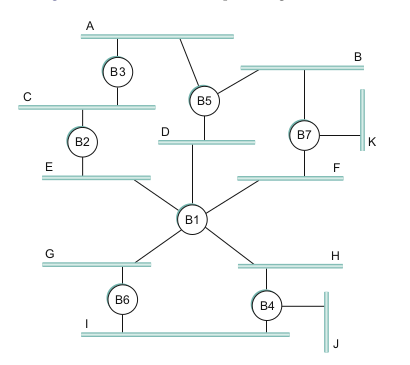
\includegraphics[width=0.5\textwidth
]{images/looped-network.png}
	\caption[Red con un ciclo]{Red con un ciclo}
	\label{fig:looped-network}
\end{figure}

Este problema se resuelve haciendo que los bridges ejecuten un algoritmo de \textbf{spaning tree} distribuido. Se piensa en la LAN extendida como si estuviera representada por un grafo que posiblemente tenga ciclos. Un spanning tree es un subgrafo de este grafo que cubre todos los vértices de la red pero no contiene ciclos. Es decir, un spanning tree mantiene todos los vértices del grafo original pero descarta algunas de las aristas.

El siguiente protocolo es utilizado por un conjunto de bridges para acordar el spanning tree para una LAN extendida en particular y funciona de la siguiente manera: Cada bridge tiene un identificador único; para nuestros propósitos, usamos las etiquetas \(B_1\), \(B_2\), \(B_3\), y así sucesivamente.

Los bridges tienen que intercambiar mensajes de configuración entre sí y luego decidir si son el root o un bridge designado en base a estos mensajes. Específicamente, estos mensajes contienen tres piezas de información:
\begin{enumerate}
  \item El ID del bridge que está enviando el mensaje
  \item El ID del bridge que es considerado el root (hasta el momento)
  \item La distancia, medida en saltos (hops), desde el bridge que envía hasta el root
\end{enumerate}

Inicialmente, cada bridge piensa que es la raíz, y por lo tanto envía un mensaje en cada uno de sus puertos identificándose como la raíz y dando una distancia de 0. 

Al recibir un mensaje sobre un puerto en particular, el bridge verifica si ese nuevo mensaje es mejor que el ya almacenado para ese puerto. Éste se considera mejor que la información actualmente grabada si se cumple alguna de las siguientes condiciones:
\begin{itemize}
  \item Identifica una raíz con un ID más pequeño.
  \item Identifica una raíz con un ID igual pero con una distancia más corta.
  \item El ID de la raíz y la distancia son iguales, pero el bridge que envía tiene un ID más pequeño.
\end{itemize}

Si el nuevo mensaje es mejor que la información actualmente grabada, el bridge descarta la información antigua y guarda la nueva. Sin embargo, primero agrega 1 a la distancia ya que el bridge está a un salto más lejos de la raíz que el bridge que envió el mensaje.

Cuando un bridge recibe un mensaje que indica que no es el bridge raíz, es decir, un mensaje de un bridge con un ID más pequeño, el mismo deja de generar mensajes por su cuenta y en su lugar solo reenvía los de otros bridges, después de agregar 1 al campo de distancia. Del mismo modo, cuando un bridge recibe un mensaje que indica que no es el bridge designado para ese puerto, el bridge deja de generara mensajes sobre ese puerto. Por lo tanto, cuando el sistema se estabiliza, solo el bridge raíz sigue generando mensajes, y los otros bridges están reenviando estos mensajes solo sobre los puertos para los que son el bridge designado. En este punto, se ha construido un spanning tree, y todos los bridges están de acuerdo en qué puertos se utilizan en el mismo. Solo esos puertos pueden usarse para reenviar paquetes de datos en la LAN extendida.

En cierto sentido, es eliminando puertos de la topología que la LAN extendida se reduce a un árbol acíclico. Incluso es posible que un bridge no participe en el reenvío de frames, lo que parece un poco extraño a primera vista. Sin embargo, el algoritmo es dinámico, lo que significa que los bridges siempre están preparados para reconfigurarse en un nuevo spanning tree si algún bridge falla, y por lo tanto, esos puertos y bridges no utilizados proporcionan la capacidad redundante necesaria para recuperarse de fallas.

Una cosa importante a tener en cuenta es que, aunque el algoritmo es capaz de reconfigurar el árbol de expansión cada vez que falla un bridge, no es capaz de reenviar frames por rutas alternativas para evitar un bridge congestionado.

Dado que el objetivo de un bridge es extender una LAN de manera transparente a través de múltiples redes, y dado que la mayoría de las LAN admiten tanto broadcast como multicast, los bridges también deben admitir estas dos características. Broadcast es simple: cada bridge reenvía un frame con una dirección de destino de broadcast en cada puerto activo que no sea el puerto por el que se recibió el frame.

Multicast se puede implementar de la misma manera, con cada host decidiendo por sí mismo si aceptar o no el mensaje.


El algoritmo del árbol de expansión se puede extender para podar las redes sobre las cuales no es necesario reenviar los frames multicast. Cada host que es miembro del grupo M debe periódicamente enviar un frame con la dirección para el grupo M en el campo de origen del encabezado del frame. Este frame tendría como dirección de destino la dirección multicast para los bridges. Sin embargo, esto es ineficiente, por lo que en general se usa la primera opción.

\subsubsection{Limitaciones de los bridges}
En cuanto a la escala, no es realista conectar más de unas pocas LAN mediante bridges. Una razón para esto es que el algoritmo del spanning tree escala linealmente. Una segunda razón es que los bridges reenvían todos los frames de broadcast.

Un enfoque para aumentar la escalabilidad de las LAN extendidas es la VLAN. Las VLAN permiten que una sola LAN extendida se divida en varias LAN separadas. A cada LAN virtual se le asigna un identificador (a veces llamado color), y los paquetes solo pueden viajar de un segmento a otro si ambos segmentos tienen el mismo identificador. Esto tiene el efecto de limitar el número de segmentos en una LAN extendida que recibirá cualquier paquete de broadcast.

En cuanto a la heterogeneidad, los bridges son bastante limitados en los tipos de redes que pueden interconectar. En particular, los bridges utilizan el header del frame de la red y, por lo tanto, solo pueden admitir redes que tengan exactamente el mismo formato para las direcciones. Por lo tanto, los bridges se pueden usar para conectar Ethernets a Ethernets, anillos de tokens a anillos de tokens y una red 802.11 a otra. También es posible poner un bridge entre, por ejemplo, un Ethernet y una red 802.11, ya que ambas redes admiten el mismo formato de dirección de 48 bits. Sin embargo, los bridges no se generalizan fácilmente a otros tipos de redes con diferentes formatos de direccionamiento.

\newpage
\section{IP}
Utilizamos el término \textbf{internet}, o a veces simplemente \textbf{internet} con una i minúscula, para referirnos a una colección arbitraria de redes interconectadas para proporcionar algún tipo de servicio de entrega de paquetes de host a host.

Una internet conecta diversas redes através de routers. Es fácil confundirse con la distinción entre bridges, switches y routers. Hay una buena razón para tal confusión, ya que en algún nivel todos reenvían mensajes de un enlace a otro. Una distinción que la gente hace se basa en la estratificación: los bridges son nodos de nivel de enlace (reenvían frames de un enlace a otro para implementar una LAN extendida), los switches son nodos de nivel de red (reenvían paquetes de un enlace a otro para implementar una red conmutada por paquetes) y los routers son nodos de nivel de internet (reenvían datagramas de una red a otra para implementar un internet).

El \textbf{Protocolo de Internet (Internet Protocol - IP)} es la herramienta clave utilizada hoy en día para construir internets escalables y heterogéneas.
La filosofía utilizada en la definición del modelo de servicio IP fue hacerlo poco exigente para que casi cualquier tecnología de red que pueda aparecer en una internet pueda proporcionar el servicio necesario.

El modelo de servicio IP puede pensarse en dos partes: un esquema de direccionamiento, que proporciona una forma de identificar todos los hosts en la internet, y un modelo de datagrama (sin conexión) de entrega de datos. Este modelo de servicio a veces se llama mejor esfuerzo (\textbf{best effort}) porque, aunque IP hace todo lo posible para entregar datagramas, no ofrece garantías.

Cada datagrama lleva suficiente información para permitir que la red reenvíe el paquete a su destino correcto; no es necesario ningún mecanismo de configuración previa para decirle a la red qué hacer cuando llega el paquete. Simplemente lo envía y la red hace todo lo posible para llevarlo al destino deseado. La parte de ``mejor esfuerzo" significa que si algo sale mal y el paquete se pierde, se corrompe, se entrega incorrectamente o de cualquier manera no llega a su destino previsto, la red no hace nada: hizo su mejor esfuerzo y eso es todo lo que tiene que hacer. No hace ningún intento de recuperarse del fallo. Esto a veces se llama un servicio no confiable.

La entrega de mejor esfuerzo no significa solo que los paquetes pueden perderse. A veces pueden entregarse fuera de orden, y a veces el mismo paquete puede entregarse más de una vez. Los protocolos de nivel superior o las aplicaciones que se ejecutan por encima de IP deben ser conscientes de todos estos posibles tipos de falla.

\subsection{Formato del paquete}
Una parte clave del modelo de servicio IP es el tipo de paquetes que se pueden transportar. El datagrama IP, como la mayoría de los paquetes, consiste en una cabecera seguida de un número de bytes de datos.


\begin{figure}[H]
	\centering
	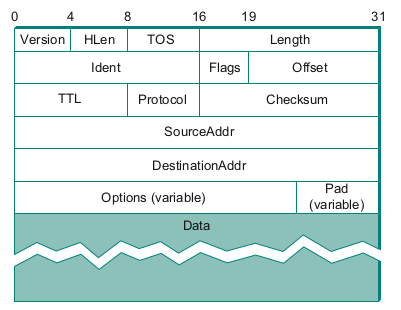
\includegraphics[width=0.5\textwidth
]{images/ip-frame.png}
	\caption[Paquete IP]{Paquete IP}
	\label{fig:ip-frame}
\end{figure}

El header del paquete consta de los siguientes campos:
\begin{itemize}
  \item El campo \textbf{Version} especifica la versión de IP. La versión actual de IP es 4, y a veces se llama IPv4. Colocar este campo justo al comienzo del datagrama facilita que todo lo demás en el formato del paquete se redefina en versiones posteriores.
  \item El campo \textbf{HLEN} especifica la longitud del encabezado en palabras de 32 bits. Cuando no hay opciones, lo que sucede en la mayoía de los casos, el encabezado tiene 5 palabras (20 bytes) de largo.
  \item El campo \textbf{TOS (tipo de servicio)} de 8 bits ha tenido una serie de definiciones diferentes a lo largo de los años, pero su función básica es permitir que los paquetes se traten de manera diferente según las necesidades de la aplicación.
  \item El campo \textbf{Length} (16 bits) contienen la longitud del datagrama, incluido el encabezado. A diferencia del campo HLen, el campo Longitud cuenta bytes en lugar de palabras. Por lo tanto, el tamaño máximo de un datagrama IP es de 65.535 bytes. Sin embargo, la red física a través de la cual se ejecuta IP puede no admitir paquetes tan largos. Por esta razón, IP admite un proceso de fragmentación y reensamblaje.
  \item Los campos \textbf{Ident}, \textbf{Flags} y \textbf{Offset} contienen información sobre la fragmentación, que se describe en la siguiente sección.
  \item El campo \textbf{TTL} es el tiempo de vida del paquete. La intención del campo es capturar paquetes que han estado dando vueltas en bucles de enrutamiento y descartarlos, en lugar de dejar que consuman recursos indefinidamente.

  Dado que no todos los enrutadores no tienen acceso a un reloj común, la mayoría de los enrutadores simplemente decrementaban el TTL en 1 a medida que envian el paquete. Por lo tanto, se convirtió más en un recuento de saltos que en un temporizador.

  Establecer este campo demasiado alto haría que los paquetes circulen bastante antes de ser descartados; Establecerlo demasiado bajo podría conllevar a que no lleguen a su destino. El valor 64 es el valor predeterminado actual.

  \item El campo \textbf{protocolo} es simplemente una clave de demultiplexión que identifica el protocolo de nivel superior al que se debe pasar este paquete IP. Hay valores definidos para TCP (Protocolo de control de transmisión - 6), UDP (Protocolo de datagramas de usuario - 17) y muchos otros protocolos.
  
  \item El campo \textbf{Checksum} es un campo de detección de errores de 16 bits que cubre tanto el encabezado como los datos. Sirve para detectar errores, no así para corregirlos. Por lo tanto, si el host detecta un error en el paquete, lo descarta.
  \item El campo \textbf{SourceAddr} es la dirección completa del host que envía el paquete. Es necesaria para permitir que los destinatarios decidan si desean aceptar el paquete y para permitirles responder.
  \item El campo \textbf{DestinationAddr} es la dirección completa del host que debe recibir el paquete.  Es la clave para la entrega de datagramas.
  \item Finalmente, puede haber una serie de opciones al final del encabezado. La presencia o ausencia de opciones se puede determinar examinando el campo HLen. Si bien las opciones se usan con bastante poca frecuencia, una implementación IP completa debe poder procesarlas todas.
\end{itemize}

\subsection{Fragmentación y reensambe}
Cada tipo de red tiene una \textbf{unidad de transmisión máxima (Maximum Transmission Unit - MTU)}, que es el datagrama IP más grande que puede transportar en un frame.

Cuando un host envía un datagrama IP, puede elegir cualquier tamaño que desee. Una opción razonable es el MTU de la red a la que está directamente conectado. En este caso, la fragmentación solo será necesaria si la ruta hacia el destino incluye una red con un MTU más pequeño. Si el protocolo de transporte que se encuentra en la parte superior de IP le da un paquete más grande que el MTU local, entonces el host de origen debe fragmentarlo.

Para permitir que estos fragmentos se vuelvan a ensamblar en el host de recepción, todos llevan el mismo identificador en el campo \texttt{Ident}. Este identificador es elegido por el host de envío y se elige de tal forma que sea único entre todos los datagramas que puedan llegar al destino desde esta fuente durante un período de tiempo razonable. Dado que todos los fragmentos del datagrama original contienen este identificador, el host de reensambe podrá reconocer aquellos fragmentos que van juntos. Si no llegan todos los fragmentos al host de recepción, el host abandona el proceso de reensamble y descarta los fragmentos que llegaron. IP no intenta recuperarse de fragmentos faltantes.

Supongamos que hay que fragmentar un mensaje recibido, entonces se divide el datgrama en paquetes I más pequeños y en el primer paquete se establece el bit \texttt{M} en el campo \texttt{Flags}, lo que significa que hay más fragmentos por seguir, y establece el \texttt{Offset} en 0, ya que este fragmento contiene la primera parte del datagrama original.

Cuando el host recibe todos los fragmentso, usa el offset de cada paquete para reordenarlos y luego los concatena para formar el datagrama completo. El reensamblaje se realiza en el host receptor y no en cada enrutador.

\subsection{Direcciones globales}
Las direcciones Ethernet son globalmente únicas pero eso solo no es suficiente para un esquema de direccionamiento en una gran internet. Las direcciones Ethernet también son planas, lo que significa que no tienen estructura y proporcionan muy pocas pistas para los protocolos de enrutamiento.

En contraste, las direcciones IP son jerárquicas: Están compuestas de varias partes que corresponden a algún tipo de jerarquía en la internet. Específicamente, las direcciones IP consisten en dos partes denominadas parte de red y parte de host. La parte de red de una dirección IP identifica la red a la que está conectado el host;  todos los hosts conectados a la misma red tienen la misma parte de red en su dirección IP. La parte del host identifica de forma única cada host en esa red en particular.

Los router   que se conectan a dos o más redes necesitan tener una dirección en cada red, una para cada interfaz. Por lo tanto, teniendo en cuenta que un enrutador podría implementarse como un host con dos interfaces de red, es más preciso pensar en las direcciones IP como pertenecientes a interfaces que a hosts.

La clase de una dirección IP se identifica en los bits más significativos. Si el primer bit es 0, es una dirección de clase A. Si el primer bit es 1 y el segundo es 0, es una dirección de clase B. Si los dos primeros bits son 1 y el tercero es 0, es una dirección de clase C. 

\begin{figure}[H]
	\centering
	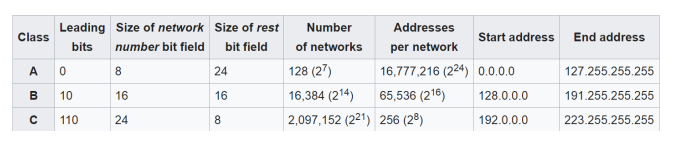
\includegraphics[width=\textwidth
]{images/ip-address-classes.png}
	\caption[Clases de direcciones IP]{Clases de direcciones IP}
	\label{fig:ip-address-classes}
\end{figure}

Por convención, las direcciones IP se escriben como cuatro enteros decimales separados por puntos. Cada entero representa el valor decimal contenido en 1 byte de la dirección, comenzando por el bit más significativo.

\subsubsection{Forwarding de datagramas en IP}
Un datagrama se envía desde un host de origen a un host de destino, posiblemente pasando por varios routers en el camino. Cualquier nodo, ya sea un host o un enrutador, primero intenta establecer si está conectado a la misma red física que el destino. Para hacer esto, compara la parte de red de la dirección de destino con la parte de red de la dirección de cada una de sus interfaces de red.

Si hay alguna una coincidencia significa que el destino se encuentra en la misma red física que la interfaz y el paquete se puede entregar directamente a través de esa red.

Si el nodo no está conectado a la misma red física que el nodo de destino entonces debe elegir a quien debe pasar el datagrama para acercarlo a su destino. En general, cada nodo tendrá una \textbf{tabla de forwarding} que enumera los posibles routers a los que pueda reenviar el paquete por lo que debe elegir el mejor, o al menos uno que tenga una posibilidad razonable de realizar esta tareas. El router que termina eligiendo se conoce como \textbf{next hop}. Cada fila de la tabla es un par \(<NetworkNum, NextHop>\).

En caso de no encontrar una opción que considere viable, el paquete se envía a un router default almacenado en la tabla.

\subsection{Subnetting}
\textbf{Subnetting} proporciona un primer paso para reducir el número total de números de red que se asignan a una tabla de forwarding. La idea es tomar un solo número de red IP y asignar las direcciones IP con ese número de red a varias redes físicas, que ahora se denominan subredes. Varias cosas deben hacerse para que esto funcione. Primero, las subredes deben estar cerca unas de otras. Esto se debe a que en un punto distante de Internet, todas parecerán una sola red, teniendo solo un número de red entre ellas. Esto significa que un enrutador solo podrá seleccionar una ruta para llegar a cualquiera de las subredes, por lo que es mejor que todas estén en la misma dirección general.

Se agrega a la identificación de un host una \textbf{máscara de subred} que permitirá identificar la red a la que pertenece un host. De esta manera, podrá haber varios host con el mismo número de red pero pertenecen a distintas redes físicas. 

Cuando el host quiere enviar un paquete a una cierta dirección IP, lo primero que hace es realizar un AND bit a bit entre su propia máscara de subred y la dirección IP de destino. Si el resultado es igual al número de subred del host de envío, entonces sabe que el host de destino está en la misma subred y el paquete se puede entregar directamente sobre la subred.

Si los resultados no son iguales, el paquete debe enviarse a un enrutador para que se reenvíe a otra subred.

La tabla de forwarding de un enrutador también cambia ligeramente cuando introducimos el subnetting. Recordemos que anteriormente teníamos una tabla de forwarding que consistía en entradas de la forma \(<NetworkNum, NextHop>\). Para soportar el subnetting, la tabla ahora debe tener entradas de la forma \(<SubnetNumber, SubnetMask, NextHop>\). Para encontrar la entrada correcta en la tabla, el enrutador realiza un AND bit a bit entre la dirección de destino del paquete y la SubnetMask para cada entrada; si el resultado coincide con el SubnetNumber de la entrada, entonces esta es la entrada correcta para usar, y reenvía el paquete al enrutador indicado.

\subsubsection{Direcciones sin clases}
El subnetting tiene un contraparte, a veces llamado supernetting, pero más a menudo llamado \textbf{Classless Interdomain Routing} o \textbf{CIDR}, pronunciado "cider". CIDR lleva la idea de subnetting a su conclusión lógica al eliminar las clases de direcciones por completo. 

El subnetting solo nos permite dividir una dirección de clase entre múltiples subredes, mientras que CIDR nos permite fusionar varias direcciones de clase en una sola "supernet" y lo hace de una manera que evita que el sistema de enrutamiento se sobrecargue.


CIDR trata de equilibrar el deseo de minimizar el número de rutas que un enrutador necesita conocer contra la necesidad de asignar direcciones de manera eficiente. Para hacer esto, CIDR nos ayuda a agregar rutas. Es decir, nos permite usar una sola entrada en una tabla de forwarding para decirnos cómo llegar a muchas redes diferentes. Como se señaló anteriormente, lo hace rompiendo los límites rígidos entre las clases de direcciones.

CIDR requiere un nuevo tipo de notación para representar los números de red, o prefijos como se los conoce, porque los prefijos pueden tener cualquier longitud. La convención es colocar un /X después del prefijo, donde X es la longitud del prefijo en bits.

Si asignamos prefijos a los clientes de tal manera que muchas redes de clientes diferentes conectadas a la red del proveedor compartan un prefijo de dirección común y más corto, entonces podemos obtener una mayor agregación de rutas.

\subsubsection*{IP Forwarding y CIDR}
Usar CIDR significa que los prefijos pueden tener cualquier longitud, desde 2 hasta 32 bits. Además, a veces es posible tener prefijos en la tabla de forwarding que "se superponen", en el sentido de que algunas direcciones pueden coincidir con más de un prefijo.

La regla en este caso se basa en el principio de "coincidencia más larga"; es decir, el paquete coincide con el prefijo más largo.

El algoritmo para encontrar eficientemente la coincidencia más larga entre una dirección IP y los prefijos de longitud variable en una tabla de forwarding utiliza un enfoque conocido como árbol PATRICIA.

\subsection{Addressing Translation (ARP)}
Uno de los principales problemas que falta resolver es que los datagramas IP contienen direcciones IP, pero el hardware de interfaz física en el host o enrutador al que desea enviar el datagrama solo comprende el esquema de direccionamiento de esa red en particular. Por lo tanto, necesitamos traducir la dirección IP a una dirección de nivel de enlace que tenga sentido en esta red (por ejemplo, una dirección Ethernet de 48 bits). Luego podemos encapsular el datagrama IP dentro de un frame que contenga esa dirección de nivel de enlace y enviarlo al destino final o a un enrutador que prometa reenviar el datagrama hacia el destino final.

Esto se puede lograr utilizando el Protocolo de Resolución de Direcciones (ARP). El objetivo de ARP es permitir que cada host en una red construya una tabla de asignaciones entre direcciones IP y direcciones de nivel de enlace. Dado que estas asignaciones pueden cambiar con el tiempo, las entradas se eliminan periódicamente. Esto sucede en el orden de cada 15 minutos. El conjunto de asignaciones almacenadas actualmente en un host se conoce como caché ARP o tabla ARP.


ARP aprovecha el hecho de que muchas tecnologías de red de nivel de enlace, como Ethernet, admiten broadcasting. Si un host desea enviar un datagrama IP a otro host (o a un enrutador) que sabe que está en la misma red, primero verifica si hay un mapeo en la caché. Si no se encuentra ningún mapeo, debe invocar el Protocolo de resolución de direcciones en la red. Lo hace transmitiendo una consulta ARP en la red. Esta consulta contiene la dirección IP de destino. Cada host recibe la consulta y verifica si coincide con su dirección IP. Si coincide, el host envía un mensaje de respuesta que contiene su dirección de nivel de enlace de regreso al originador de la consulta. El originador agrega la información contenida en esta respuesta a su tabla ARP.

La consulta también incluye la dirección IP y la dirección de nivel de enlace del host que envía. De esta manera, el host de destino puede aprender las direcciones de nivel de enlace y de IP del remitente y colocar esa información en su tabla ARP si es que ya no la tenía guardada.  Si el host ya tiene una entrada para ese host en su tabla, aumenta el time to live de esta entrada para que dure más tiempo.

El formato del paquete ARP para mapeos de direcciones IP a Ethernet contiene:
\begin{itemize}
    \item Un campo \textbf{HardwareType}, que especifica el tipo de red física.
    \item Un campo \textbf{ProtocolType}, que especifica el protocolo de capa superior
    \item Campos \textbf{HLen} ("longitud de dirección de hardware") y \textbf{PLen} ("longitud de protocolo"), que especifican la longitud de la dirección de capa de enlace y la dirección de protocolo de capa superior, respectivamente
    \item Un campo \textbf{Operation}, que especifica si se trata de una solicitud o una respuesta
    \item Las direcciones de hardware (Ethernet) y protocolo (IP) de origen y destino
\end{itemize}

\subsection{Host Configuration (DHPC)}
Las direcciones IP, no solo deben ser únicas en una interred determinada, sino que también deben reflejar la estructura de la misma. Como se señaló anteriormente, contienen una parte de red y una parte de host, y la parte de red debe ser la misma para todos los hosts en la misma red. Por lo tanto, no es posible configurar la dirección IP una vez en un host cuando se fabrica, ya que eso implicaría que el fabricante sabía qué hosts iban a terminar en qué redes, y significaría que un host, una vez conectado a una red, nunca podría moverse a otra. Por esta razón, las direcciones IP deben ser reconfigurables.

El método principal de configuración utiliza un protocolo conocido como \textbf{Protocolo de configuración dinámica de host (DHCP)}. DHCP se basa en la existencia de un servidor DHCP que es responsable de proporcionar información de configuración a los hosts. Existe al menos un servidor DHCP por dominio administrativo.

El servidor DHCP mantiene un grupo de direcciones disponibles que entrega a los hosts a pedido. Esto reduce considerablemente la cantidad de configuración que debe realizar un administrador, ya que ahora solo es necesario asignar un rango de direcciones IP (todas con el mismo número de red) a cada red.

Para contactar a un servidor DHCP, un host recién iniciado o conectado envía un mensaje \textbf{DHCPDISCOVER} a una dirección IP especial (255.255.255.255) que es una dirección de broadcast en IP. Esto significa que será recibido por todos los hosts y enrutadores en esa red. (Los enrutadores no reenvían dichos paquetes a otras redes, evitando la difusión a toda Internet). En el caso más simple, uno de estos nodos es el servidor DHCP para la red. El servidor respondería entonces al host que generó el mensaje de descubrimiento.

Sin embargo, no es realmente deseable requerir un servidor DHCP en cada red, porque esto implica una gran cantidad de servidores que deben configurarse correctamente y de manera consistente. Por lo tanto, DHCP utiliza el concepto de un agente de retransmisión. Hay al menos un agente de retransmisión en cada red, y se configura con solo una pieza de información: la dirección IP del servidor DHCP. Cuando un agente de retransmisión recibe un mensaje DHCPDISCOVER, lo envía en unicast al servidor DHCP y espera la respuesta, que luego enviará al cliente solicitante.

El mensaje se envía realmente utilizando un protocolo llamado \textbf{Protocolo de Datagrama de Usuario (UDP)} que se ejecuta sobre IP.

En el caso en que DHCP asigne dinámicamente direcciones IP a los hosts, no pueden mantener las direcciones indefinidamente, ya que esto eventualmente causaría que el servidor agote su pool de direcciones. Al mismo tiempo, no se puede depender de que un host devuelva su dirección, ya que podría haberse bloqueado, desconectado de la red o apagado. Por lo tanto, DHCP permite que las direcciones se asignen por un período de tiempo determinado. Una vez que la asignación expire, el servidor es libre de devolver esa dirección a su pool. Un host con una dirección asignada necesita renovar el arriendo periódicamente si todavía está conectado a la red y funciona correctamente.

\subsection{Error Reporting (ICMP)}
IP siempre se configura con un protocolo complementario conocido como \textbf{Protocolo de mensajes de control de Internet (ICMP)}. Este protocolo define una colección de mensajes de error que se envían al host de origen cada vez que un enrutador o host no puede procesar un datagrama IP correctamente.

ICMP también define mensajes de control que un enrutador puede enviar de vuelta a un host de origen. Uno de los mensajes de control más útiles, llamado ICMP-Redirect, le dice al host de origen que hay una mejor ruta hacia el destino.

\subsection{Virtual Networks and Tunneling}

Las empresas con varios sitios tienden a construir redes privadas alquilando lineas de compañias electrónicas para interconectarlos. En estas redes, la comunicación se restringe a los sitios de la corporación, lo cual es deseable por razones de seguridad. Para hacer una red privada virtual, las lineas de transmisión alquiladas - que no son compartidas con otras corporaciones - serían reemplazadas por algún tipo de red compartida. Un circuito virtual (VC) es un reemplazo razonable para una linea alquilada porque aún provee una conexión lógica punto a punto entre los sitios de la corporación.

También es posible proporcionar una función similar utilizando una red IP, una interred, para proporcionar la conectividad. Sin embargo, no podemos simplemente conectar los sitios de las diversas corporaciones a una sola interred porque eso proporcionaría conectividad entre la corporación X y la corporación Y, lo que deseamos evitar. Para resolver este problema, necesitamos introducir un nuevo concepto, el \textbf{túnel IP}.

Podemos pensar en un túnel IP como un enlace virtual punto a punto entre un par de nodos que están separados por un número arbitrario de redes. El enlace virtual se crea dentro de un enrutador \(R_1\) en la entrada del túnel al proporcionarle la dirección IP del enrutador \(R_2\) en el otro extremo del túnel. Cada vez que \(R_1\) desea enviar un paquete por este enlace virtual, encapsula el paquete dentro de un datagrama IP. La dirección de destino en el encabezado IP es la dirección de \(R_2\), mientras que la dirección de origen es la de \(R_1\).

Una vez que el paquete sale de \(R_1\), parece al resto del mundo como un paquete IP normal destinado a \(R_2\), y se reenvía en consecuencia. Todos los enrutadores en la interred lo reenvían utilizando medios normales, hasta que llega a \(R_2\). Cuando \(R_2\) recibe el paquete, encuentra que lleva su propia dirección, por lo que elimina el encabezado IP y mira la carga útil del paquete. Lo que encuentra es un paquete IP interno cuya dirección de destino está en una red interna. \(R_2\) ahora procesa este paquete como cualquier otro paquete IP que recibe. Dado que \(R_2\) está directamente conectado a esta red, reenvía el paquete a esa red.

Este mecanismo tiene sus desventajas. Una es que aumenta la longitud de los paquetes; esto podría representar una pérdida significativa de ancho de banda para paquetes cortos. Los paquetes más largos pueden estar sujetos a fragmentación, que tiene su propio conjunto de inconvenientes. También puede haber implicaciones de rendimiento para los enrutadores en cada extremo del túnel, ya que necesitan hacer más trabajo que el reenvío normal al agregar y eliminar el encabezado del túnel.

Finalmente, existe un costo de administración para la entidad administrativa que es responsable de configurar los túneles y asegurarse de que sean manejados correctamente por los protocolos de enrutamiento.

\newpage
\section{Ruteo interno y externo}
El problema de ruteo es como los switches y routers adquieren la información en sus tablas de forwarding.

Si bien los términos \textbf{tabla de forwarding} y \textbf{tabla de ruteo} son a veces usados indistintamente, haremos una distinción entre ellos aquí. La \textbf{tabla de forwarding} es usada cuando un paquete está siendo reenviado y por lo tanto debe contener suficiente información para realizar la función de forwarding. Esto significa que una fila en la tabla de forwarding contiene el mapeo de un prefijo de red a una interfaz de salida y alguna información MAC, como la dirección Ethernet del siguiente salto. La \textbf{tabla de ruteo}, por otro lado, es la tabla construida por los algoritmos de ruteo como un precursor para construir la tabla de forwarding. Generalmente contiene mapeos de prefijos de red a siguientes saltos. También puede contener información sobre cómo se aprendió esta información, para que el enrutador pueda decidir cuándo debe descartarla.

Los protocolos descritos en esta sección se conocen colectivamente como \textbf{protocolos de enrutamiento intradominio}, o Interior Gateway Protocols (IGP). Para comprender estos términos, debemos definir un dominio de enrutamiento: es una internet en la que todos los enrutadores están bajo el mismo control administrativo.

\subsection{La red como un grafo}
El ruteo es, en esencia, un problema de teoría de grafos. Los nodos del grafo pueden ser hosts, switches, routers o redes. Para nuestra discusión inicial, nos centraremos en el caso en que los nodos son enrutadores. Las aristas del grafo corresponden a los enlaces de red. Cada arista tiene un costo asociado, que da alguna indicación de la facilidad con la que se puede enviar tráfico a través de ese enlace.

Para resolver el problema de ruteo debemos encontrar el camino de menor costo entre dos nodos, donde el costo de un camino es igual a la suma de los costos de todas las aristas que componen el camino.

Los protocolos de ruteo proporcionan una forma distribuida y dinámica de resolver este problema en presencia de fallas de enlace y nodo y cambios en los costos de los enlaces.

Asumiendo que ya sabemos los costos de cada enlace vamos a ver dos algoritmos distribuidos que nos permiten crear la tabla de ruteo: \textbf{Distance Vector} y \textbf{Link State}.

\subsection{Distance Vector}
Cada nodo construye un vector que contiene las distancias (costos) a todos los otros nodos y distribuye ese vector a sus vecinos inmediatos. La suposición inicial para el ruteo vectorial de distancia es que cada nodo conoce el costo del enlace a cada uno de sus vecinos directamente conectados. Estos costos pueden ser provistos cuando el router es configurado por un administrador de red. Un enlace que está caído es asignado un costo infinito.

Inicialmente, cada nodo establece un costo de 1 a sus vecinos directamente conectados y \(\infty\) a todos los demás nodos.

En el siguiente paso, cada nodo envía un mensaje a sus vecinos directamente conectados indicando su lista personal de distancias.

Cuando un nodo recibe un vector de distancias, compara las distancias recibidas con las que tiene almacenadas en su tabla de ruteo. Si la distancia recibida es menor que la que tiene almacenada, la actualiza y envía su propio vector de distancias a sus vecinos.
\begin{figure}[H]
	\centering
	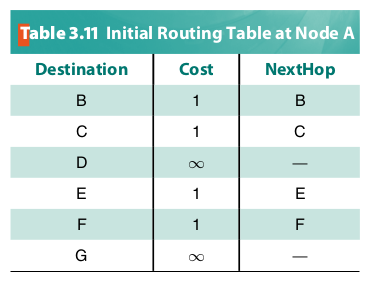
\includegraphics[width=0.5\textwidth
]{images/distance-vector-routing-table.png}
	\caption[Ejemplo tabla de ruteo]{Ejemplo tabla de ruteo}
	\label{fig:distance-vector-routing-table}
\end{figure}

En ausencia de cambios en la topología, solo se necesitan unos pocos intercambios de información entre vecinos antes de que cada nodo tenga una tabla de enrutamiento completa. El proceso de obtener información de enrutamiento consistente para todos los nodos se llama convergencia.

Los algoritmos distribuidos como este permiten que todos los nodos en la red se adapten automáticamente a los cambios en la topología de la misma. No se requiere intervención manual por parte de un administrador de red.

\subsubsection{Comportamiento ante fallas}
Hay dos circunstancias en las cuales un nodo dado decide enviar una actualización de enrutamiento a sus vecinos: 

\begin{itemize}
  \item Una \textbf{actualización periódica} se envía cada cierto tiempo, incluso si no ha cambiado nada. Esto sirve para que los otros nodos sepan que este nodo todavía está en funcionamiento. También se asegura de que sigan recibiendo información que puedan necesitar si sus rutas actuales se vuelven inviables. La frecuencia de estas actualizaciones periódicas varía de un protocolo a otro, pero generalmente está en el orden de varios segundos a varios minutos.
  \item Cuando un enlace o nodo falla (\textbf{triggered update}). Los nodos que notan esta situación primero envían nuevas listas de distancias a sus vecinos, y normalmente el sistema se estabiliza bastante rápido a un nuevo estado. 
\end{itemize}

Dependiendo el protocolo, la detección de una falla se puede dar de dos formas:
\begin{itemize}
  \item Un nodo prueba continuamente el enlace a otro nodo enviando un paquete de control y viendo si recibe un acuse de recibo.
  \item Un nodo determina que el enlace (o el nodo en el otro extremo del enlace) está inactivo si no recibe la actualización de enrutamiento periódica esperada durante los últimos ciclos de actualización.
\end{itemize}

\subsubsection{Conteo hasta el infinito}

Sucede cuando se cae un nodo o enlace y los nodos restantes no se dan cuenta de que el nodo o enlace ha fallado y hay nodos en la red que no alcanzan a enterarse de esto antes de que otro y deciden usarlos para crear el nuevo camino que los lleve al nodo caído. 
\begin{figure}[H]
	\centering
	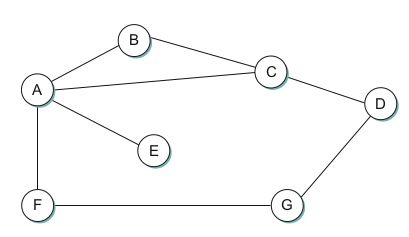
\includegraphics[width=0.5\textwidth
]{images/network-graph.png}
	\caption[Grafo de una red]{Grafo de una red}
	\label{fig:network-graph}
\end{figure}

Supongamos que se cae el enlace de \(A\) a \(E\) en la red mostrada arriba, supongamos se produce la ronda de periodic updates. Todos los nodos, envían su vector de distancias a sus vecinos. Puede suceder lo siguiente:
\begin{enumerate}
  \item  \(A\) anuncia una distancia de \(\infty\) a \(E\).
  \item \(B\) recibe de \(A\): \(\langle E,\infty\rangle\).
  \item \(B\) decide que a partir de ahora puede llegar a \(E\) usando \(C\) con una distancia de \(3\) y reenvía su vector de distancias antes de recibir el vector de distancias modificado de \(C\).
  \item \(A\) recibe el mensaje de \(B\) y decide que puede llegar a \(E\) usando \(B\) con una distancia de \(4\) y reenvía su vector de distancias.
  \item Cuando \(C\) reciba este paquete, sabe que puede usar \(A\) para recibir paquetes de \(E\) con una distancia de \(5\).
\end{enumerate}

Este ciclo se detiene solo cuando las distancias alcanzan algún número lo suficientemente grande como para considerarse infinito. Mientras tanto, ninguno de los nodos sabe realmente que \(E\) es inalcanzable, y las tablas de enrutamiento de la red no se estabilizan.

Hay varias soluciones parciales a este problema:
\begin{itemize}
  \item La primera es poner un número de distancia máximo pequeño como aproximación al infinito. Esto al menos limita la cantidad de tiempo que se tarda en contar al infinito. Por supuesto, también podría presentar un problema si nuestra red creciera hasta el punto en que algunos nodos estuvieran separados por más de la distancia máxima que habiamos definido.
  \item Otra técnica se llama \textbf{Split Horizon}: La idea es que cuando un nodo envía una actualización de enrutamiento a sus vecinos, no envía esas rutas que aprendió de cada vecino de vuelta a ese vecino. Por ejemplo, si \(B\) tiene la ruta \(\langle E, 2, A\rangle\) en su tabla, entonces sabe que debe haber aprendido esta ruta de \(A\), por lo que cada vez que \(B\) envía una actualización de enrutamiento a \(A\), no incluye la ruta \(\langle E, 2\rangle\) en esa actualización.
  \item Una variación más fuerte, llamada \textbf{Split Horizon with posion reverse}, vuelve a evniar la ruta \(A\) pero con una distancia de \(\infty\). Esto le dice a \(A\) que no puede llegar a \(E\) a través de \(B\).
\end{itemize}

El problema con estas técnicas que solo funcionan para loops que involucran dos nodos, se necesitan tomar decisiones más drásticas para loops más grandes. Se podría haber hecho que \(B\) y \(C\) esperen una cantidad determinada de tiempo antes de reenviar las nuevas rutas. Desafortunadamente, este enfoque retrasa la convergencia del protocolo; la velocidad de convergencia es una de las principales ventajas de su competidor: \textbf{Link-State Routing}.

\subsubsection*{Ruting Information Protocol (RIP)}
Uno de los protocolos de enrutamiento más utilizados en las redes IP es el Protocolo de Información de Enrutamiento (RIP).

En una internetwork, el objetivo de los enrutadores es aprender a reenviar paquetes a varias redes. Por lo tanto, en lugar de anunciar el costo de llegar a otros enrutadores, los enrutadores anuncian el costo de llegar a las redes.

RIP es una implementación bastante sencilla del algoritmo de Vector Distance Routing. Los enrutadores que ejecutan RIP envían sus anuncios cada 30 segundos.

Un enrutador también envía un mensaje de actualización cada vez que una actualización de otro enrutador hace que cambie su tabla de enrutamiento. Un punto de interés es que admite múltiples familias de direcciones, no solo IP. RIP versión 2 (RIPv2) también introdujo las máscaras de subred mientras que RIP versión 1 funcionaba con las direcciones de clase antigua de IP.

\subsection{Link State Routing}
Link State Routing es la segunda clase principal de protocolo de enrutamiento intradominio. Los supuestos iniciales para este protocolo son bastante similares a los del enrutamiento por distance vector. Se supone que cada nodo es capaz de descubrir el estado del enlace a sus vecinos y el costo de cada enlace.

Cada nodo sabe cómo llegar a sus vecinos directamente conectados, y si nos aseguramos de que la totalidad de este conocimiento se difunda a cada nodo, entonces cada nodo tendrá suficiente conocimiento de la red para construir un mapa completo. Esta es una condición suficiente (aunque no necesaria) para encontrar el camino más corto a cualquier punto de la red. Los protocolos de link state routing se basan en dos mecanismos: la difusión confiable de la información de estado de enlace y el cálculo de rutas a partir de la suma de todo el conocimiento acumulado por este algoritmo.

\subsubsection{Reliable flooding}
La inundación confiable (reliable flooding) es el proceso de asegurarse de que todos los nodos que participan en el protocolo de enrutamiento obtengan una copia de la información de estado de enlace de todos los demás nodos. Como sugiere el término inundación, la idea es que un nodo envíe su información de estado de enlace en todas sus conexiones directas; cada nodo que recibe esta información luego la reenvía en todas sus conexiones. Este proceso continúa hasta que la información ha llegado a todos los nodos de la red.

Más precisamente, cada nodo crea un paquete de actualización, también llamado paquete de estado de enlace (Link State Packet, LSP), que contiene la siguiente información:

\begin{itemize}
  \item El ID del nodo que creó el LSP.
  \item Una lista de vecinos directamente conectados de ese nodo, con el costo del enlace a cada uno.
  \item Un número de secuencia
  \item Un tiempo de vida (Time To Live - TTL) para este paquete
\end{itemize}

Los primeros dos elementos son necesarios para permitir el cálculo de rutas; los dos últimos se utilizan para que el proceso de inundación del paquete a todos los nodos sea confiable. La confiabilidad incluye asegurarse de tener la copia más reciente de la información, ya que puede haber múltiples LSP contradictorios de un mismo nodo circulando en la red.

Veamos como el proceso de flooding: 
\begin{itemize}
  \item Supongamos que un nodo \(A\) crea un LSP y lo envía a todos sus vecinos.
  \item Un nodo \(B\) que recibe una copia de un LSP que se originó en \(A\).
  \item \(B\) compara el número de secuencia del LSP que acaba de recibir con el número de secuencia del LSP que ya tiene almacenado para \(A\). Si el nuevo LSP tiene un número de secuencia más grande, se asume que es el más reciente, y ese LSP se almacena, reemplazando al antiguo. Un número de secuencia más pequeño (o igual) implicaría un LSP más antiguo (o no más nuevo) que el almacenado, por lo que se descartaría y no sería necesario tomar más medidas.
  \item Si el LSP recibido fue el más nuevo, X envía una copia de ese LSP a todos sus vecinos, excepto al vecino del que se acaba de recibir el LSP.
\end{itemize}

El hecho de que el LSP no se envíe de vuelta al nodo desde el que se recibió ayuda a poner fin a la inundación de un LSP. Dado que \(B\) pasa el LSP a todos sus vecinos, que luego hacen lo mismo, la copia más reciente del LSP eventualmente llega a todos los nodos.

Al igual que en RIP, cada nodo genera LSP bajo dos circunstancias:
\begin{itemize}
  \item La expiración de un LSP, debido a que su TTL ha llegado a cero.
  \item Un cambio en la topología de la red. Sin embargo, la única razón basada en la topología para que un nodo genere un LSP es si uno de sus enlaces conectados directamente o vecinos inmediatos ha fallado.
\end{itemize}

La falla de un enlace puede detectarse en algunos casos por el protocolo de capa de enlace. La desaparición de un vecino o la pérdida de conectividad con ese vecino se puede detectar mediante paquetes periódicos "hello". Cada nodo envía estos a sus vecinos inmediatos a intervalos definidos. Si pasa suficiente tiempo sin recibir un "hello" de un vecino, el enlace a ese vecino se declarará inactivo y se generará un nuevo LSP para reflejar este hecho.

\subsubsection{Consideraciones de diseño}
Uno de los objetivos de diseño más importantes de la inundación en este protocolo es que la información más reciente debe inundarse a todos los nodos lo más rápido posible, mientras que la información antigua debe eliminarse de la red. Además, es deseable minimizar la cantidad total de tráfico de enrutamiento que se envía por la red; después de todo, esto es solo una sobrecarga desde la perspectiva de aquellos que realmente usan la red para sus aplicaciones. 

Una forma facil de reducir el overhead es generar LSPs solo cuando es necesario. Esto puede hacerse usando TTLs muy largos, a menudo del orden de horas. Dado que el protocolo de inundación es realmente confiable cuando cambia la topología, es seguro asumir que no es necesario emitir mensajes de que algo ha cambiado.

El algoritmo de enrutamiento de estado de enlace tiene muchas propiedades agradables: se ha demostrado que se estabiliza rápidamente, no genera mucho tráfico y responde rápidamente a los cambios de topología o fallas de los nodos. Por otro lado, la cantidad de información almacenada en cada nodo (un LSP para cada nodo en la red) puede ser bastante grande.

\subsubsection{Número de secuencia}
Cada vez que un nodo genera un nuevo LSP, lo incrementa en 1. A diferencia de la mayoría de los números de secuencia utilizados en otros protocolos, no se espera que estos se reseteen, por lo que el campo debe ser bastante grande (digamos, 64 bits). 

Si un nodo se apaga y luego vuelve a encenderse, comienza con un número de secuencia de 0. Si el nodo estuvo inactivo durante mucho tiempo, todos los LSP antiguos para ese nodo habrán expirado; de lo contrario, eventualmente recibirá una copia de su propio LSP con un número de secuencia más alto, que luego puede incrementar y usar como su propio número de secuencia. Esto asegurará que su nuevo LSP reemplace cualquiera de sus viejos LSP que hayan quedado desde antes de que el nodo se apagara.

\subsubsection{Time To Live}
Se usa para asegurarse de que la información de estado de enlace antigua se elimine eventualmente de la red. Un nodo siempre decrementa el TTL de un LSP recién recibido antes de inundarlo a sus vecinos. También "envejece" el LSP mientras se almacena en el nodo. Cuando el TTL llega a 0, el nodo vuelve a inundar el LSP con un TTL de 0, que es interpretado por todos los nodos de la red como una señal para eliminar ese LSP.

\subsubsection{Calculo de rutas}
Una vez que un nodo determinado tiene una copia del LSP de todos los nodos de la red, puede calcular un mapa completo para la topología de la red, y a partir de este mapa puede decidir la mejor ruta para cada destino.

En la práctica, cada switch calcula su tabla de enrutamiento directamente a partir de los LSP que ha recopilado utilizando una versión del algoritmo de Dijkstra llamado algoritmo de \textbf{forward searching}. Específicamente, cada switch mantiene dos listas, conocidas como \texttt{Tentative} y \texttt{Confirmed}. Cada una de estas listas contiene un conjunto de entradas de la forma \\ \(\langle \texttt{Destino}, \texttt{Costo}, \texttt{NextHop}\rangle\). El algoritmo funciona de la siguiente manera:
\begin{enumerate}
  \item Se inicializa la lista \texttt{Confirmed} con una entrada para el propio nodo; esta entrada tiene un costo de 0.
  \item Para el nodo recién agregado a la lista \texttt{Confirmed} en el paso anterior,  se selecciona su LSP y lo marcamos como \texttt{Next}.
  \item Para cada vecino (\texttt{Neighbor}) de \texttt{Next}, se calcula el costo (\textbf{Costo}) para llegar a este Vecino como la suma del costo desde mí mismo hasta \texttt{Next} y desde \texttt{Next} hasta \texttt{Neighbor}.
  \begin{enumerate}
    \item Si \texttt{Neighbor} no está actualmente en la lista \texttt{Confirmed}  ni en la lista \texttt{Tentative}, agregue \(\langle\texttt{Vecino}, \texttt{Costo}, \texttt{NextHop}\rangle\) a la lista \texttt{Tentative}, donde \texttt{NextHop} es el nodo al que necesito ir para llegar a \texttt{Next}.
    \item Si \texttt{Neighbor} está actualmente en la lista \texttt{Tentative}, y el \texttt{Costo} es menor que el costo actualmente listado para \texttt{Neighbor}, reemplace la entrada actual con \\ \(\langle\texttt{Neighbor}, \texttt{Costo}, \texttt{NextHop}\rangle\), donde \texttt{NextHop} es el nodo al que necesito ir para llegar a \texttt{Next}.
  \end{enumerate}
  \item Si \texttt{Tentative} está vacía, ya están todas las rutas calculadas. De lo contrario, se elije la entrada con el costo más bajo, se la mueve \texttt{Confirmed} y se vuelve a hacer todo el proceso desde el paso 2.
\end{enumerate}

\subsubsection{Open Shortest Path First Protocol (OSPF)}
OSPF agrega una cantidad considerable de características al algoritmo básico de link-state descrito anteriormente:

\begin{itemize}
  \item \textbf{Autenticación de mensajes de enrutamiento}: una característica de los algoritmos de enrutamiento distribuido es que dispersan información de un nodo a muchos, y toda la red puede verse afectada por la información incorrecta de un nodo. Por esta razón, es una buena idea asegurarse de que todos los nodos que participan en el protocolo puedan confiar en ellos. La autenticación de mensajes de enrutamiento ayuda a lograr esto.
  \item \textbf{Jerarquía}: Es una de las herramientas fundamentales utilizadas para hacer que los sistemas sean más escalables. OSPF introduce otra capa de jerarquía en el enrutamiento al permitir que un dominio se divida en áreas. Esto significa que un enrutador dentro de un dominio no necesariamente necesita saber cómo llegar a cada red dentro de ese dominio, puede ser capaz de salir adelante sabiendo cómo llegar a la zona correcta. Por lo tanto, hay una reducción en la cantidad de información que debe transmitirse y almacenarse en cada nodo.
  \item \textbf{Balanceo de carga}: OSPF permite que varias rutas al mismo lugar se asignen el mismo costo y hará que el tráfico se distribuya uniformemente entre ellas, lo que permite un mejor uso de la capacidad de red disponible.
  \item Todo el paquete, excepto los datos de autenticación, está protegido por una suma de comprobación de 16 bits utilizando el mismo algoritmo que la cabecera IP.
  \item 
\end{itemize}

De los cinco tipos de mensajes OSPF, el tipo 1 es el mensaje "hola", que un enrutador envía a sus pares para notificarles que todavía está vivo y conectado como se describe anteriormente. Los tipos restantes se utilizan para solicitar, enviar y confirmar la recepción de mensajes de estado de enlace. El bloque de construcción básico de los mensajes de estado de enlace en OSPF es el anuncio de estado de enlace (Link Stata advertisement - LSA). Un mensaje puede llegar a contener varios LSA.

Específicamente, un enrutador que ejecuta OSPF puede generar LSPs que anuncian una o más de las redes que están directamente conectadas a ese enrutador. Además, un enrutador que está conectado a otro enrutador por algún enlace debe anunciar el costo de llegar a ese enrutador a través del enlace. Estos dos tipos de anuncios son necesarios para permitir que todos los enrutadores en un dominio determinen el costo de llegar a todas las redes en ese dominio y el siguiente salto apropiado para cada red.

\subsection{Métricas}
Una de las métricas más basicas, que es bastante razonable y muy simple, es asignar un costo de 1 a todos los enlaces: la ruta de menor costo será la que tenga menos saltos. Sin embargo, dicho enfoque tiene varias desventajas:
\begin{itemize}
  \item No distingue entre enlaces en función de la latencia,
  \item No distingue entre rutas en función de la capacidad,
  \item No distingue entre enlaces en función de su carga actual, lo que hace imposible evitarlos si están sobrecargados.
\end{itemize}

\subsubsection{ARPANET}
La métrica de enrutamiento original de ARPANET medía la cantidad de paquetes que se encolaban esperando ser transmitidos en cada enlace. Sin embargo, dado que la longitud de la cola es una medida artificial de la carga, cuando un enlace tiene un costo demasiado alto, los paquetes se terminan enviando hacia la cola más corta en lugar de hacia el destino.

\subsubsection{ARPANET v2}
Una segunda versión del algoritmo de ruteo ARPANET, a veces llamado el nuevo mecanismo de ruteo, tuvo en cuenta tanto el ancho de banda del enlace como la latencia y utilizó el retraso, en lugar de la longitud de la cola, como medida de carga. Esto se hizo de la siguiente manera. Primero, cada paquete entrante se marca con la hora de llegada al enrutador (\(ArrivalTime\)) y se registra su hora de salida del enrutador (\(DepartTime\)). En segundo lugar, cuando se recibió el ACK de nivel de enlace desde el otro lado, el nodo calculó el retraso para ese paquete como 

\[Delay = (DepartTime - ArrivalTime) + TransmissionTime + Latency\]

donde \(TransmissionTime\) y \(Latency\) se definieron estáticamente para el enlace y representan el ancho de banda y la latencia del mismo, respectivamente.

Si el ACK no llegó, sino que en su lugar el paquete agotó el tiempo de espera, entonces \(DepartTime\) se restablece al momento en que se retransmitió el paquete. En este caso, \(DepartTime - ArrivalTime\) captura la confiabilidad del enlace: cuanto más frecuente sea la retransmisión de paquetes, menos confiable será el enlace y más querremos evitarlo. Finalmente, el peso asignado a cada enlace se deriva del retraso promedio experimentado por los paquetes enviados recientemente a través de ese enlace.

Sin embargo, bajo una carga pesada, un enlace congestionado comienza a anunciar un costo muy alto. Esto causa que todo el tráfico se moviera fuera de ese enlace, dejándolo inactivo, por lo que luego anunciaría un costo bajo, atrayendo de vuelta todo el tráfico, y así sucesivamente. El efecto de esta inestabilidad es que, bajo una carga pesada, muchos enlaces pasarían mucho tiempo inactivos, que es lo último que desea bajo una carga pesada.

\subsubsection{Revised ARPANET Routing Metric}
Un tercer enfoque, llamado "métrica de enrutamiento ARPANET revisada", abordó estos problemas. Los principales cambios fueron comprimir el rango dinámico de la métrica considerablemente, tener en cuenta el tipo de enlace y suavizar la variación de la métrica con el tiempo.

La suavización se logró usando los siguientes mecanismos:
\begin{itemize}
  \item La medición del retraso se transformó en una utilización del enlace, y este número se promedió con la última utilización informada para suprimir los cambios repentinos.
  \item Se impuso un límite estricto sobre cuánto podría cambiar la métrica de un ciclo de medición al siguiente. Al suavizar los cambios en el costo, la probabilidad de que todos los nodos abandonen una ruta a la vez se reduce en gran medida.
\end{itemize} 

\newpage
\part{Nivel de Transporte}
\section{Protocolos End-to-End}
Los procesos del nivel de aplicación que usan los servicios de la capa de transporte esperan que proporcione ciertos requisitos:
\begin{itemize}
  \item Garantizar la entrega de mensajes
  \item Entregar mensajes en el mismo orden en que se envían
  \item Entregar a lo sumo una copia de cada mensaje
  \item Soportar mensajes arbitrariamente grandes
  \item Soportar sincronización entre el emisor y el receptor
  \item Permitir al receptor aplicar control de flujo al emisor
  \item Soportar múltiples procesos de aplicación en cada host  
\end{itemize}
\subsection{UDP}
El protocolo de transporte más simple posible es uno que extiende el servicio de entrega de host a host de la red subyacente en un servicio de comunicación de proceso a proceso. Es probable que haya muchos procesos en ejecución en cualquier host dado, por lo que el protocolo necesita agregar un nivel de demultiplexión, lo que permite que varios procesos de aplicación en cada host compartan la red. Aparte de este requisito, el protocolo de transporte no agrega ninguna otra funcionalidad al servicio de mejor esfuerzo proporcionado por la red subyacente. El \textbf{Protocolo de Datagramas de Usuario} (User Datagrama Procol - UDP) de Internet es un ejemplo de este tipo de protocolo de transporte.

Los procesos se identifican indirectamente entre sí utilizando un localizador abstracto, generalmente llamado puerto (\textbf{port}).

La cabecera de un protocolo de extremo a extremo que implementa esta función de demultiplexación típicamente contiene un identificador (puerto) tanto para el remitente (origen) como para el receptor (destino) del mensaje. Es decir, un proceso es realmente identificado por un puerto en algún host en particular, un par \(\langle host, puerto\rangle\).

\subsubsection{Comunicación entre procesos}
\begin{figure}[H]
	\centering
	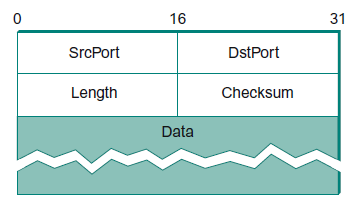
\includegraphics[width=0.5\textwidth
]{images/udp-header.png}
	\caption[Formate de Header para UDP]{Formate de Header para UDP}
	\label{fig:udp-header}
\end{figure}
Típicamente, un proceso cliente inicia un intercambio de mensajes con un proceso servidor. Una vez que el mensaje inicial esrecibido, el servidor conoce el puerto del cliente (del campo \textbf{SrcPrt} contenido en la cabecera del mensaje) y puede responderle. 

Los servidores, esperan recibir mensajes en puertos bien conocidos (\textbf{well-known ports}). Algunos ejemplos:
\begin{itemize}
  \item Los servidores de nombres de dominio (DNS) recibe mensajes en el puerto 53.
  \item El servicio de correo escucha mensajes en el puerto 25.
  \item Unix acepta mensajes en el puerto 517
\end{itemize}

Este mapeo se publica periódicamente en un RFC y está disponible en la mayoría de los sistemas Unix en el archivo /etc/services. A veces, un puerto bien conocido es solo el punto de partida para la comunicación: el cliente y el servidor usan el puerto bien conocido para acordar algún otro puerto que usarán para la comunicación posterior, dejando el puerto bien conocido libre para otros clientes.

\subsubsection{Manejo de mensajes}
\begin{figure}[H]
	\centering
	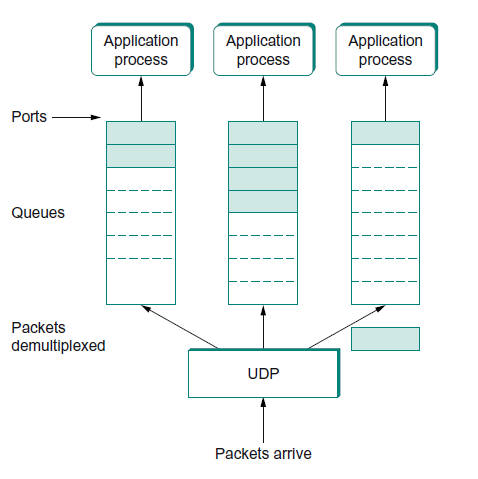
\includegraphics[width=0.5\textwidth
]{images/udp-message-queue.png}
	\caption[Cola de mensajes de UDP]{Cola de mensajes de UDP}
	\label{fig:udp-message-queue}
\end{figure}

Cuando llega un mensaje, el protocolo lo agrega al final de la cola. Si la cola está llena, el mensaje se descarta. No hay mecanismo de control de flujo en UDP para decirle al remitente que se ralentice. Cuando un proceso de aplicación desea recibir un mensaje, se elimina uno de la parte delantera de la cola. Si la cola está vacía, el proceso se bloquea hasta que haya un mensaje disponible.

Finalmente, aunque UDP no implementa el control de flujo o la entrega confiable / ordenada, también garantiza la corrección del mensaje mediante el uso de un cheksum. El mismo  toma como entrada el encabezado UDP, el contenido del cuerpo del mensaje y algo llamado \textbf{pseudoencabezado}. El pseudoencabezado consiste en tres campos del encabezado IP: número de protocolo, dirección IP de origen y dirección IP de destino, más el campo de longitud UDP. La motivación detrás de tener el pseudoencabezado es verificar que este mensaje se haya entregado entre los dos puntos finales correctos.

\subsection{Transmission Control Protocol (TCP)}
TCP garantiza la entrega confiable y en orden de un flujo de bytes. Es un protocolo full-duplex, lo que significa que cada conexión TCP admite dos flujos de bytes simulteanos en dirección opuesta. También incluye un mecanismo de control de flujo para cada uno de ellos, lo que permite al receptor limitar la cantidad de datos que el remitente puede transmitir en un momento dado. La idea de este mecanismo es limitar la velocidad a la que TCP envía datos, no por el bien de evitar que el remitente sobrecargue al receptor, sino para evitar que el remitente sobrecargue la red. Finalmente, al igual que UDP, TCP admite un mecanismo de demultiplexación que permite que varios programas de aplicación en cualquier host dado mantengan una conversación simultánea con sus pares. 

\subsubsection{Sliding Window en TCP}
TCP usa el algoritmo de ventana deslizante para asegurar la entrega confiable de los mensajes. Aunque este es el mismo algoritmo básico que vimos en la Sección \ref{sec:ventana-deslizante}, debido a que TCP se ejecuta a través de Internet en lugar de una conexión punto a punto, hay muchas diferencias importantes:
\begin{itemize}
  \item TCP admite conexiones lógicas entre procesos que se ejecutan entre dos computadoras cualquieras conectadas al Internet por lo que necesita una fase explícita de establecimiento de conexión durante la cual ambos nodos acurdan intercambiar información entre sí. Esto genera un estado compartido entre ellos que se usa para comenzar el algoritmo de ventana deslizante y que debe ser liberado cuando la conexión se cierra por lo que TCP también tiene una fase explícita de desmontaje de la conexión.
  \item Mientras que un solo enlace físico que siempre conecta las mismas dos computadoras tiene un tiempo de Round-Trip Time (RTT), las conexiones TCP probablemente tendrán tiempos de ida y vuelta diferentes dependiendo de la distancia entre ellas, la carga de la red, etc. Las variaciones en el RTT incluso son posibles durante una sola conexión TCP que dura solo unos minutos. Osea que el algoritmo de ventana deslizante debe tener un mecanismo retransmisiones con tiempos de espera adaptativos.
  \item Los paquetes pueden reordenarse a medida que cruzan el Internet. Los paquetes que están ligeramente desordenados no causan un problema ya que el algoritmo de ventana deslizante puede reordenar los paquetes correctamente usando el número de secuencia. El verdadero problema es cuán desordenados pueden estar los paquetes o, dicho de otra manera, cuán tarde puede llegar un paquete a su destino. En el peor de los casos, un paquete puede retrasarse en Internet hasta que expire el campo de tiempo de vida (TTL) de IP, momento en el cual el paquete se descarta (y, por lo tanto, no hay peligro de que llegue tarde). Sabiendo que IP descarta los paquetes después de que expire su TTL, TCP asume que cada paquete tiene un tiempo de vida máximo. El tiempo de vida exacto, conocido como tiempo de vida máximo del segmento (Maximum Segment Life - MSL), es una opción de ingeniería. La implicación es significativa: TCP tiene que estar preparado para que los paquetes muy antiguos aparezcan repentinamente en el receptor, lo que podría confundir el algoritmo de ventana deslizante.
  \item Casi cualquier tipo de computadora puede estar conectada a Internet, lo que hace que la cantidad de recursos dedicados a cualquier conexión TCP sea muy variable, especialmente considerando que cualquier host puede potencialmente admitir cientos de conexiones TCP al mismo tiempo. Esto significa que TCP debe incluir un mecanismo que cada lado usa para "aprender" qué recursos (por ejemplo, cuánto espacio de búfer) el otro lado puede aplicar a la conexión. Este es el problema de control de flujo.
\end{itemize}

\subsubsection{Formato de los segmentos}
TCP es un protocolo orientado a bytes, lo que significa que el remitente escribe bytes en una conexión TCP y el receptor lee bytes de la conexión TCP. Aunque "flujo de bytes" describe el servicio que el protocolo ofrece a los procesos de aplicación, el mismo no transmite bytes individuales a través de Internet. En cambio, en el host de origen, almacena en un búfer suficientes bytes del proceso de envío para llenar un paquete de tamaño razonable y luego envía este paquete a su par en el host de destino. En el host de destino, TCP vacía el contenido del paquete en un búfer de recepción, y el proceso de recepción lee de este búfer a su gusto.

Los paquetes intercambiados entre pares TCP se llaman segmentos, ya que cada uno lleva un segmento del flujo de bytes. Cada segmento contiene el siguiente encabezado:

\begin{figure}[H]
	\centering
	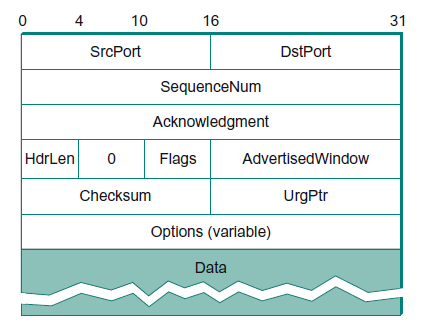
\includegraphics[width=0.5\textwidth
]{images/tcp-header.png}
	\caption[Encabezado de un paquete TCP]{Encabezado de un paquete TCP}
	\label{fig:tcp-header}
\end{figure}

\begin{itemize}
  \item \texttt{SrcPort} y \texttt{DstPort} identifican los puertos de origen y destino, respectivamente, al igual que en UDP. Estos dos campos, más las direcciones IP de origen y destino, se combinan para identificar de manera única cada conexión TCP. Es decir, la clave de demultiplexación de TCP está dada por la tupla de 4 elementos \texttt{SrcPort}, \texttt{SrcIPAddr}, \texttt{DstPort}, \texttt{DstIPAddr}.
  \item \texttt{Acknowledgment}, \texttt{SequenceNum} y \texttt{AdvertisedWindow} están involucrados en el algoritmo de ventana deslizante de TCP.
  \item \texttt{Flags} es un campo de 6 bits que se utiliza para transmitir información de control. Incluye los siguientes bits:
  \begin{itemize}
    \item \texttt{ACK} se establece cada vez que el campo \texttt{Acknowledgment} es válido, lo que implica que el receptor debe prestar atención a él. 
    \item\texttt{URG} significa que este segmento contiene datos urgentes. Cuando se establece este indicador, el segemento contiene datos urgentes desde el byte 0 hasta el byte \texttt{UrgPtr} 
    \item\texttt{PUSH} significa que el remitente invocó la operación de empuje, esto indica que el receptor debe poder leer la información contenida en el segmento apenas llegue.
    \item \texttt{RESET} significa que el receptor se ha confundido, por ejemplo, porque recibió un segmento que no esperaba recibir, por lo que desea abortar la conexión.
  \end{itemize}
  \item \texttt{Checksum} se usa exactamente de la misma manera que para UDP: se calcula sobre el encabezado TCP, los datos TCP y el pseudoencabezado, que está compuesto por los campos de dirección de origen, dirección de destino y longitud del encabezado IP. El checksum es obligatorio para TCP tanto en IPv4 como en IPv6. 
  \item \texttt{HdrLen} indica la longitud del encabezado TCP en palabras de 32 bits. Este campo también se conoce como el campo \texttt{Offset}, ya que mide el desplazamiento desde el inicio del paquete hasta el inicio de los datos.
\end{itemize}

\subsubsection{Establecimiento de una conexión TCP}
Una conexión TCP comienza con un cliente (caller) haciendo una apertura activa a un servidor (callee). Suponiendo que el servidor hubiera hecho una apertura pasiva anteriormente, los dos lados se involucran en un intercambio de mensajes para establecer la conexión. Solo después de que finalice esta fase, los dos lados pueden comenzar a enviar datos. De manera similar, tan pronto como un participante haya terminado de enviar datos, cierra una dirección de la conexión, lo que hace que TCP inicie una ronda de mensajes de terminación de conexión.

\subsubsection*{3-Way Handshake}
\begin{figure}[H]
	\centering
	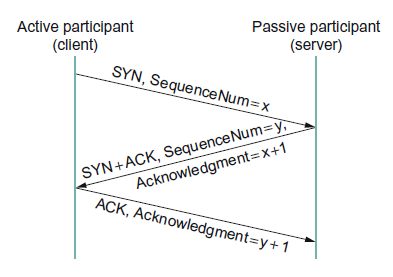
\includegraphics[width=0.5\textwidth
]{images/three-way-handshake.png}
	\caption[Intercambio de mensajes para 3-Way Handshake]{Intercambio de mensajes para 3-Way Handshake}
	\label{fig:three-way-handshake}
\end{figure}
El algoritmo utilizado por TCP para establecer y terminar una conexión se llama handshake de tres vías (Three Way Handshake).

Dos computadoras que quieran inicializar una conexión, deben acordar los números de secuencia de inicio que las dos partes planean usar para sus respectivos flujos de bytes. Primero, el cliente (el participante activo) envía un segmento al servidor (el participante pasivo) indicando el número de secuencia inicial que planea usar (\texttt{FLAG = SYN, SequenceNum = x}). El servidor responde con un solo segmento que reconoce el número de secuencia del cliente (\texttt{FLAG = ACK, Ack = x + 1}) y establece su propio número de secuencia de inicio (\texttt{Flags = SYN + ACK, SequenceNum = y}). Finalmente, el cliente responde con un tercer segmento que reconoce el número de secuencia del servidor (\texttt{Flags = ACK, Ack = y + 1}). La razón por la cual cada lado reconoce un número de secuencia que es uno más grande que el enviado es que el campo de reconocimiento realmente identifica el "siguiente número de secuencia esperado", reconociendo implícitamente todos los números de secuencia anteriores. Aunque no se muestra en esta línea de tiempo, se programa un temporizador para cada uno de los dos primeros segmentos, y si no se recibe la respuesta esperada, el segmento se retransmite.

\subsubsection{Diagrama de transición de estados de TCP}
Todas las conexiones comienzan en el estado CLOSED. A medida que la conexión avanza, la conexión se mueve de un estado a otro de acuerdo con los arcos. Cada arco está etiquetado con una etiqueta de la forma evento / acción.

\begin{figure}[H]
	\centering
	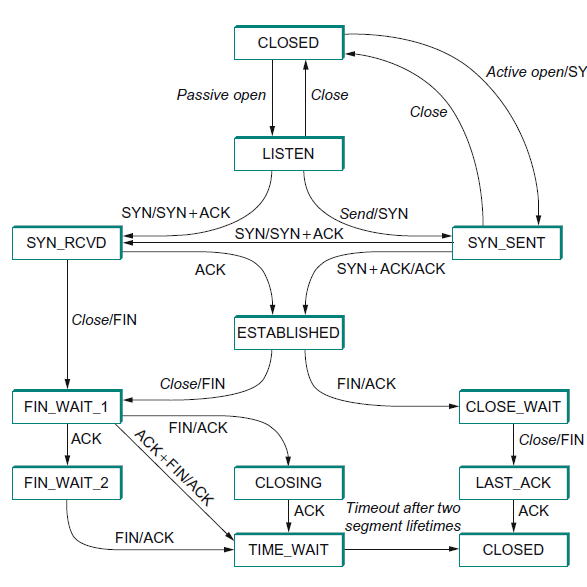
\includegraphics[width=0.5\textwidth
]{images/tcp-state-transitions.png}
	\caption[Transiciones de estado TCP]{Transiciones de estado TCP}
	\label{fig:tcp-state-transitions}
\end{figure}

\paragraph{Inicio de conexión:}Al abrir una conexión, el servidor primero invoca una operación de apertura pasiva, lo que hace que TCP se mueva al estado \texttt{LISTEN}. En algún momento posterior, el cliente realiza una apertura activa, lo que hace que su extremo de la conexión envíe un segmento \texttt{SYN} al servidor y se mueva al estado \texttt{SYN SENT}. Cuando el segmento \texttt{SYN} llega al servidor, se mueve al estado \texttt{SYN RCVD} y responde con un segmento \texttt{SYN + ACK}. La llegada de este segmento hace que el cliente se mueva al estado \texttt{ESTABLISHED} y envíe un \texttt{ACK} de vuelta al servidor. Cuando llega este \texttt{ACK}, el servidor finalmente se mueve al estado \texttt{ESTABLISHED}.

Si el \texttt{ACK} del cliente al servidor se pierde, la conexión aún funciona correctamente. Esto se debe a que el lado del cliente ya está en el estado \texttt{ESTABLISHED}, por lo que el proceso de aplicación local puede comenzar a enviar datos al otro extremo. Cada uno de estos segmentos de datos tendrá el indicador \texttt{ACK} establecido y el valor correcto en el campo de reconocimiento, por lo que el servidor pasará al estado \texttt{ESTABLISHED} cuando llegue el primer segmento de datos. Este es en realidad un punto importante sobre TCP: cada segmento informa qué número de secuencia el remitente espera ver a continuación, incluso si esto repite el mismo número de secuencia contenido en uno o más segmentos anteriores.

\paragraph{Fin de la conexión:} 
Las aplicaciones en ambos lados de la conexión deben cerrar de forma independiente su mitad de la conexión. Si solo un lado cierra la conexión, esto significa que no tiene más datos para enviar, pero aún está disponible para recibir datos del otro lado. Esto complica el diagrama de transición de estado porque debe tener en cuenta la posibilidad de que los dos lados invoquen el operador de cierre al mismo tiempo, así como la posibilidad de que primero un lado invoque el cierre y luego, en algún momento posterior, el otro lado invoque el cierre:

\begin{figure}[H]
	\centering
	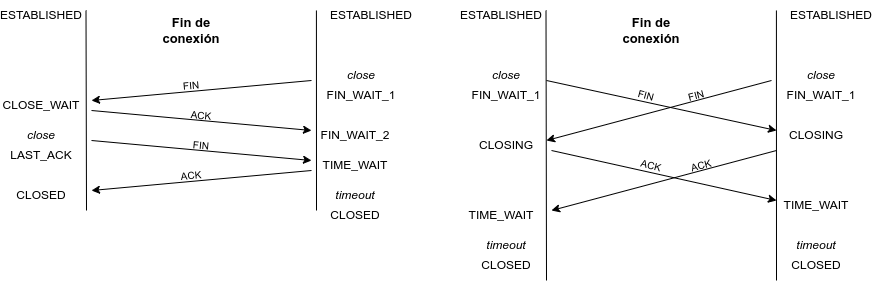
\includegraphics[width=0.8\textwidth
]{images/tcp-closing-conection.png}
	\caption[Diagrama de cierre de conexión]{Diagrama de cierre de conexión}
	\label{fig:tcp-closign-connection}
\end{figure}

Una conexión en el estado \texttt{TIME\_WAIT} no puede pasar al estado \texttt{CLOSED} hasta que haya esperado dos veces la cantidad máxima de tiempo que un datagrama IP podría vivir en Internet. La razón de esto es que, si bien el lado local de la conexión ha enviado un \texttt{ACK} en respuesta al segmento \texttt{FIN} del otro lado, no sabe si el \texttt{ACK} se entregó correctamente. Como consecuencia, el otro lado podría retransmitir su segmento \texttt{FIN}, y este segundo segmento podría retrasarse en la red. 

Si se permitiera pasar directamente al estado CLOSED, entonces otro par de procesos de aplicación podrían llegar y abrir la misma conexión (es decir, usar el mismo par de números de puerto), y el segmento \texttt{FIN} retrasado de la encarnación anterior de la misma inmediatamente iniciaría la terminación de la encarnación posterior.

\subsubsection*{Sliding Window en TCP}
La variante de TCP del algoritmo de ventana deslizante sirve para varios propósitos:
\begin{itemize}
  \item Garantiza la entrega confiable de datos,
  \item Garantiza que los datos se entreguen en orden
  \item Impone un control de flujo entre el remitente y el receptor.
\end{itemize} 

Para lograr lo último, en lugar de tener una ventana deslizante de tamaño fijo, el receptor anuncia un tamaño de ventana al remitente. Esto se hace utilizando el campo \texttt{AdvertisedWindow} en el encabezado TCP. Luego, el remitente está limitado a tener no más \texttt{AdvertisedWindow} bytes de datos no reconocidos en un momento dado. El receptor selecciona un valor adecuado para \texttt{AdvertisedWindow} en función de la cantidad de memoria asignada a la conexión con el fin de almacenar en búfer los datos. De esta manera, se evita que el remitente sobrecargue el búfer del receptor.

\subsubsection*{Envio confiable y ordenado}
El remitente mantiene un búfer de envío que utiliza para almacenar datos que se han enviado pero que aún no se han reconocido, así como datos que ha escrito la aplicación de envío pero que aún no se han transmitido.

En el lado receptor, TCP mantiene un búfer de recepción. Este búfer contiene datos que llegan desordenados, así como datos que están en el orden correcto (es decir, no faltan bytes antes en el flujo) pero que el proceso de aplicación aún no ha tenido la oportunidad de leer.

\begin{figure}[H]
	\centering
	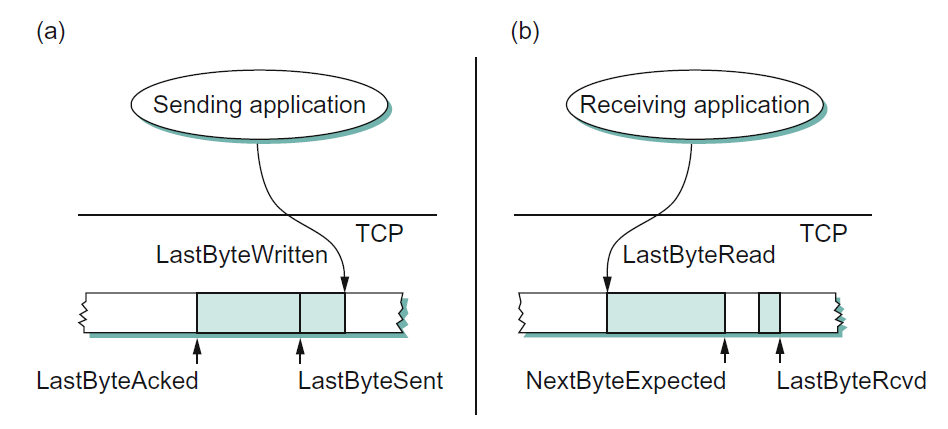
\includegraphics[width=0.8\textwidth
]{images/tcp-buffers.png}
	\caption[Buffers de TCP]{Buffers de TCP}
	\label{fig:tcp-buffers}
\end{figure}

Del lado del remitente, se mantienen tres punteros en el búfer de envío: \texttt{LastByteAcked}, \texttt{LastByteSent} y \texttt{LastByteWritten} y se cumplen las siguientes condiciones:
\begin{itemize}
  \item \(\texttt{LastByteAcked} \leq \texttt{LastByteSent}\): El receptor no puede haber reconocido un byte que aún no se ha enviado
  \item \(\texttt{LastByteSent} \leq \texttt{LastByteWritten}\): TCP no puede enviar un byte que el proceso de aplicación aún no ha escrito.
  \item Ninguno de los bytes a la izquierda de \texttt{LastByteAcked} necesita ser guardado en el búfer porque ya han sido reconocidos, y ninguno de los bytes a la derecha de \texttt{LastByteWritten} necesita ser almacenado en el búfer porque aún no se han generado.
\end{itemize}

Un conjunto similar de punteros (números de secuencia) se mantienen en el lado receptor: \texttt{LastByteRead}, \texttt{NextByteExpected} y \texttt{LastByteRcvd}. Sin embargo, las desigualdades son un poco menos intuitivas, debido al problema de la entrega desordenada:
\begin{itemize}
  \item \(\texttt{LastByteRead} < \texttt{NextByteExpected}\): Un byte no puede ser leído por la aplicación hasta que sea todos los bytes anteriores y ese mismo byte hayan sido recibidos. \texttt{NextByteExpected} apunta al byte inmediatamente después del último byte que cumple con este criterio.
  \item \(\texttt{NextByteExpected} \leq \texttt{LastByteRcvd} + 1\): Si los datos llegaron en orden, \texttt{NextByteExpected} apunta al byte después de \texttt{LastByteRcvd}, mientras que si los datos han llegado desordenados, entonces \texttt{NextByteExpected} apunta al comienzo del primer espacio en los datos.
  \item Los bytes a la izquierda de \texttt{LastByteRead} no necesitan estar en búfer porque ya han sido leídos por el proceso de aplicación local, y los bytes a la derecha de \texttt{LastByteRcvd} no necesitan estar en búfer porque aún no han llegado.
\end{itemize}

\subsubsection*{Control de flujo}
Ambos búferes mencionados en la sección anterior son de algún tamaño finito, denotados como \texttt{MaxSendBuffer} y \texttt{MaxRcvBuffer}.

En TCP, el receptor se debe asegurar qué \[\texttt{LastByteRcvd} - \texttt{LastByteRead} \leq \texttt{MaxRcvBuffer}\]
para evitar la sobrecarga de su búfer. Para esto, controla el tamaño de la ventana deslizante que anuncia al remitente seteando el campo \texttt{AdvertisedWindow} en el encabezado TCP con el valor \[\texttt{MaxRcvBuffer} - ((\texttt{NextByteExpected}-1)-\texttt{LastByteRead})\]
que es la cantidad de espacio libre que tiene en el búfer.

A medida que le llegan los datos, los reconoce siempre que también hayan llegado todos los bytes anteriores. Además, \texttt{LastByteRcvd} se mueve a la derecha (se incrementa), lo que significa que la ventana anunciada potencialmente se reduce. Si se reduce o no depende de qué tan rápido el proceso de la aplicación local está consumiendo datos. Si el proceso local está leyendo datos tan rápido como llegan, entonces la ventanta anunciada se mantiene. Sin embargo, si el proceso receptor se atrasa, tal vez porque realiza una operación muy costosa en cada byte de datos que lee, entonces la ventana anunciada se vuelve más pequeña con cada segmento que llega, hasta que eventualmente llega a 0.

\paragraph{Wraparound:} El número de secuencia utilizado en una conexión determinada podría dar la vuelta, un byte con el número de secuencia \(x\) podría enviarse en un momento determinado, y luego en un momento posterior un segundo byte con el mismo número de secuencia \(x\) podría enviarse. Nuevamente, asumimos que los paquetes no pueden sobrevivir en Internet por más tiempo que el \(MSL\) recomendado. Si esto sucede o no depende de qué tan rápido se pueden transmitir los datos a través de Internet, es decir, qué tan rápido se puede consumir el espacio de número de secuencia de 32 bits.

\paragraph{Manteniendo el pipe lleno:} El valor del \texttt{AdvertisedWindow} debe ser lo suficientemente grande como para permitir que el remitente mantenga el pipe lleno. El receptor es libre de no anunciar una ventana de tamaño máximo (tan grande como lo permite el campo \texttt{AdvertisedWindow}).

El máximo \texttt{AdvertisedWindow} posible se puede calcular como el  producto de la demora y el ancho de banda \(delay\times bandwidth\).

\subsubsection{Transmisión de datos}
TCP usa tres mecanismos para decidir cuando transmitir datos:
\begin{itemize}
  \item TCP mantiene una variable, generalmente llamada \textbf{tamaño máximo de segmento}\\ (\(MSS\)), y envía un segmento tan pronto como ha recopilado \(MSS\) bytes del proceso de envío. 
  Generalmente se establece este valor de tal manera de evitar que la IP local se fragmente.Es decir, \(MSS\) se establece en la unidad máxima de transmisión (MTU) de la red conectada directamente, menos el tamaño de los encabezados TCP e IP.
  \item TCP admite una operación de empuje, y el proceso de envío invoca esta operación para vaciar efectivamente el búfer de bytes no enviados.
  \item El último disparador para transmitir un segmento es que se active un temporizador; el segmento resultante contiene tantos bytes como los que están actualmente almacenados en búfer para su transmisión.
\end{itemize}

\paragraph{Silly Window Syndrome:} Supongamos que el remitente está acumulando bytes para enviar, pero la ventana está actualmente cerrada. Ahora suponga que llega un \texttt{ACK} que abre efectivamente una ventana de pocos bytes. La especificación original no aclaraba que hacer en esta situación y las primeras implementaciones de TCP decidieron transmitir un segmento medio lleno. Después de todo, no hay forma de saber cuánto tiempo pasará antes de que la ventana se abra aún más.

Resulta que esta estrategia de aprovechar agresivamente cualquier ventana disponible conduce a una situación ahora conocida como el \texttt{síndrome de la ventana tonta}.

Si el remitente llena agresivamente un contenedor vacío más pequeño que un \(MSS\) tan pronto como llega, el receptor \(ACK\) ese número de bytes, y por lo tanto el contenedor introducido en el sistema permanece en el sistema indefinidamente. Es decir, se llena e inmediatamente se vacía en cada extremo y nunca se fusiona con contenedores adyacentes para crear contenedores más grandes.

Actualmente, se puede retrasar este sindromehaciendo que el receptor espere a poder aceptar \(MSS\) bytes antes de anunciar una ventana abierta.

Dado que no podemos eliminar la posibilidad de que se introduzca un contenedor pequeño en el flujo, también necesitamos mecanismos para fusionarlos. El receptor puede hacer esto retrasando los ACK: enviando un ACK combinado en lugar de varios más pequeños, pero esta es solo una solución parcial porque el receptor no tiene forma de saber cuánto tiempo es seguro esperar a que llegue otro segmento o para que la aplicación lea más datos.

\paragraph{Algoritmo de Naggle:} Mientras TCP tenga datos en vuelo, el remitente eventualmente recibirá un ACK. Este ACK se puede tratar como un temporizador que se activa, lo que desencadena la transmisión de más datos. El algoritmo de Nagle proporciona una regla simple y unificada para decidir cuándo transmitir:
\begin{itemize}
  \item[] La aplicacion produce \(b\) bytes:
  \begin{itemize}
    \item[] Si \(b \geq  MSS\) y \(\texttt{AdvertisedWindow}\geq MSS\)
     \begin{itemize}
      \item[] Se manda un segmento completo
    \end{itemize}
    \item[] Sino:
    \begin{itemize}
      \item[] Si hay datos que todavia no fueron reconocidos (sin acks)
      \begin{itemize}
        \item[] Acumular datos hasta que el próximo \texttt{ACL} llegue.
      \end{itemize}
      \item[] Sino:
      \begin{itemize}
        \item[] Enviar todos los datos ahora
      \end{itemize}
    \end{itemize}
  \end{itemize}
\end{itemize}

En otras palabras, siempre está bien enviar un segmento completo si la ventana lo permite. También está bien enviar inmediatamente una pequeña cantidad de datos si actualmente no hay segmentos en tránsito, pero si hay algo en vuelo, el remitente debe esperar un ACK antes de transmitir el siguiente segmento.

Debido a que algunas aplicaciones no pueden permitirse tal retraso para cada escritura que realiza en una conexión TCP, la interfaz de socket permite a la aplicación desactivar el algoritmo de Nagel estableciendo la opción TCP \texttt{NODELAY}. Usar esta opción significa que los datos se transmiten lo antes posible.

\subsubsection{Retransmisión adaptativa}
Debido a que TCP garantiza la entrega confiable de datos, retransmite cada segmento si no se recibe un \texttt{ACK} en un cierto período de tiempo. El protocolo establece este tiempo de espera como una función del RTT que espera entre los dos extremos de la conexión. Desafortunadamente, dada la gama de RTT posibles entre cualquier par de hosts en Internet, así como la variación en RTT entre los mismos dos hosts con el tiempo, elegir un valor de tiempo de espera apropiado no es tan fácil. Para abordar este problema, TCP utiliza un mecanismo de retransmisión adaptativo.

\paragraph{Algortimo original:} Cada vez que TCP envía un segmento de datos, registra el tiempo. Cuando llega un ACK para ese segmento, TCP lee el tiempo nuevamente y luego toma la diferencia entre estos dos tiempos como un \texttt{SampleRTT}. TCP luego calcula un \texttt{EstimatedRTT} como un promedio ponderado entre la estimación anterior y esta nueva muestra. Es decir,
  \[ \texttt{EstimatedRTT} = \alpha\times \texttt{EstimatedRTT} + (1-\alpha)\times \texttt{SampleRTT} \]

El parámetro \(\alpha\) se selecciona para suavizar el \texttt{EstimatedRTT}. Un \(\alpha\) pequeño realiza un seguimiento de los cambios en el RTT, pero tal vez esté demasiado influenciado por fluctuaciones temporales. Por otro lado, un \(\alpha\) grande es más estable pero quizás no sea lo suficientemente rápido como para adaptarse a cambios reales. La especificación original de TCP recomendó una configuración de \(\alpha\) entre \(0.8\) y \(0.9\).

TCP luego usa \texttt{EstimatedRTT} para calcular el tiempo de espera de una manera bastante conservadora:
\[ \texttt{TimeOut} = 2\times \texttt{EstimatedRTT}\]

\paragraph{Algoritmo de Karn/Partridge:} Un ACK no reconoce realmente una transmisión; en realidad, reconoce la recepción de datos. En otras palabras, cada vez que se retransmite un segmento y luego llega un ACK al remitente, es imposible determinar si este ACK debe asociarse con la primera o la segunda transmisión del segmento con el fin de medir el tiempo de ida y vuelta de la muestra. Es necesario saber qué transmisión asociar con el fin de calcular un \texttt{SampleRTT} preciso.  

Este algoritmo, resuelve esto haciendo que solo se calcule un \texttt{SampleRTT} para segmentos que fueron transmitidos una sola vez. Cada vez que TCP retransmite un segmento, duplica el valor del siguiente timeout (usa \textbf{exponential backoff}). Esta última decisión se debe a que la congestión es la causa más probable de segmentos perdidos, lo que significa que el remitente de un mensaje no debe reaccionar agresivamente a un timeout. De hecho, cuanto más veces se agota el tiempo de espera de la conexión, más cautelosa debe ser la fuente.

\paragraph{Algoritmo de Jacobson/Karels:} Es una mejora al algoritmo anterior. Si la variación entre las muestras es pequeña, entonces el \texttt{EstimatedRTT} puede ser considerado confiable y no hay razón para multiplicar esta estimación por 2 para calcular el timeout. Por otro lado, una gran varianza en las muestras sugiere que el valor de timeout no debe estar demasiado acoplado al \texttt{EstimatedRTT}. Para tener en cuenta estas situaciones, una vez obtenido un \texttt{SampleRTT}, se calcula el \texttt{TimeOut} de la siguiente manera:
\[\texttt{Difference} = \texttt{SampleRTT} - \texttt{EstimatedRTT}\]
\[ \texttt{EstimatedRTT} = \texttt{EstimatedRTT} + (\delta\times\texttt{Difference})\]
\[Deviation = Deviation + (\delta\times(|\texttt{Difference}| - \texttt{Deviation}))\]
\[\texttt{TimeOut} = \mu\times\texttt{EstimatedRTT} + \phi\times\texttt{Deviation}\]

Donde \(\delta\) es una valor valor entre 0 y 1. \(\mu = 1\) y \(\phi=4\).  De esta manera, si la varianza es pequeña, el \texttt{Timeout} es cercano al \texttt{EstimatedRTT}, y si la varianza es grande, entonces \texttt{Deviation} domina el calculo.

\newpage

% Traducir del ingles
account. Intuitively, if the varia
tion
among samples is small, then the EstimatedRTT can be better trusted
and there is no reason for multiplying this estimate by 2 to compute the
timeout. On the other hand, a large variance in the samples suggests that
the timeout value should not be too tightly coupled to the EstimatedRT
% Al español:
Intuitivamente, si la variación entre las muestras es pequeña, entonces el \texttt{EstimatedRTT} puede ser mejor confiable y no hay razón para multiplicar esta estimación por 2 para calcular el tiempo de espera. Por otro lado, una gran varianza en las muestras sugiere que el valor de tiempo de espera no debe estar demasiado acoplado al \texttt{EstimatedRTT}.



\newpage
\red{\section*{Congestión}
Introducción al problema de congestión. Curvas de Trafico Enviado vs entregado. Resultado con buffer infinito. Causas de congestión. Control de flujo vs Control de congestión. Taxonomia de Yang y Redan. Soluciones de lazo cerrado y abierto. Concepto de sistemas realimentados. Métricas a sensar para las realimentación. Realimentación implícita y explicita. Determinación de la performance.}


\newpage
\red{\section*{Congestión}
Introducción al problema de congestión. Curvas de Trafico Enviado vs entregado. Resultado con buffer infinito. Causas de congestión. Control de flujo vs Control de congestión. Taxonomia de Yang y Redan. Soluciones de lazo cerrado y abierto. Concepto de sistemas realimentados. Métricas a sensar para las realimentación. Realimentación implícita y explicita. Determinación de la performance.}

\newpage
\section{Seguridad}
Un protocolo provee \textbf{cofidencialidad} si encripta los mensajes para prevenir que un atacante pueda leerlos. Si además oculta la cantidad de información o el destino del mensaje, entonces ofrece \textbf{Confidencialidad de tráfico}.

Un atacante que no puede leer el contenido del mensaje encriptado sigue siendo capaz de modificar los paquetes nterceptados a través de una red y generar contenido válido. Si el protocolo implementa técnicas para detectar si un paquete fue modificado en el camino, entonces se dice que ofrece \textbf{Integridad}.

Otra amenaza para el cliente es ser dirigido sin saberlo a un sitio web falso. Esto puede resultar de un \textbf{DNS Attack}, en el que se ingresa información falsa en un servidor DNS o en la caché del DNS de la computadora del cliente. Esto lleva a traducir una URL correcta en una dirección IP incorrecta. Un protocolo que garantiza que realmente está hablando con quien cree que está hablando se dice que proporciona \textbf{autenticación}. La autenticación implica integridad, ya que no tiene sentido decir que un mensaje proviene de un cierto participante si ya no es el mismo mensaje.

Si el atacante en vez de crear un sitio falso, logra modificar los archivos de uno existente, Ese es un problema de \textbf{control de acceso}: hacer cumplir las reglas sobre quién está autorizado a hacer qué. Los sitios web también han sido objeto de ataques de denegación de servicio (DoS), durante los cuales los clientes potenciales no pueden acceder al sitio web porque está siendo abrumado por solicitudes falsas.  Afecta el nivel de \textbf{disponibilidad}.

\subsection{Principios de cifrado}
El cifrado transforma un mensaje de tal manera que se vuelve ininteligible para cualquier parte que no tenga el secreto de cómo revertir la transformación. El remitente aplica una función de cifrado al mensaje de texto plano original y envía el resultado a través de la red. El receptor aplica una función de descifrado al mensaje que le llega para recuperar el mensaje original.

La transformación representada por una función de encriptado y su función de descifrado correspondiente se llama \textbf{cipher}.

Las funciones de cifrado y descifrado son de conocimiento público pero están parametrizadas por una clave secreta. Una razón para este principio es que si se depende de que el cifrado se mantenga en secreto, entonces hay que retirar el cifrado (no solo las claves) cuando sea vulnerado. Esto significa cambios potencialmente frecuentes de cifrado, lo cual es problemático, ya que toma mucho trabajo desarrollar uno nuevo. Además, una de las mejores formas de saber que un cifrado es seguro es usarlo durante mucho tiempo, si nadie lo rompe, probablemente lo sea.

Los mejores algoritmos de cifrado pueden evitar que el atacante deduzca la clave incluso cuando este conoce tanto el texto plano como el texto cifrado. Esto deja al atacante sin otra opción que probar todas las claves posibles usando fuerza bruta. La fuerza bruta puede ser computacionalmente ineficiente si se eligue un espacio de claves lo suficientemente grande y si las operaciones de cifrado y descifrado son lo suficientemente costosas. Una de las idifcultades de esta elección es que las velocidad de computo aumentan con el tiempo, por lo que lo que ahora puede ser computacionalmente imposible, en el futuro quizas sea posible.

\subsubsection{Cifrado en bloques}
La mayoría de los cifrados son \textbf{cifrados de bloque}: se definen para tomar como entrada un bloque de texto plano de un cierto tamaño fijo, típicamente de 64 a 128 bits. El uso de un cifrado de bloque para encriiptar cada bloque de forma independiente, conocido como \textbf{cifrado de libro electrónico (Electronic Cipher Book - ECB)}, tiene la debilidad de que un valor de bloque de texto plano dado siempre dará como resultado el mismo bloque de texto cifrado. Por lo tanto, los valores de bloque recurrentes en el texto plano son reconocibles como tales en el texto encriptado, lo que hace que sea mucho más fácil para un criptoanalista romper el cifrado.

Para evitar esto, los cifrados de bloque siempre se amplían para hacer que el texto resultate para un bloque varíe según el contexto. Las formas en que se puede ampliar un cifrado de bloque se llaman \textbf{modos de operación}. Un modo de operación común es el \textbf{Cipher Block Chaining (CBC)}, en el que cada bloque de texto plano se XORea con el texto cifrado del bloque anterior antes de ser encriptado. El resultado es que el texto cifrado de cada bloque depende en parte de los bloques anteriores. Dado que el primer bloque no tiene precedente, se lo xorea con un número random llamado \textbf{vector de inicialización} que se acuerda al principio de la comunicación para que el receptor pueda descifrarlo.

\subsubsection{Cifrados de clave secretas}
En un cifrado de clave secretas o clave simetrica, ambos participantes de la comunicación comparten la misma clave. Osea que el mensaje es encriptado usando una clave particular y luego es desencriptado usando la misma clave. El problema es que la clave debe ser compartida entre los participantes de la comunicación, lo que puede ser difícil de lograr. Además, si la clave se ve comprometida, entonces todos los mensajes encriptados con esa clave también se ven comprometidos.

El Instituto Nacional de Estándares y Tecnología (NIST) de los EE. UU. ha emitido estándares para una serie de cifrados de clave secreta. El \textbf{Estándar de cifrado de datos (Data Encryption Standard - DES)} fue el primero, y ha resistido la prueba del tiempo en el sentido de que no se ha descubierto ningún ataque criptanalítico mejor que la búsqueda de fuerza bruta. Sin embargo, las claves de DES son relativamente cortas (56 bits), lo que significa que un atacante con suficiente poder de cómputo puede probar todas las claves posibles en un tiempo razonable. Por lo tanto, DES ya no se considera seguro.

Se actualizó este estandar con el cifrado \textbf{3DES} que aplica tres claves DES (168 bits) para encriptar el mensaje de la siguiente manera:
\begin{enumerate}
  \item Usa la primer clave para encriptar el mensaje original.
  \item La segunda se usa para desencriptar el resultado del paso anterior. Osea se aplica la función de descifrado de DES para obtener un nuevo mensaje.
  \item La tercer clave se usa para encriptar el resultado del paso anterior. Osea se aplica la función de cifrado de DES para obtener el mensaje final.
\end{enumerate}

El desencriptado implica hacer la inversa de cada uno de esos pasos: Desencriptar con la tercer clave, encriptar con la segunda y desencriptar con la primera.

Actualmente, 3DES está siendo reemplazado por el estándar \textbf{Advanced Encryption Standard (AES)} emitido por NIST que soporta claves de 128, 192 y 256 bits.

\subsection{Cifrados de clave pública}
Una alternativa a los cifrados de clave secreta son los cifrados de clave pública. En lugar de una sola clave compartida por dos participantes, un cifrado de clave pública utiliza un par de claves relacionadas, una para el cifrado y otra diferente para el descifrado. El par de claves es "propiedad" de un solo participante. El propietario mantiene la clave de descifrado en secreto para que solo él pueda descifrar los mensajes; esa clave se llama \textbf{clave privada}. Además, hace pública la clave de cifrado para que cualquiera pueda cifrar mensajes que le estén destinados; esa clave se llama \textbf{clave pública}.

Para que un esquema de este tipo funcione, no debe ser posible deducir la clave privada a partir de la pública.

\begin{figure}[H]
	\centering
	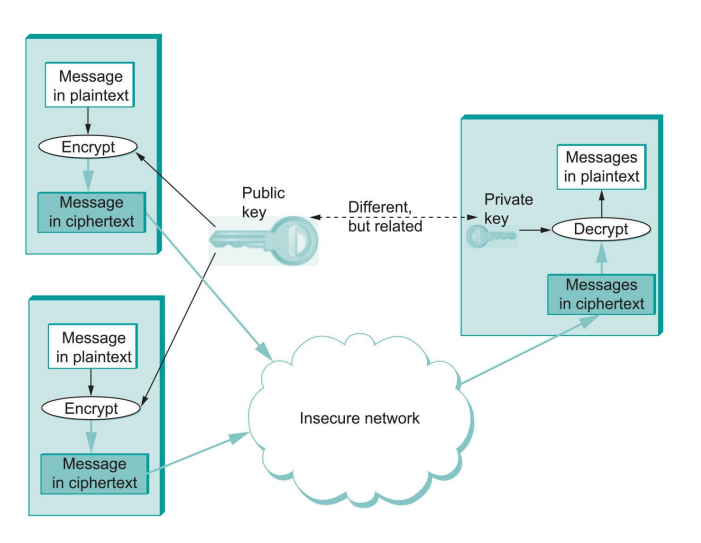
\includegraphics[width=0.5\textwidth
]{images/public-key-encryption.png}
	\caption[Encriptación con clave pública]{Encriptación con clave pública}
	\label{fig:public-key-encryption}
\end{figure}

Una clave para un cifrado de clave secreta proporciona un canal bidireccional entre dos participantes: cada participante tiene la misma clave (simétrica) que cualquiera puede usar para encriptar o desencriptar mensajes en cualquier dirección. Un par de claves pública / privada, en contraste, proporciona un canal unidireccional y de muchos a uno: desde todos los que tienen la clave pública hasta el único propietario de la clave privada.

Una propiedad adicional importante de los cifrados de clave pública es que la clave privada de "descifrado" se puede usar con el algoritmo de cifrado para cifrar mensajes de modo que solo se puedan descifrar usando la clave pública de "cifrado". Esta propiedad, si bien no nos ofrece confidencialidad, ya que cualquiera podría descifrar el mensaje, nos permite autenticar el mensaje. Si el mensaje se descifra correctamente, entonces el receptor pued estar seguro que el mensaje fue enviado por la persona que lo encriptó. Esto se llama \textbf{firma digital}.

El algoritmo de clave pública más conocido es el RSA (Rivest, Shamir, Adleman). Este algoritmo aprovecha el alto costo computacional de factorizar números grandes. El problema de encontrar una manera eficiente de factorizar números es uno en el que los matemáticos han trabajado sin éxito desde mucho antes de que apareciera RSA en 1978, y la resistencia posterior de RSA a la criptoanálisis ha fortalecido aún más la confianza en su seguridad. Desafortunadamente, RSA necesita claves relativamente grandes, al menos 1024 bits, para ser seguro. Las claves RSA son mas grandes que las claves para los cifrados de clave secreta porque es más rápido romper una clave privada RSA factorizando el número grande en el que se basa el par de claves que buscando exhaustivamente el espacio de claves.

En general, los cifrados de clave pública son usados principalmente para autenticar y distribuir claves secretas (simétricas) para su uso durante la comunicación entre dos entidades. Esto se debe a que los cifrados de clave pública son computacionalmente costosos en comparación con los cifrados de clave secreta.


\subsubsection{Autenticadores}
Un autenticador es un valor, que se incluye en un mensaje transmitido, que puede ser usado para verificar simultaneamente la autenticidad y la integridad de los datos de un mensaje.

Las sumas de verificación (checksums) y las comprobaciones de redundancia cíclica (CRC) son piezas de información agregadas a un mensaje para que el receptor detecte cuando el mensaje ha sido modificado inadvertidamente por errores de bits. Un concepto similar se aplica a los autenticadores, con el desafío adicional de que la corrupción del mensaje probablemente sea realizada deliberadamente por alguien que quiera que la corrupción pase desapercibida.

Para admitir la autenticación, un autenticador incluye alguna prueba de que quien creó el autenticador conoce un secreto que solo conoce el supuesto remitente del mensaje. 

\paragraph{Cryptographic checksum: }  Combina encriptación y una función hash criptográfica. Los algoritmos hash criptográficos se tratan como conocimiento público, como con los algoritmos de cifrado. Una función hash criptográfica (también conocida como suma de verificación criptográfica) es una función que produce suficiente información redundante sobre un mensaje para exponer cualquier manipulación. El resultado de esta función se llama \textbf{Message Digest} y se agrega al final del mensaje antes de encriptar. El receptor puede verificar la integridad del mensaje descifrando el mensaje y luego aplicando la función hash criptográfica al mensaje descifrado. Si el resultado coincide con el Message Digest recibido, entonces el mensaje no se ha modificado. 

Todos los message digests generados por la función son del mismo tamaño, idependientemente de la longitud del mensaje original. Dado que el espacio de mensajes posibles es más grande que el espacio de message digests, habrá mensajes distintos que tienen el mismo valor de message digest. Para que la función de hash sea segura en necesario que tenga la propiedad \textbf{one-way}: Debe ser computacionalmente imposible encontrar un mensaje que produzca el mismo message digest que el mensaje original. 

Una condición necesaria para que esto se cumpla es que el output de esta función debe estar distribuido uniformemente en el espacio de message digests. Si no lo está, entonces habrá regiones del espacio de message digests que son más probables que otras y, por lo tanto, más fáciles de encontrar.

Ha habido varios algoritmos hash criptográficos comunes a lo largo de los años, incluidos Message Digest 5 (MD5) y la familia Secure Hash Algorithm (SHA). Las debilidades de MD5 y las versiones anteriores de SHA han sido conocidas por algún tiempo, lo que llevó al NIST a recomendar el uso de SHA-3 en 2015.

\subsubsection{Firma Digital} Un digest encriptado con un algoritmo de clave pública pero usando la clave privada se llama firma digital porque proporciona no repudio como una firma escrita. El receptor de un mensaje con una firma digital puede demostrar a cualquier tercero que el remitente realmente envió ese mensaje, porque el tercero puede usar la clave pública del remitente para verificarlo por sí mismo.

\subsubsection{Message Authentication Code (MAC)} 
Se usa una clave secreta (conocida solo por el remitente y el receptor) para crear un código MAC que se concatena al mensaje de texto plano (antes de encriptar). Cuando el recptor recibe  el mensaje, calcul su propio MAC usando el texto del mensaje que le llegó y la clave secreta. Si el código MAC calculado coincide con el código MAC recibido, entonces el receptor puede estar seguro de que el mensaje no se ha modificado y que fue enviado por alguien que conoce la clave secreta. 

Una variación de este esquema es el \textbf{HMAC} en la que el mensaje se concatena la clave secreta y se pasa a una función de hash criptográfica. El resultado que devuelve está función es el codigo que se concatena al mensaje antes de ser enviado.

\subsection{Distribución de claves}
Para poder usar autenticadores o cifrado de clave secreta, los participantes deben saber qué claves usar.

\paragraph{Session Key:} Una clave secreta que se genera para su uso en una sola sesión de comunicación, es válida durante un pequeño intervalo de tiempo. Cada sesión tiene un clave diferente y esta es determinada por medio de algún protocolo de protocolo especial. 

\paragraph{Predistributed Keys:} Son claves que se distribuyen antes de que se necesiten. En general, son manejadas por un centro de administración de claves que permite a los usuarios establecer sesiones de comunicación segura entre ellos. En general, este tipo de claves solo se utiliza al comienzo de una comunicación para establecer una clave de sesión entre los participantes para luego pasar a usar esa clave de sesión para el resto de la comunicación.

Hay dos razones para que estas claves se usen de esta forma:
\begin{itemize}
  \item Limitar la cantidad de veces que se usa una clave resulta en menos tiempos para ataques que sean intensivos computacionalmente, menos texto cifrado que un atacante pueda interceptar y menos información expuesta si la clave se ve comprometida.
  \item Las claves públicas son superiores a las claves secretas en términos de autenticación y establecimiento de clave, pero es demasiado lento cifrar mensajes completos con ellas.
\end{itemize}

\subsubsection{Predistribución de claves públicas}
Los algoritmos para crear un par de claves publica/privadas son de público conocimiento y es facil de econtrar software que lo haga. 

Supongamos que Alice quiere usar cifrado asimétrico, entonces podría generar su propio par de claves y publicar la clave publica. El problema es como publicar la clave de tal maner que otros usuarios puedan estar seguros de que la clave publica realmente le pertenece a ella.

\subsubsection*{Public Key Infrastructure (PKI)}
Una PKI comienza con la capacidad de verificar identidades y vincularlas a claves fuera de banda. Por "fuera de banda", nos referimos a algo fuera de la red y de las computadoras que la componen, por ejemplo, si Alice y Bob son individuos que se conocen, entonces podrían reunirse en la misma habitación y Alice podría darle su clave pública a Bob directamente, tal vez en una tarjeta de presentación.

Establecer claves fuera de banda no parece que escalaría bien, pero es suficiente para arrancar una PKI. El conocimiento de Bob de que la clave de Alice es \(X\) puede ser ampliamente, difundido de forma escalable usando una combinación de firmas digitales y un concepto de confianza.

Una declaración firmada digitalmente de una vinculación de clave pública se llama \textbf{certificado de clave pública}, o simplemente certificado. Este certificado debe contener:
\begin{itemize}
  \item La identidad de la entidad que está siendo certificada.
  \item La clave pública de esa entidad.
  \item La identidad del que firma el certificado
  \item La firma digital
  \item Un identificador del algoritmo de firma digital que se usó para crear la firma.
\end{itemize}

\subsubsection*{Autoridades de certificación}
Si \(X\) certifica que una cierta clave pública pertenece a \(Y\), y luego \(Y\) certifica que otra clave pública pertenece a \(Z\), entonces existe una cadena de certificados de \(X\) a \(Z\), incluso si \(X\) y \(Z\) nunca se han conocido.

Una \textbf{autoridad de certificación} o \textbf{autoridad de certificados (CA)} es una entidad que se afirma que es confiable para verificar identidades y emitir certificados de clave pública.

Hay CA comerciales, CA gubernamentales e incluso CA gratuitas. Para usar una CA, se debe conocer su clave, la cual se puede aprender la clave de una CA si puede obtener una cadena de certificados que comienza con una CA cuya clave ya conoce. Luego puede creer cualquier certificado firmado por esa nueva CA. 

Una forma común de construir tales cadenas es organizarlas en una jerarquía estructurada en árbol. En la parte superior de la jerarquía se encuentra una CA raíz, que es una CA que se considera confiable sin necesidad de un certificado. La CA raíz emite certificados para otras CA, que a su vez emiten certificados para otras CA, y así sucesivamente. 

Hay algunos problemas importantes con la construcción de cadenas de confianza. Lo más importante es que, incluso si se está seguro de que se tiene la clave pública de la CA raíz, debemos asegurar que cada CA, desde la raíz hacia abajo, esté haciendo su trabajo correctamente. Si solo una CA en la cadena está dispuesta a emitir certificados a entidades sin verificar sus identidades, entonces lo que parece ser una cadena válida de certificados se vuelve insignificante.

Firefox e Internet Explorer vienen pre-equipados con certificados para un conjunto de CA; en efecto, el productor del navegador ha decidido que estas CA y sus claves pueden ser confiables. Un usuario también puede agregar CA a las que su navegador reconoce como confiables. Estos certificados son aceptados por Secure Socket Layer (SSL) / Transport Layer Security (TLS), el protocolo más utilizado para asegurar las transacciones web.

\subsubsection*{Web of trust}
Un modelo alternativo de confianza es la red \textbf{Pretty Good Privacy (PGP)}:  es un sistema de seguridad para correo electrónico, en el cual las direcciones de email son las identidades a las que se vinculan las claves y por las que se firman los certificados. En consonancia con las raíces de PGP como protección contra la intrusión del gobierno, no hay CA. En cambio, cada individuo decide en quién confía y cuánto confía en ellos; en este modelo, la confianza es una cuestión de grado. Un certificado puede incluir un nivel de confianza que indique cuán confiado está el firmante de la vinculación de claves reclamada en el certificado, por lo que un usuario determinado podrá decidir esperar varios certificados que atestigüen la misma vinculación de claves antes de estar dispuesto a confiar en ella.

En resumen, PGP reconoce que el problema de establecer la confianza es un asunto bastante personal y les da a los usuarios la materia prima para tomar sus propias decisiones en lugar de asumir que todos están dispuestos a confiar en una sola estructura jerárquica de CA.

\subsubsection*{Revocación de certificados}
En el caso de que un certificado haya sido vulnerado, las CA agrega este certificado a una \textbf{Lista de certificados revocados (Certificate Revocation List - CRL)} que firma digitalmente. Los usuarios pueden descargar la CRL y verificar si un certificado dado está en ella. Si lo está, entonces el certificado se ha revocado y no debe confiarse. Además, cada certificado tiene un tiempo de vida, después del cual se considera inválido y son eliminados de esta lista.

\subsubsection{Predistribución de claves secretas}
Existen entidades conocidas como \textbf{Key Distribution Centers (KDC)} que se encargan de distribuir claves secretas. Un KDC es un servidor que comparte una clave secreta con cada participante de la comunicación. Cuando Alice quiere comunicarse con Bob, se comunica con el KDC usando claves asimétricas indicandole sus intenciones. El KCD genera una clave secreta que le envia a Alice y a Bob. Luego Alice y Bob pueden comunicarse usando esa clave secreta.

\subsection{Protocolos
 de autenticación}
\paragraph{Reply Attack:} Un ataquente retransmite una copia de un mensaje que ya se envió. A pesar de que no es la primera encarnación del mensaje, el autenticador es válido y como no fue modificado puede ser correctamente descifrado. Sin embargo, el mensaje puede no ser válido en el contexto actual. Por ejemplo, si el mensaje es una solicitud de transferencia de fondos, entonces el atacante podría retransmitir la solicitud para que se ejecute dos veces. Necesitamos una solución que provea \textbf{Originalidad}.

Una veración de este ataque es el \textbf{supress-replay attack} en el que el atacante intercepta un mensaje y lo demora para que sea recibido en algún momento que no sea el apropiado. En este caso, aunque el mensaje es original, no es oportuno. Necesitamos una solución que provea \textbf{Timeliness}.

\subsubsection{Técnicas de Orginialidad y Timeliness}
Un enfoque es incluir una marca de tiempo en el mensaje. La marca de tiempo en sí debe ser a prueba de manipulaciones, por lo que debe estar cubierta por el autenticador. La principal desventaja de las marcas de tiempo es que requieren sincronización de relojes distribuidos. Dado que nuestro sistema dependería de la sincronización, la sincronización de relojes en sí misma debería defenderse contra las amenazas de seguridad, además de los desafíos habituales de la sincronización de relojes.

Otro enfoque es incluir, en el mensaje, un \textbf{nonce}, un número aleatorio que se usa solo una vez. Los participantes pueden detectar ataques de repetición verificando si un nonce se ha usado previamente. Desafortunadamente, esto requiere que se mantenga un log de los nonces ya usados, lo que puede ser difícil de escalar.

\begin{figure}[H]
	\centering
	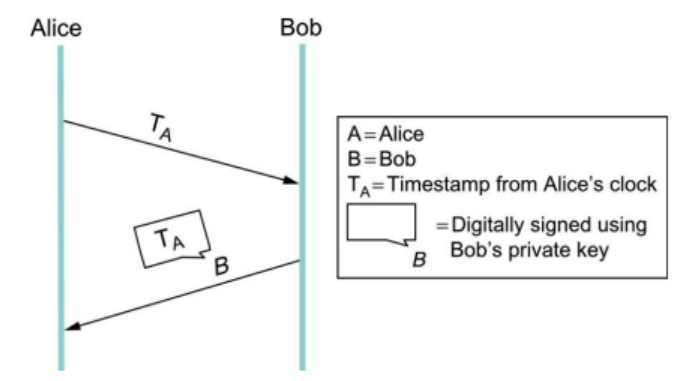
\includegraphics[width=0.5\textwidth
]{images/response-challenge-protocol.png}
	\caption[Protocolo response-challenge]{Protocolo response-challenge basado en timestamps}
	\label{fig:response-challenge-protocol}
\end{figure}

\subsubsection*{Protocolos de autenticación de clave asimétrica}
\begin{figure}[H]
	\centering
	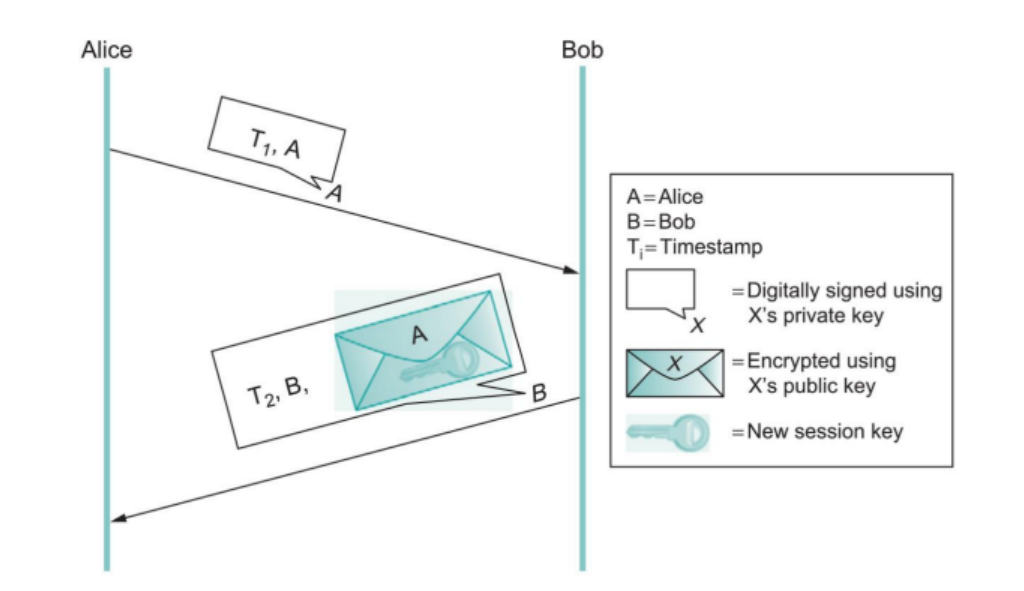
\includegraphics[width=0.5\textwidth
]{images/public-key-authentication.png}
	\caption[Protocolo de autenticación con clave asimétricas]{Protocolo de autenticación con clave asimétricas con sincronización de clocks}
	\label{fig:public-key-authentication}
\end{figure}

Alice envía a Bob un mensaje con un timestamp y su identidad en texto plano más su firma digital. Bob usa la firma digital para autenticar el mensaje y el timestamp para verificar su frescura. Bob envía un mensaje de vuelta con una timestamp y su identidad en texto plano, así como una nueva clave de sesión encriptada (para confidencialidad) usando la clave pública de Alice, todo firmado digitalmente. Alice puede verificar la autenticidad y la frescura del mensaje, por lo que sabe que puede confiar en la nueva clave de sesión. Para lidiar con la sincronización imperfecta del reloj, las marcas de tiempo podrían aumentarse con nonces.

\begin{figure}[H]
	\centering
	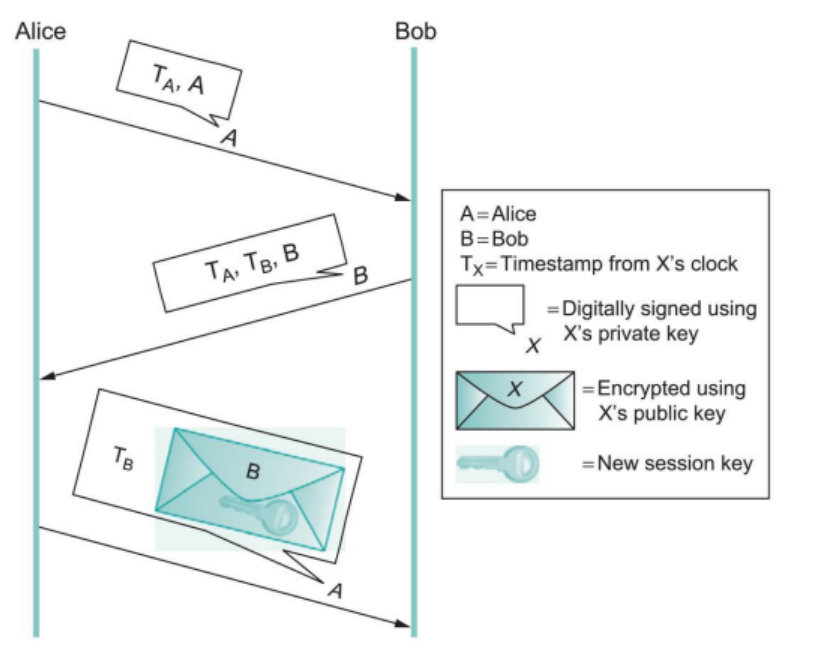
\includegraphics[width=0.5\textwidth
]{images/public-key-authentication-2.png}
	\caption[Protocolo de autenticación con clave asimétricas]{Protocolo de autenticación con clave asimétricas sin sincronización de clocks}
	\label{fig:public-key-authentication-2}
\end{figure}
En este protocolo, Alice nuevamente envía a Bob un mensaje firmado digitalmente con una marca de tiempo y su identidad. Debido a que sus relojes no están sincronizados, Bob no puede estar seguro de que el mensaje sea nuevo. Bob envía un mensaje firmado digitalmente con la marca de tiempo original de Alice, su propia marca de tiempo y su identidad. Alice puede verificar la frescura de la respuesta de Bob comparando su tiempo actual con la marca de tiempo que se originó con ella. Luego le envía a Bob un mensaje firmado digitalmente con su marca de tiempo original y una nueva clave de sesión encriptada usando la clave pública de Bob. Bob puede verificar la frescura del mensaje porque la marca de tiempo provino de su reloj, por lo que sabe que puede confiar en la nueva clave de sesión. Las marcas de tiempo esencialmente sirven como nonces convenientes, e incluso este protocolo podría usar nonces en su lugar.

\subsubsection*{Protocolos de autenticación de clave simétrica}
\begin{figure}[H]
	\centering
	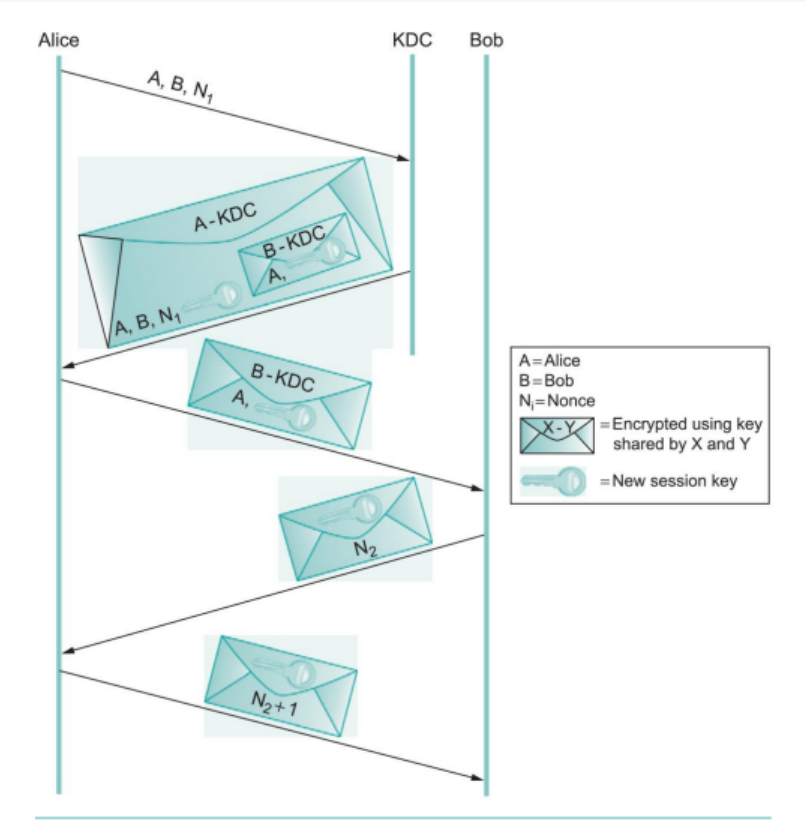
\includegraphics[width=0.5\textwidth]{images/kcd-autenthication.png}
	\caption[Protocolo de autenticación con KDC]{Protocolo de autenticación con KDC}
	\label{fig:kcd-authentication}
\end{figure}
El nonce en los primeros dos mensajes es para asegurarle a Alice que la respuesta del KDC es fresca. Los segundos y terceros mensajes incluyen la nueva clave de sesión y la identificación de Alice, encriptados juntos usando la clave maestra de Bob. Es una especie de versión de clave secreta de un certificado de clave pública; es, en efecto, una declaración firmada por el KDC (porque el KDC es la única entidad además de Bob que conoce la clave maestra de Bob) que la clave de sesión adjunta es propiedad de Alice y Bob.

Notar que el KDC no autentica realmente el mensaje inicial de Alice y no se comunica con Bob en absoluto. En cambio, utiliza su conocimiento de las claves públicas de Alice y Bob para construir una respuesta que sería inútil para cualquier persona que no sea Alice (porque solo Alice puede descifrarla) y que contiene los ingredientes necesarios para que Alice y Bob realicen el resto del protocolo de autenticación ellos mismos.

\newpage
%Traducir:
Note that the KDC does not actually authenticate Alice’s initial 
message and does not communicate with Bob at all. Instead, the KDC 
uses its knowledge of Alice’s and Bob’s master keys to construct a reply 
that would be useless to anyone other than Alice (because only Alice can 
decrypt it) and contains the necessary ingredients for Alice and Bob to 
perform the rest of the authentication protocol themselves.
% Al español:
Tenga en cuenta que el KDC no autentica realmente el mensaje inicial de Alice y no se comunica con Bob en absoluto. En cambio, el KDC utiliza su conocimiento de las claves maestras de Alice y Bob para construir una respuesta que sería inútil para cualquier persona que no sea Alice (porque solo Alice puede descifrarla) y contiene los ingredientes necesarios para que Alice y Bob realicen el resto del protocolo de autenticación ellos mismos.

\red{

\section{Seguridad}
Seguridad en Redes. Marco de Trabajo. Criptografía. Seguridad. Privacidad. Protocolos de Clave Pública y Privada. Algoritmos: DES, 3DES, AES, RSA, MD5 y SHA .Ventajas y desventajas de cada uno. Sus aplicaciones (Autorización, Firma, Confidencialidad e Integridad). Distribución de Claves Públicas. Firewalls. Tunneling. Conceptos de amenazas, ataques, intrusiones.
}

\end{document}

